
\documentclass[aspectratio=169,14pt]{beamer}

% =========================================================
% PAGE SIZE
% =========================================================

\geometry{
    paperwidth=16in,
    paperheight=8.5in
}

% =========================================================
% PACKAGES
% =========================================================

\usepackage{graphicx}
\usepackage{booktabs}
\usepackage{array}
\usepackage{fontawesome5}
\usepackage[table]{xcolor}
\usepackage{tikz}
\usetikzlibrary{positioning,calc}
\usepackage{ragged2e}
\usepackage{amssymb}

% =========================================================
% THEME
% =========================================================

\usetheme{default}

\setbeamertemplate{navigation symbols}{}
\setbeamertemplate{itemize items}[circle]

% =========================================================
% COLORS
% =========================================================

\definecolor{Primary}{HTML}{1565C0}
\definecolor{PrimaryDark}{HTML}{0D47A1}
\definecolor{Secondary}{HTML}{E3F2FD}

\definecolor{Success}{HTML}{2E7D32}
\definecolor{SuccessLight}{HTML}{E8F5E9}

\definecolor{Warning}{HTML}{F9A825}
\definecolor{WarningLight}{HTML}{FFF8E1}

\definecolor{Danger}{HTML}{C62828}
\definecolor{DangerLight}{HTML}{FFEBEE}

\definecolor{Dark}{HTML}{263238}
\definecolor{MediumGray}{HTML}{607D8B}
\definecolor{LightGray}{HTML}{ECEFF1}
\definecolor{StepGray}{HTML}{78909C}

% =========================================================
% GLOBAL TYPOGRAPHY
% =========================================================

\setbeamercolor{normal text}{
    fg=Dark,
    bg=white
}

\setbeamercolor{frametitle}{
    fg=PrimaryDark
}

\setbeamercolor{structure}{
    fg=Primary
}

\setbeamercolor{alerted text}{
    fg=Danger
}

\setlength{\parindent}{0pt}

% =========================================================
% GLOBAL SPACING
% =========================================================

\newlength{\TutorialGap}
\setlength{\TutorialGap}{0.12cm}

\newlength{\SectionGap}
\setlength{\SectionGap}{0.25cm}

% =========================================================
% FRAME TITLE
% =========================================================

\setbeamertemplate{frametitle}{
    \vspace{0.22cm}

    \noindent
    {\color{PrimaryDark}
    \fontsize{25}{30}\selectfont
    \bfseries
    \insertframetitle}

    \vspace{0.10cm}

    {\color{Primary}
    \rule{\textwidth}{1.1pt}}

    \vspace{0.08cm}
}

% =========================================================
% FOOTER
% =========================================================

\setbeamertemplate{footline}{
    \leavevmode
    \hbox{

        \begin{beamercolorbox}[
            wd=.82\paperwidth,
            ht=0.50cm,
            dp=0.15cm,
            leftskip=.42cm
        ]{author in head/foot}

            \fontsize{10}{12}\selectfont
            \textbf{TJI INVENTORY NON DAGANG}

        \end{beamercolorbox}

        \begin{beamercolorbox}[
            wd=.18\paperwidth,
            ht=0.50cm,
            dp=0.15cm,
            center
        ]{date in head/foot}

            \fontsize{10}{12}\selectfont
            \insertframenumber/\inserttotalframenumber

        \end{beamercolorbox}

    }
}

% =========================================================
% SECTION LABEL
% =========================================================

\newcommand{\sectionlabel}[1]{
    {\fontsize{20}{24}\selectfont
    \textbf{\color{Primary}#1}}
}

% =========================================================
% INFO BOX
% =========================================================

\newcommand{\infobox}[2]{
    \begin{tikzpicture}
        \node[
            draw=Primary,
            line width=1pt,
            fill=Secondary,
            rounded corners=6pt,
            inner xsep=12pt,
            inner ysep=9pt,
            text width=\dimexpr\linewidth-24pt\relax,
            align=left
        ]{
            {\fontsize{17}{21}\selectfont
            \textbf{\color{Primary}#1}}

            \\[4pt]

            {\fontsize{15.5}{20}\selectfont
            #2}
        };
    \end{tikzpicture}
}

% =========================================================
% SUCCESS BOX
% =========================================================

\newcommand{\successbox}[2]{
    \begin{tikzpicture}
        \node[
            draw=Success,
            line width=1pt,
            fill=SuccessLight,
            rounded corners=6pt,
            inner xsep=12pt,
            inner ysep=9pt,
            text width=\dimexpr\linewidth-24pt\relax,
            align=left
        ]{
            {\fontsize{17}{21}\selectfont
            \textbf{\color{Success}#1}}

            \\[4pt]

            {\fontsize{15.5}{20}\selectfont
            #2}
        };
    \end{tikzpicture}
}

% =========================================================
% WARNING BOX
% =========================================================

\newcommand{\warningbox}[2]{
    \begin{tikzpicture}
        \node[
            draw=Warning,
            line width=1pt,
            fill=WarningLight,
            rounded corners=6pt,
            inner xsep=12pt,
            inner ysep=9pt,
            text width=\dimexpr\linewidth-24pt\relax,
            align=left
        ]{
            {\fontsize{17}{21}\selectfont
            \textbf{\color{Warning}#1}}

            \\[4pt]

            {\fontsize{15.5}{20}\selectfont
            #2}
        };
    \end{tikzpicture}
}

% =========================================================
% SCREENSHOT FRAME
% =========================================================

\newcommand{\screenshot}[1]{
    \begin{tikzpicture}

        \node[
            draw=LightGray,
            line width=1pt,
            rounded corners=5pt,
            inner sep=4pt,
            fill=white
        ] (screen)
        {
            \includegraphics[
                width=\linewidth,
                keepaspectratio
            ]{#1}
        };

    \end{tikzpicture}
}

% =========================================================
% HIGHLIGHT
% =========================================================

\newcommand{\highlight}[5]{
    \only<#1>{
        \draw[
            Primary,
            very thick,
            rounded corners=4pt
        ]
        ($(screen.south west)+(#2,#3)$)
        rectangle
        ($(screen.south west)+(#2+#4,#3+#5)$);
    }
}

% =========================================================
% SUCCESS HIGHLIGHT
% =========================================================

\newcommand{\successhighlight}[5]{
    \only<#1>{
        \draw[
            Success,
            very thick,
            rounded corners=4pt
        ]
        ($(screen.south west)+(#2,#3)$)
        rectangle
        ($(screen.south west)+(#2+#4,#3+#5)$);
    }
}

% =========================================================
% WARNING HIGHLIGHT
% =========================================================

\newcommand{\warninghighlight}[5]{
    \only<#1>{
        \draw[
            Warning,
            very thick,
            rounded corners=4pt
        ]
        ($(screen.south west)+(#2,#3)$)
        rectangle
        ($(screen.south west)+(#2+#4,#3+#5)$);
    }
}

% =========================================================
% STEP COUNTER
% =========================================================

\newcommand{\stepcounterdisplay}[2]{
    \only<#1>{
        \begin{tikzpicture}
            \node[
                fill=Primary,
                rounded corners=5pt,
                inner xsep=11pt,
                inner ysep=5pt,
                font=\small\bfseries,
                text=white
            ]{
                STEP #1/#2
            };
        \end{tikzpicture}
    }
}

% =========================================================
% STEP ITEM
% =========================================================

\newcommand{\stepitem}[3]{

    \alt<#1>{

        \begin{tikzpicture}
            \node[
                fill=Secondary,
                draw=Primary,
                line width=1pt,
                rounded corners=6pt,
                inner xsep=10pt,
                inner ysep=8pt,
                text width=\dimexpr\linewidth-20pt\relax,
                align=left
            ]{
                {\fontsize{16.5}{21}\selectfont
                \textbf{\color{Primary}#2.}
                \hspace{0.10cm}
                \textbf{\color{Dark}#3}}
            };
        \end{tikzpicture}

    }{

        {\fontsize{16}{21}\selectfont
        \textcolor{StepGray}{
            \textbf{#2.}
            \hspace{0.10cm}
            #3
        }}

    }

}

% =========================================================
% TUTORIAL HEADER
% =========================================================

\newcommand{\tutorialheader}[1]{

    \begin{tikzpicture}
        \node[
            fill=Primary,
            rounded corners=5pt,
            inner xsep=10pt,
            inner ysep=4pt,
            font=\small\bfseries,
            text=white
        ]{#1};
    \end{tikzpicture}

}

% =========================================================
% TITLE INFORMATION
% =========================================================

\title{
    \textbf{TJI Inventory Non Dagang}
}

\subtitle{
    Admin \& Tutorial
}

\author{
    PT Timur Jaya Indo Steel
}

\date{
    2026
}

% =========================================================
% DOCUMENT
% =========================================================

\begin{document}

% =========================================================
% COVER
% =========================================================

{
\setbeamertemplate{footline}{}

\begin{frame}

\begin{tikzpicture}[remember picture,overlay]

    % Background
    \fill[
        PrimaryDark
    ]
    (current page.south west)
    rectangle
    (current page.north east);

    % Main diagonal
    \fill[
        Primary,
        opacity=0.95
    ]
    (current page.south east)
    --
    (current page.north east)
    --
    ([xshift=-5.5cm]current page.north east)
    --
    ([xshift=-2cm]current page.south east)
    --
    cycle;

    % Secondary diagonal
    \fill[
        white,
        opacity=0.06
    ]
    (current page.south east)
    --
    (current page.north east)
    --
    ([xshift=-3.2cm]current page.north east)
    --
    ([xshift=-0.8cm]current page.south east)
    --
    cycle;

    % Accent line
    \draw[
        white,
        opacity=0.4,
        line width=0.8pt
    ]
    ([yshift=3.2cm]current page.south west)
    --
    ++(4.2cm,0);

    % Logo shadow
    \node[
        anchor=north east,
        xshift=-0.9cm,
        yshift=-0.9cm,
        fill=black,
        opacity=0.15,
        rounded corners=7pt,
        minimum width=4.5cm,
        minimum height=2.05cm
    ]
    at (
        [xshift=0.06cm,yshift=-0.06cm]
        current page.north east
    ) {};

    % Logo
    \node[
        anchor=north east,
        xshift=-0.9cm,
        yshift=-0.9cm,
        fill=white,
        rounded corners=7pt,
        minimum width=4.5cm,
        minimum height=2.05cm
    ]
    at (current page.north east)
    {
        
\includegraphics[
            width=9.5
            cm
        ]{images/logo-tji-removebg-preview.png}
    };

\end{tikzpicture}

\vspace{1.35cm}

\begin{flushleft}

\hspace{0.9cm}

{\color{white!75!Primary}
\fontsize{17}{21}\selectfont
\textbf{\textsc{Panduan Penggunaan Sistem}}
}

\vspace{0.30cm}

{\color{white}
\fontsize{34}{38}\selectfont
\textbf{TJI INVENTORY}\\[2pt]
\fontsize{34}{38}\selectfont
\textbf{NON DAGANG}
}

\vspace{0.55cm}

{\color{white!90}
\fontsize{18}{22}\selectfont
\textit{User Guide \& Tutorial}
}

\vspace{0.15cm}

{\color{white!75}
\fontsize{15}{19}\selectfont
untuk Admin dan Manajemen
}

\vspace{0.85cm}

{\color{white!80}
\fontsize{14}{18}\selectfont
Sistem Online Request dan Manajemen Inventory\\
Barang Non Dagang
(Cleaning, ATK, Ban, Cat, dan Seling)
}

\end{flushleft}

\vfill

\begin{tikzpicture}[remember picture,overlay]

    \draw[
        white,
        opacity=0.3,
        line width=0.6pt
    ]
    ([yshift=1.45cm]current page.south west)
    --
    ++(\paperwidth-1.8cm,0);

\end{tikzpicture}

\begin{flushleft}

\hspace{0.9cm}

{\color{white}
\fontsize{14}{18}\selectfont
\textbf{PT Timur Jaya Indo Steel}
\hspace{0.3cm}
{\color{white!60}
\textbar
}
\hspace{0.3cm}
2026
}

\end{flushleft}

\vspace{0.65cm}

\end{frame}

}

% =========================================================
% AGENDA
% =========================================================

\begin{frame}{Fitur}

\vspace{-0.35cm}

\begin{columns}[T,totalwidth=\textwidth]

% ---------------------------------------------------------
% LEFT
% ---------------------------------------------------------

\column{0.31\textwidth}

\sectionlabel{Core Process}

\vspace{0.18cm}

\begin{itemize}
    \setlength{\itemsep}{0.13cm}

    \item {\fontsize{16.5}{21}\selectfont Login}
    \item {\fontsize{16.5}{21}\selectfont Dashboard}
    \item {\fontsize{16.5}{21}\selectfont Request}
    \item {\fontsize{16.5}{21}\selectfont Approval}
    \item {\fontsize{16.5}{21}\selectfont Transaction}
\end{itemize}

% ---------------------------------------------------------
% CENTER
% ---------------------------------------------------------

\column{0.31\textwidth}

\sectionlabel{Monitoring}

\vspace{0.18cm}

\begin{itemize}
    \setlength{\itemsep}{0.13cm}

    \item {\fontsize{16.5}{21}\selectfont Inventory}
    \item {\fontsize{16.5}{21}\selectfont Stock Mutation}
    \item {\fontsize{16.5}{21}\selectfont Reports}
\end{itemize}

% ---------------------------------------------------------
% RIGHT
% ---------------------------------------------------------

\column{0.31\textwidth}

\sectionlabel{Support \& Admin}

\vspace{0.18cm}

\begin{itemize}
    \setlength{\itemsep}{0.13cm}

    \item {\fontsize{16.5}{21}\selectfont Discussion \& Threads}
    \item {\fontsize{16.5}{21}\selectfont User Management}
    \item {\fontsize{16.5}{21}\selectfont Announcement}
\end{itemize}

\end{columns}

\vspace{0.20cm}

\infobox{Tujuan}{
Tutorial ini menjelaskan cara menggunakan aplikasi
Inventory Management System dari proses Request
hingga monitoring Inventory serta beberapa fitur
penunjang yang dapat digunakan.
}

\end{frame}

% =========================================================
% ROLE 1
% =========================================================


\begin{frame}{Role \& Hak Akses --- Request \& Transaction}

\begin{center}

\renewcommand{\arraystretch}{1}
\setlength{\tabcolsep}{12pt}

\resizebox{\textwidth}{!}{%
\begin{tabular}{lccccc}

\toprule

\textbf{Modul / Submenu}
&
\textbf{Karyawan}
&
\textbf{Kepala Gudang}
&
\textbf{Purchasing}
&
\textbf{Auditor}
&
\textbf{Admin}
\\

\midrule

\rowcolor{Primary!12}

\multicolumn{6}{l}{
\textbf{Request}
}
\\

$\rightarrow$ Tambah Permintaan
& \checkmark & \checkmark & \checkmark & -- & \checkmark
\\

$\rightarrow$ List Permintaan
& \checkmark & \checkmark & \checkmark & \checkmark & \checkmark
\\

$\rightarrow$ Permintaan Saya
& \checkmark & \checkmark & \checkmark & -- & \checkmark
\\

$\rightarrow$ Approval Request
& \checkmark & \checkmark & \checkmark & -- & \checkmark
\\

$\rightarrow$ Outstanding Request
& \checkmark & \checkmark & \checkmark & \checkmark & \checkmark
\\

\rowcolor{Primary!12}

\multicolumn{6}{l}{
\textbf{Transaction}
}
\\

$\rightarrow$ List Transaksi
& -- & \checkmark & \checkmark & \checkmark & \checkmark
\\

$\rightarrow$ Goods Receipt
& -- & \checkmark & -- & -- & \checkmark
\\

$\rightarrow$ Goods Issue
& -- & \checkmark & -- & -- & \checkmark
\\

\bottomrule

\end{tabular}%
}

\vfill

{\fontsize{13}{16}\selectfont
\textcolor{MediumGray}{
\textbf{\checkmark} Full Access
\hspace{1.0cm}
\textbf{View} Read Only
\hspace{1.0cm}
\textbf{--} No Access
}}

\end{center}

\end{frame}



% =========================================================
% ROLE 2
% =========================================================


\begin{frame}{Role \& Hak Akses --- Inventory, Reports \& Discussion}

\begin{center}

\renewcommand{\arraystretch}{1}
\setlength{\tabcolsep}{13pt}

\resizebox{\textwidth}{!}{%
\begin{tabular}{lccccc}

\toprule

\textbf{Modul / Submenu}
&
\textbf{Karyawan}
&
\textbf{Kepala Gudang}
&
\textbf{Purchasing}
&
\textbf{Auditor}
&
\textbf{Admin}
\\

\midrule

\rowcolor{Primary!12}

\multicolumn{6}{l}{
\textbf{Inventory}
}
\\

$\rightarrow$ Master Item
& -- & \checkmark & (View) & (View) & \checkmark
\\

\rowcolor{Primary!12}

\multicolumn{6}{l}{
\textbf{Reports}
}
\\

$\rightarrow$ Current Stock
& -- & \checkmark & \checkmark & \checkmark & \checkmark
\\

$\rightarrow$ Stock Closing
& -- & \checkmark & -- & (View) & \checkmark
\\

$\rightarrow$ Mutation Report
& -- & \checkmark & -- & \checkmark & \checkmark
\\

$\rightarrow$ Histori Request
& -- & \checkmark & -- & \checkmark & \checkmark
\\

\rowcolor{Primary!12}

\multicolumn{6}{l}{
\textbf{Discussion}
}
\\

$\rightarrow$ Discussion \& Threads
& \checkmark & \checkmark & \checkmark & \checkmark & \checkmark
\\

\bottomrule

\end{tabular}%
}

\vfill

{\fontsize{13}{16}\selectfont
\textcolor{MediumGray}{
\textbf{\checkmark} Full Access
\hspace{1.0cm}
\textbf{(View)} Read Only
\hspace{1.0cm}
\textbf{--} No Access
}}

\end{center}

\end{frame}



% =========================================================
% ROLE 3
% =========================================================

\begin{frame}{Role \& Hak Akses --- Inventory, Reports \& Discussion}

\begin{center}

\renewcommand{\arraystretch}{1}
\setlength{\tabcolsep}{13pt}

\resizebox{\textwidth}{!}{%

\begin{tabular}{lccccc}

\toprule

\textbf{Modul / Submenu}
&
\textbf{Karyawan}
&
\textbf{Kepala Gudang}
&
\textbf{Purchasing}
&
\textbf{Auditor}
&
\textbf{Admin}
\\

\midrule

\rowcolor{Primary!12}

\multicolumn{6}{l}{
\textbf{User \& Access Management}
}
\\

$\rightarrow$ User Management
& -- & -- & -- & -- & \checkmark
\\

$\rightarrow$ Role-Based Access Control
& -- & -- & -- & -- & \checkmark
\\

\rowcolor{Primary!12}

\multicolumn{6}{l}{
\textbf{Announcement}
}
\\

$\rightarrow$ Create, Edit dan Update
& -- & \checkmark & -- & -- & \checkmark
\\

$\rightarrow$ View Announcement
& \checkmark & \checkmark & \checkmark & \checkmark & \checkmark
\\

\bottomrule

\end{tabular}%
}

\vfill

{\fontsize{13}{16}\selectfont
\textcolor{MediumGray}{
\textbf{\checkmark} Full Access
\hspace{1.0cm}
\textbf{(View)} Read Only
\hspace{1.0cm}
\textbf{--} No Access
}}

\end{center}

\end{frame}

% =========================================================
% LOGIN
% =========================================================

\begin{frame}{01 --- Login}

\vspace{-0.25cm}

\begin{columns}[T,totalwidth=\textwidth]

% SCREENSHOT
\column{0.65\textwidth}

\begin{center}

\begin{tikzpicture}

\node[
    inner sep=0,
    outer sep=0
] (screen)
{
    \only<1>{
        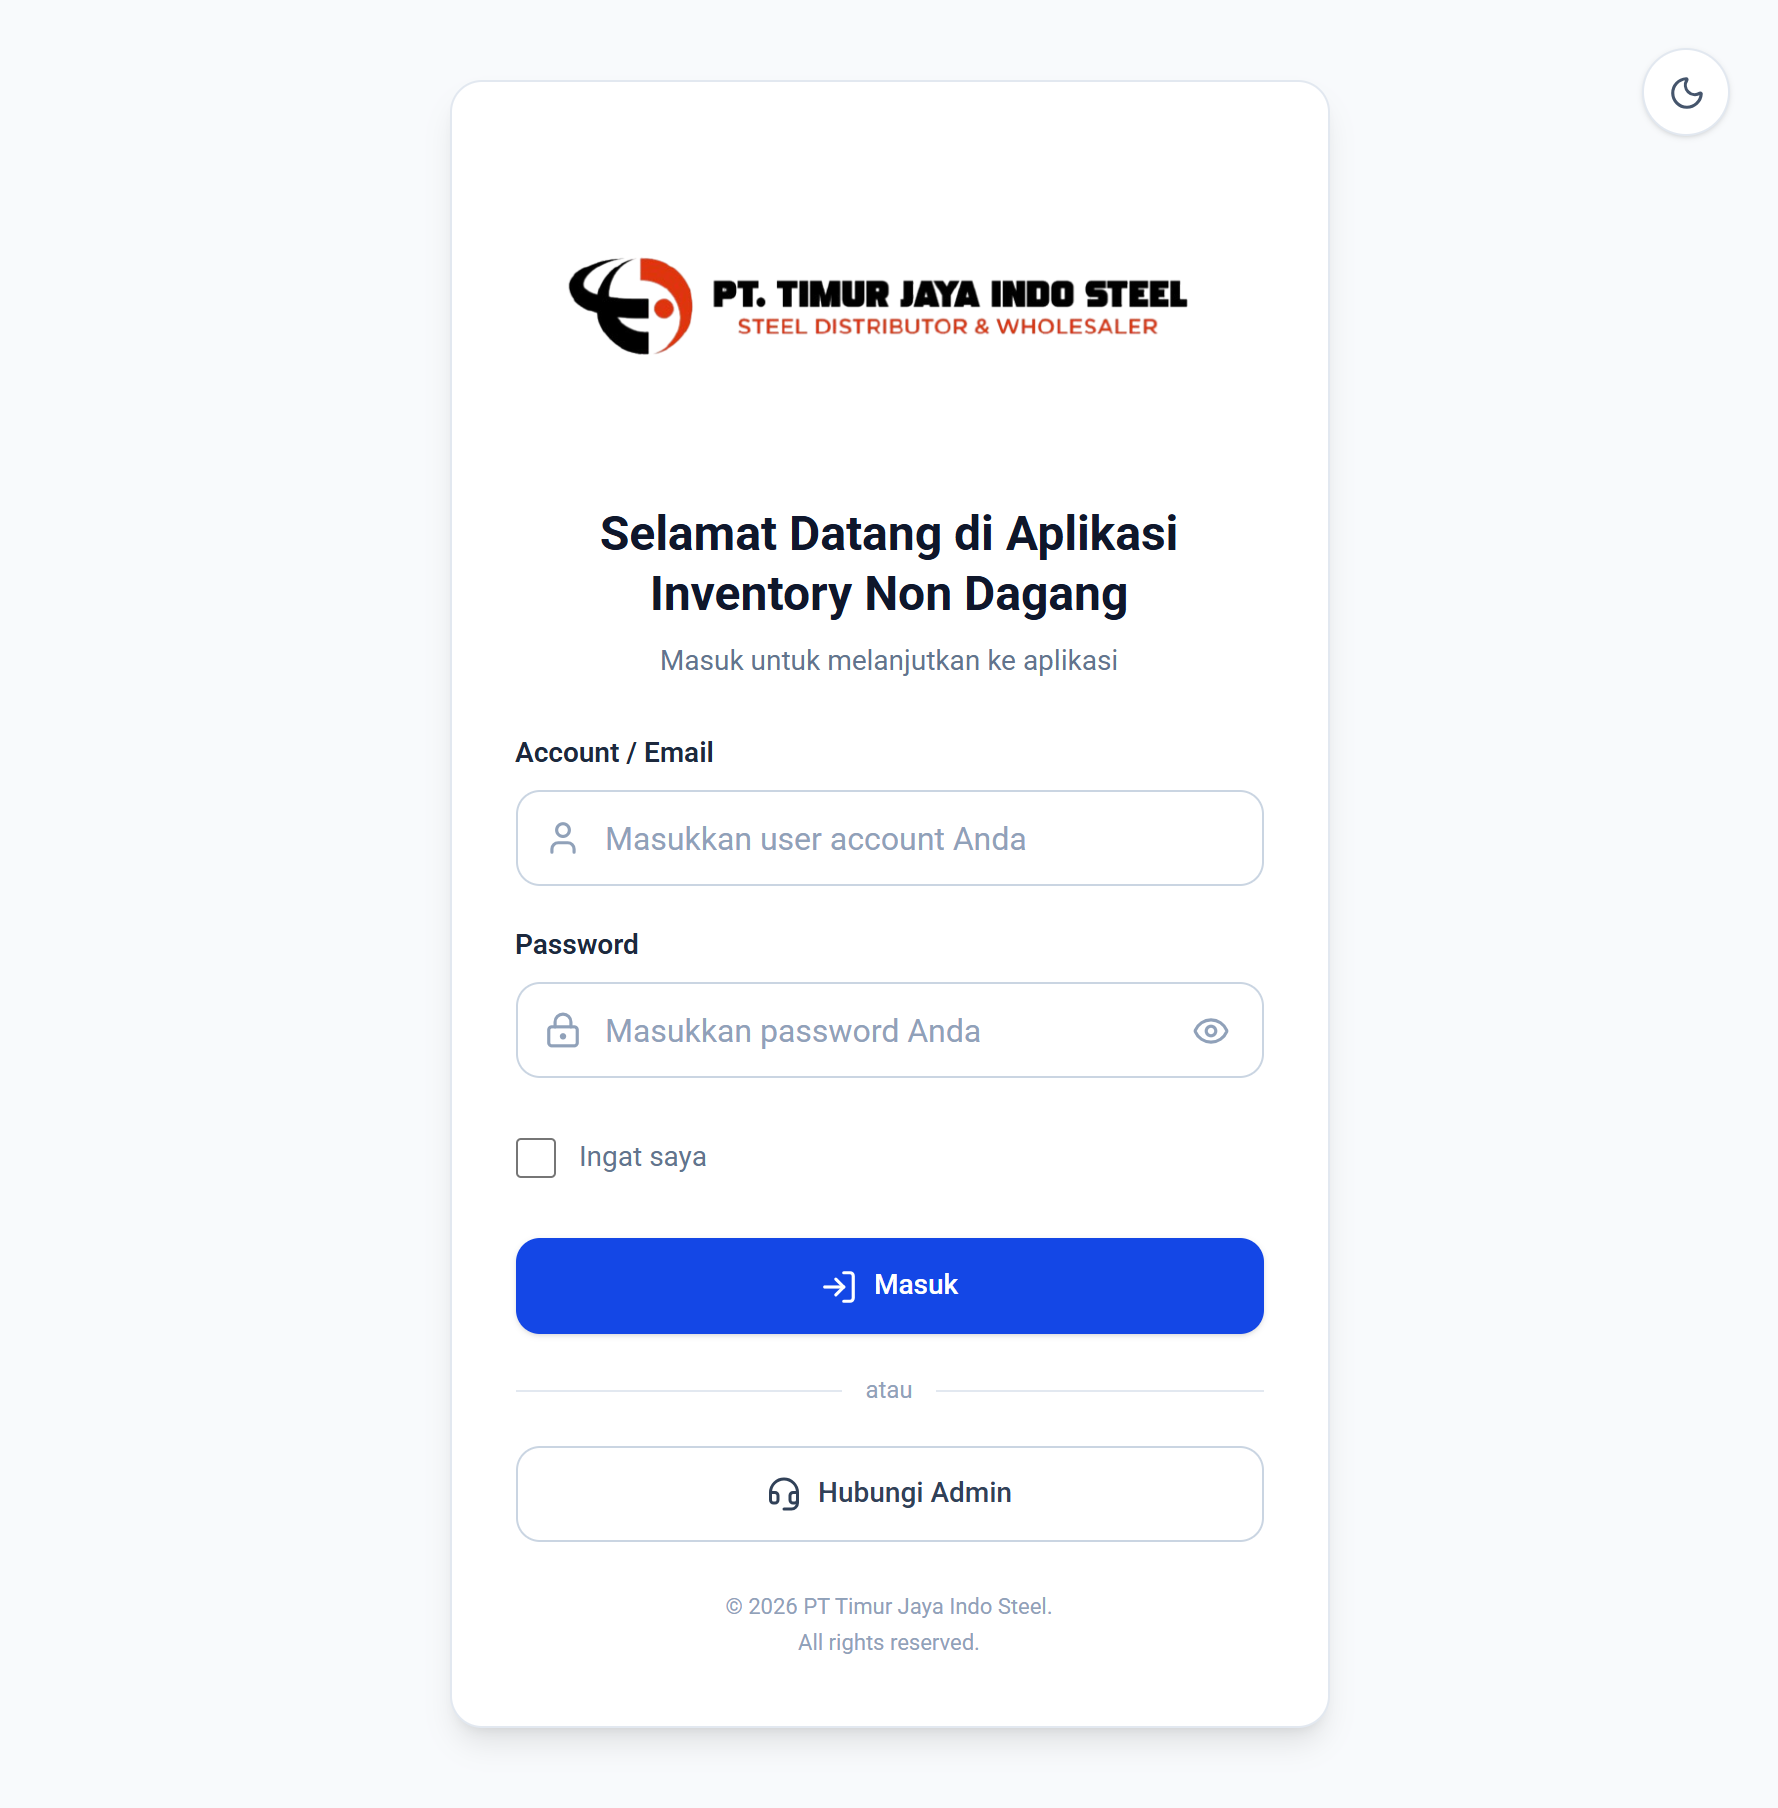
\includegraphics[
            width=0.72\linewidth,
            keepaspectratio
        ]{images/Login/login1.png}
    }

    \only<2>{
        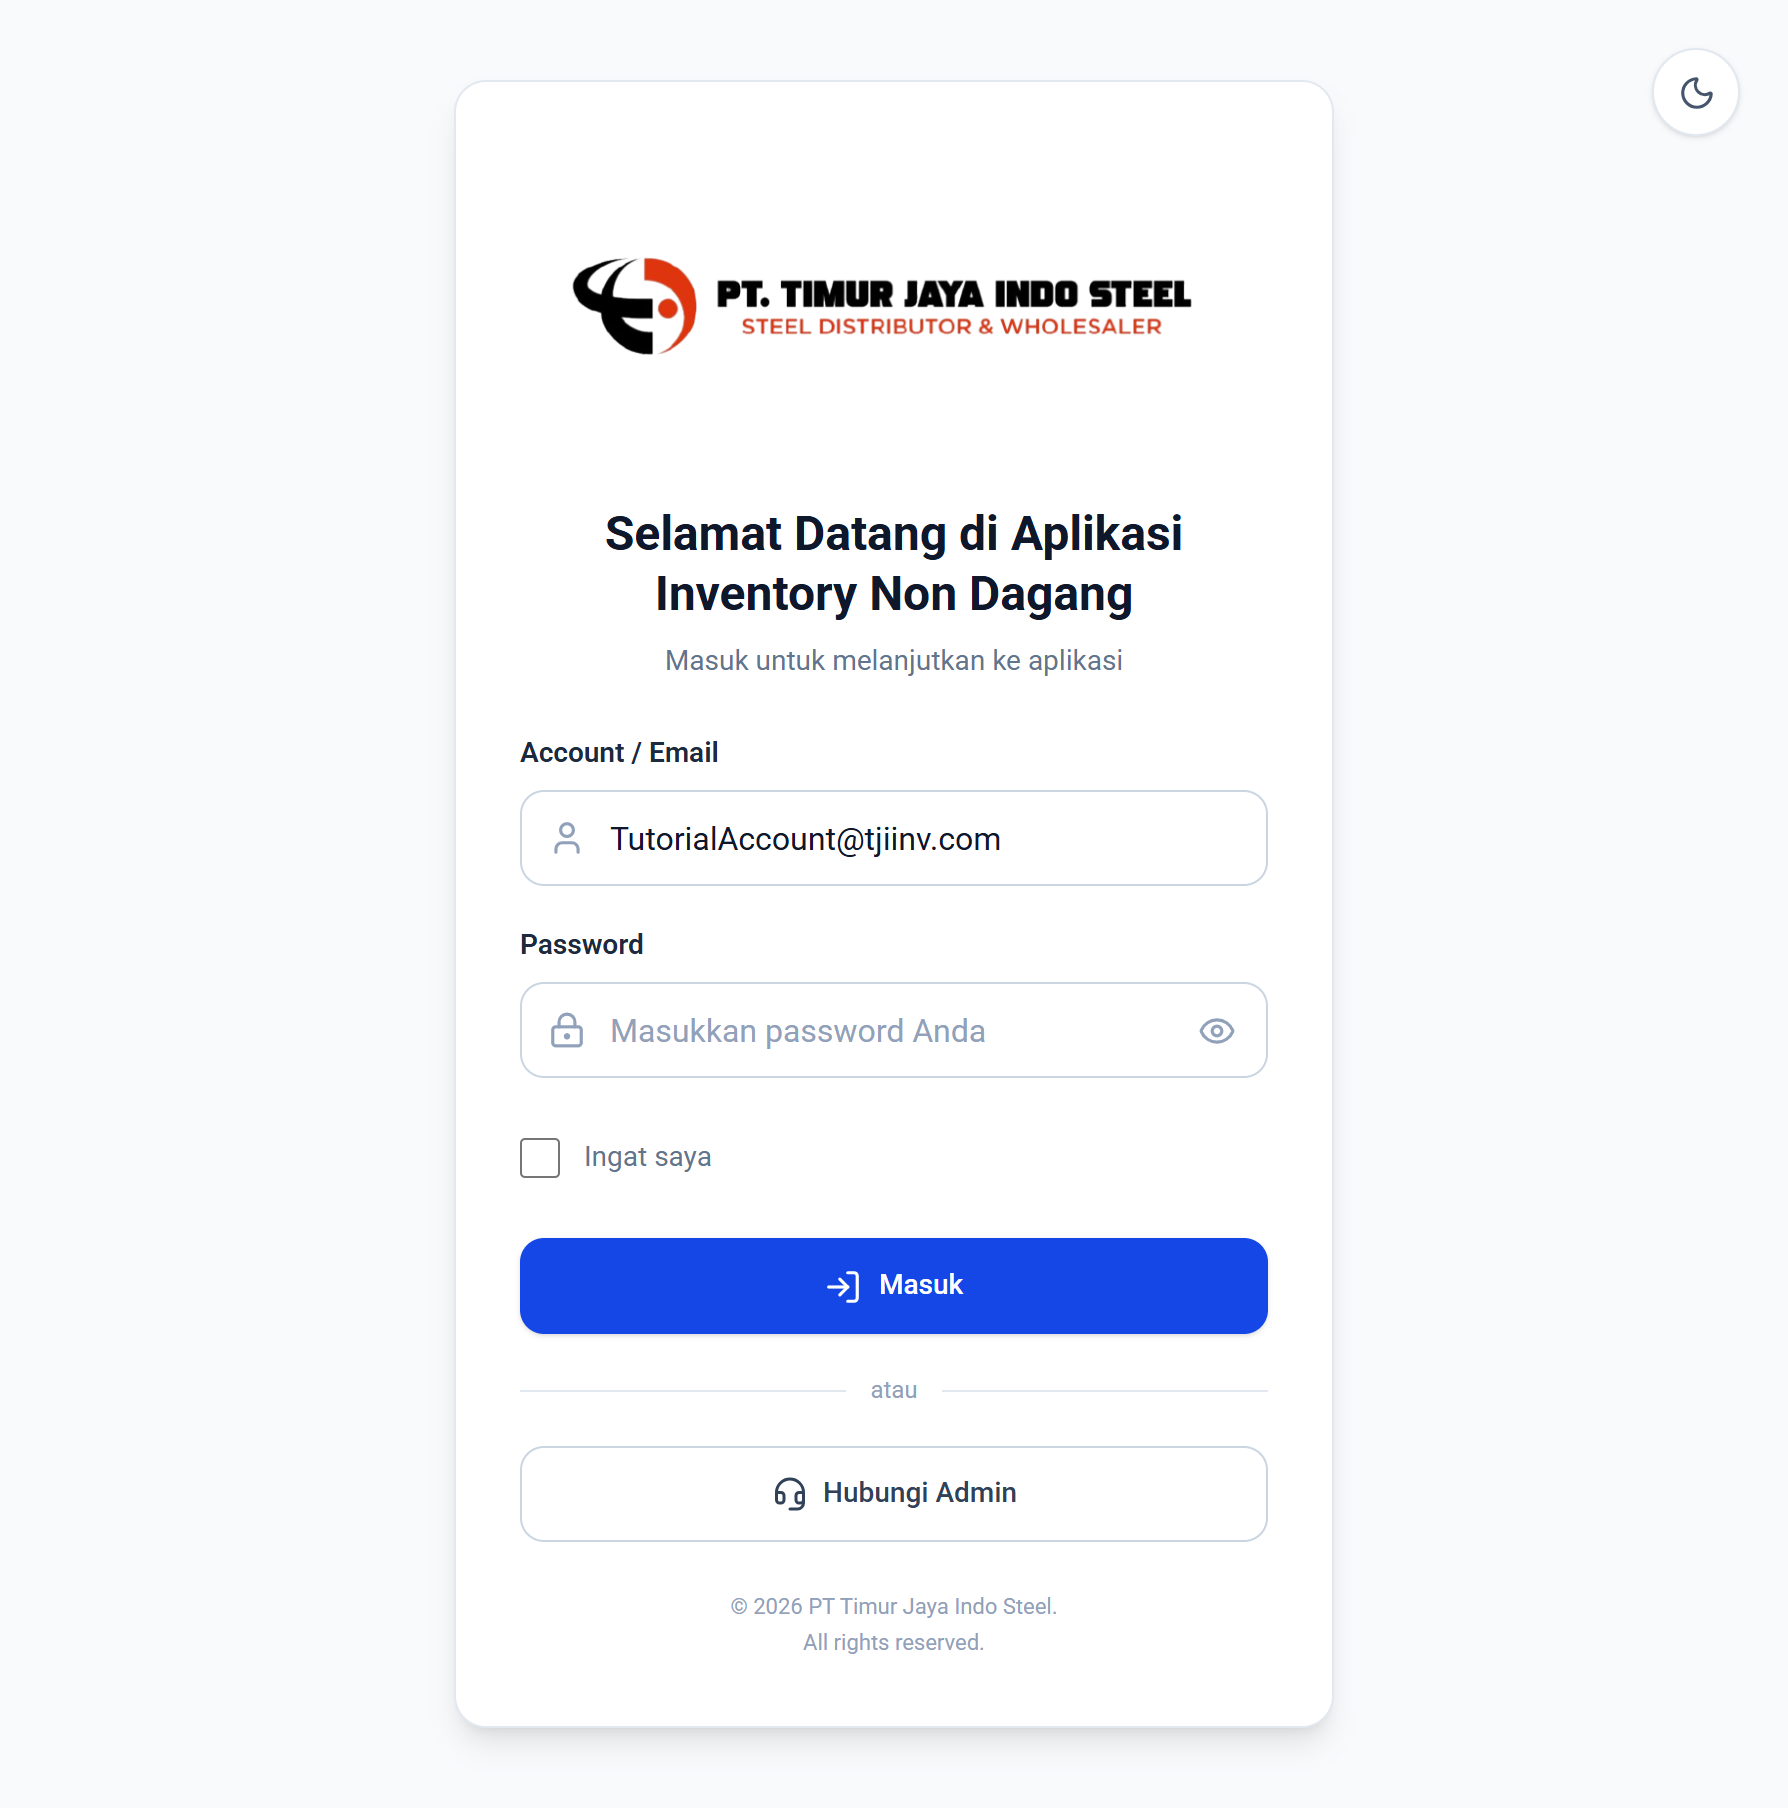
\includegraphics[
            width=0.72\linewidth,
            keepaspectratio
        ]{images/Login/login2.png}
    }

    \only<3>{
        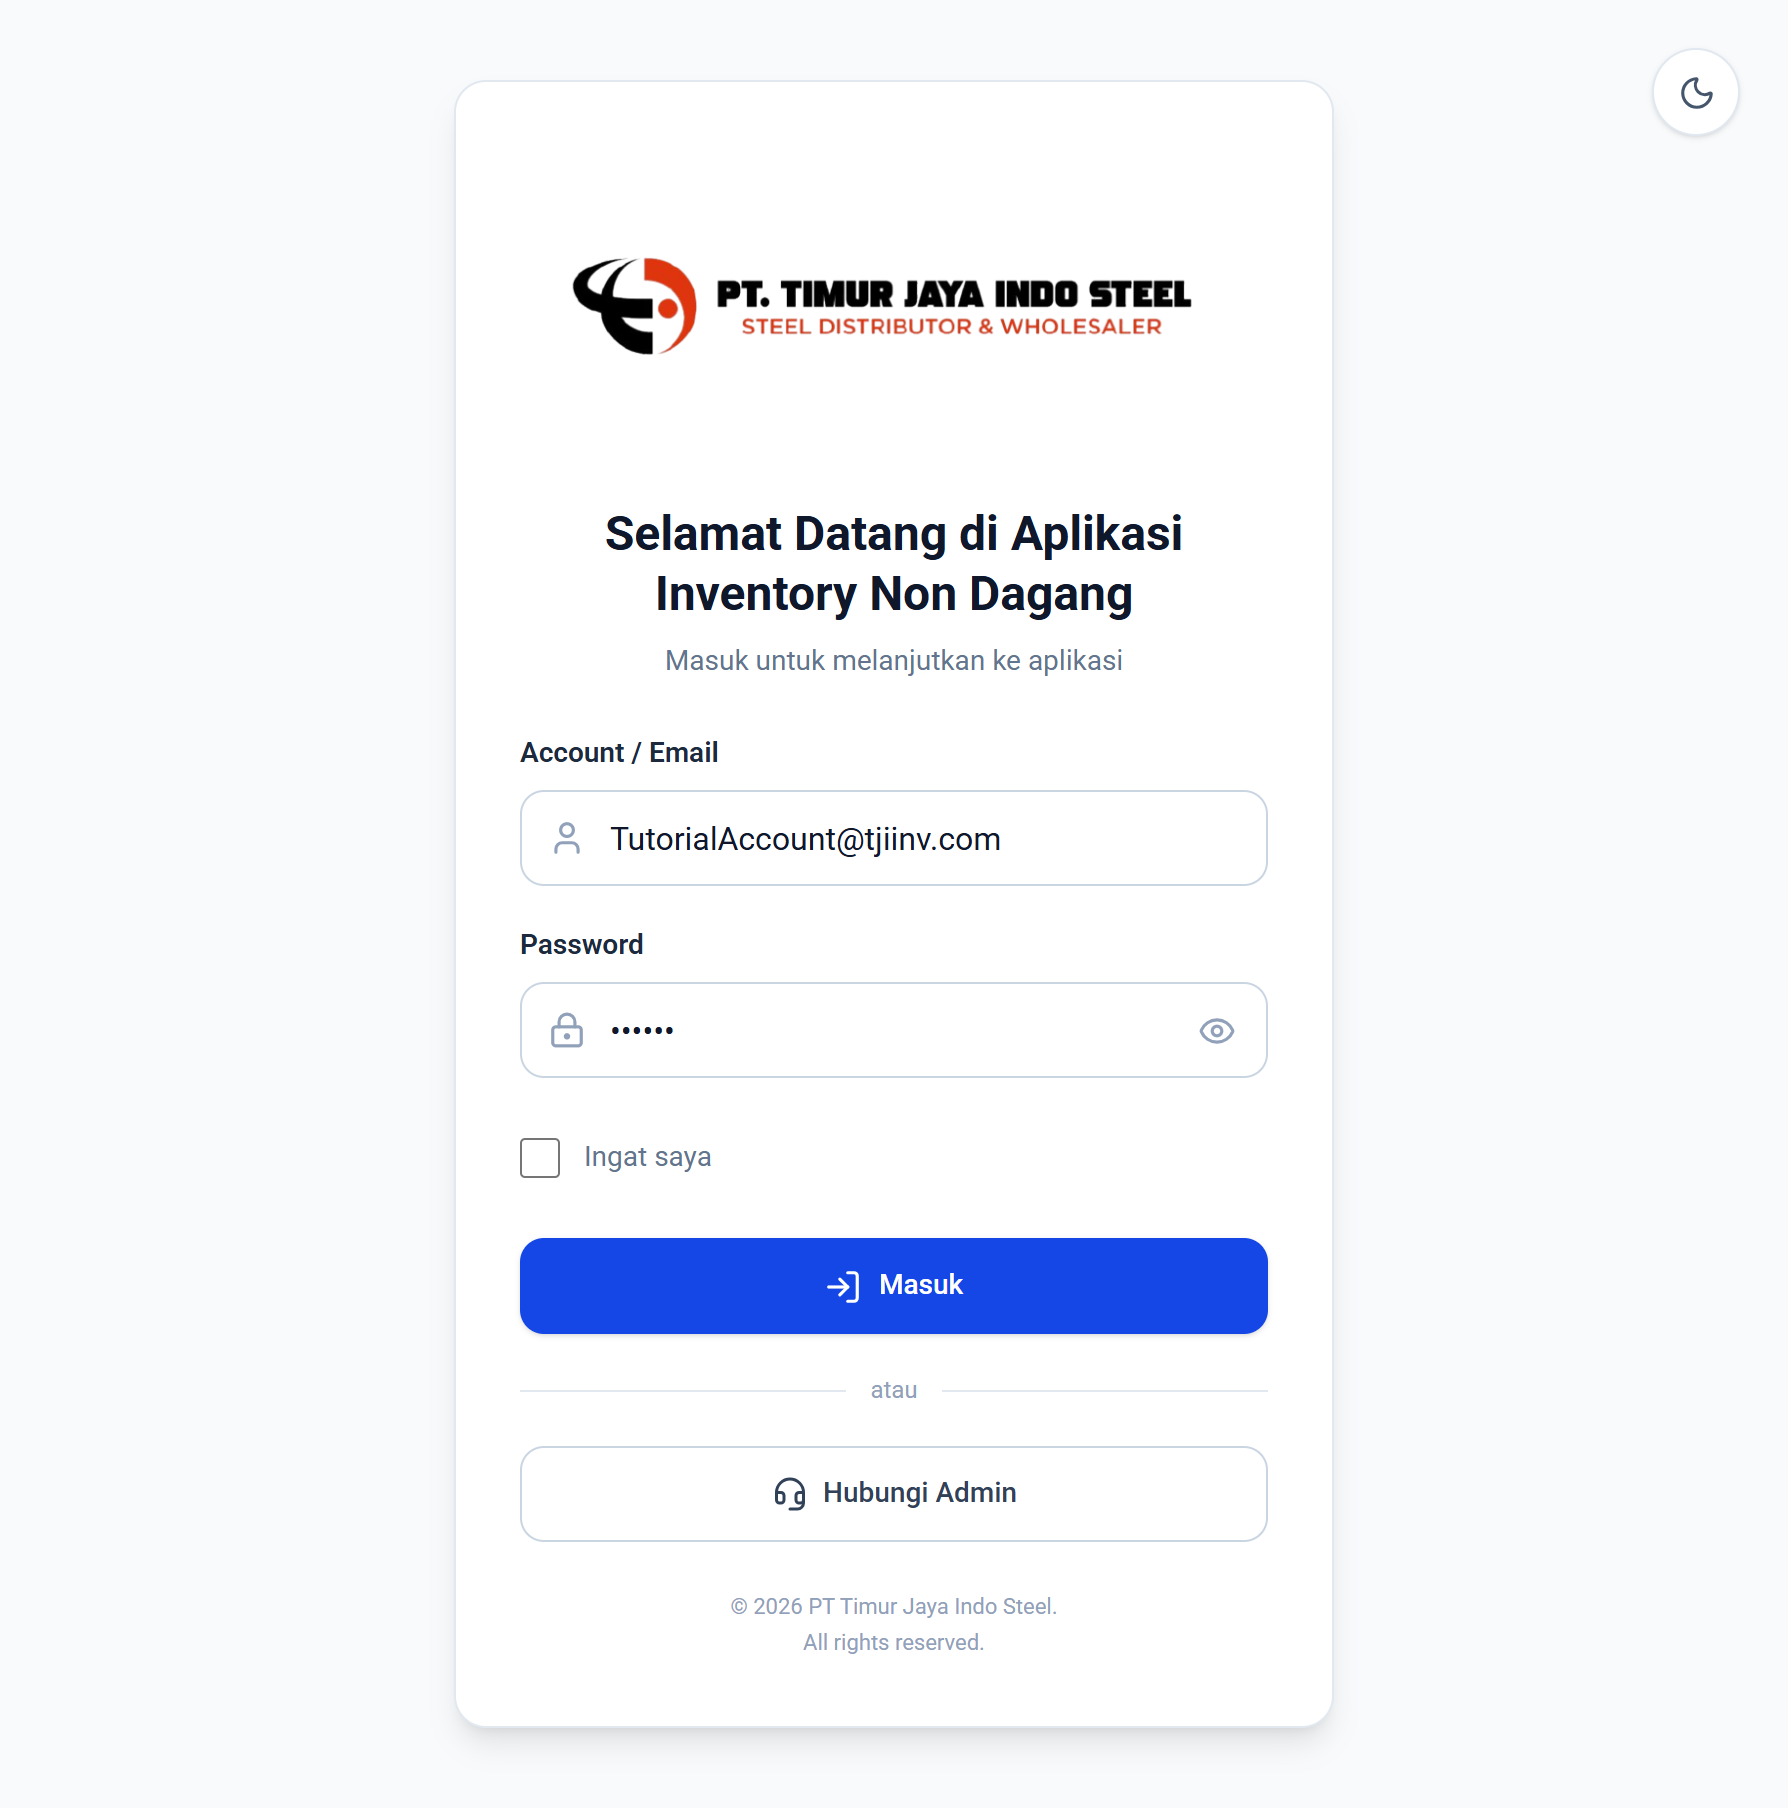
\includegraphics[
            width=0.72\linewidth,
            keepaspectratio
        ]{images/Login/login3.png}
    }

    \only<4>{
        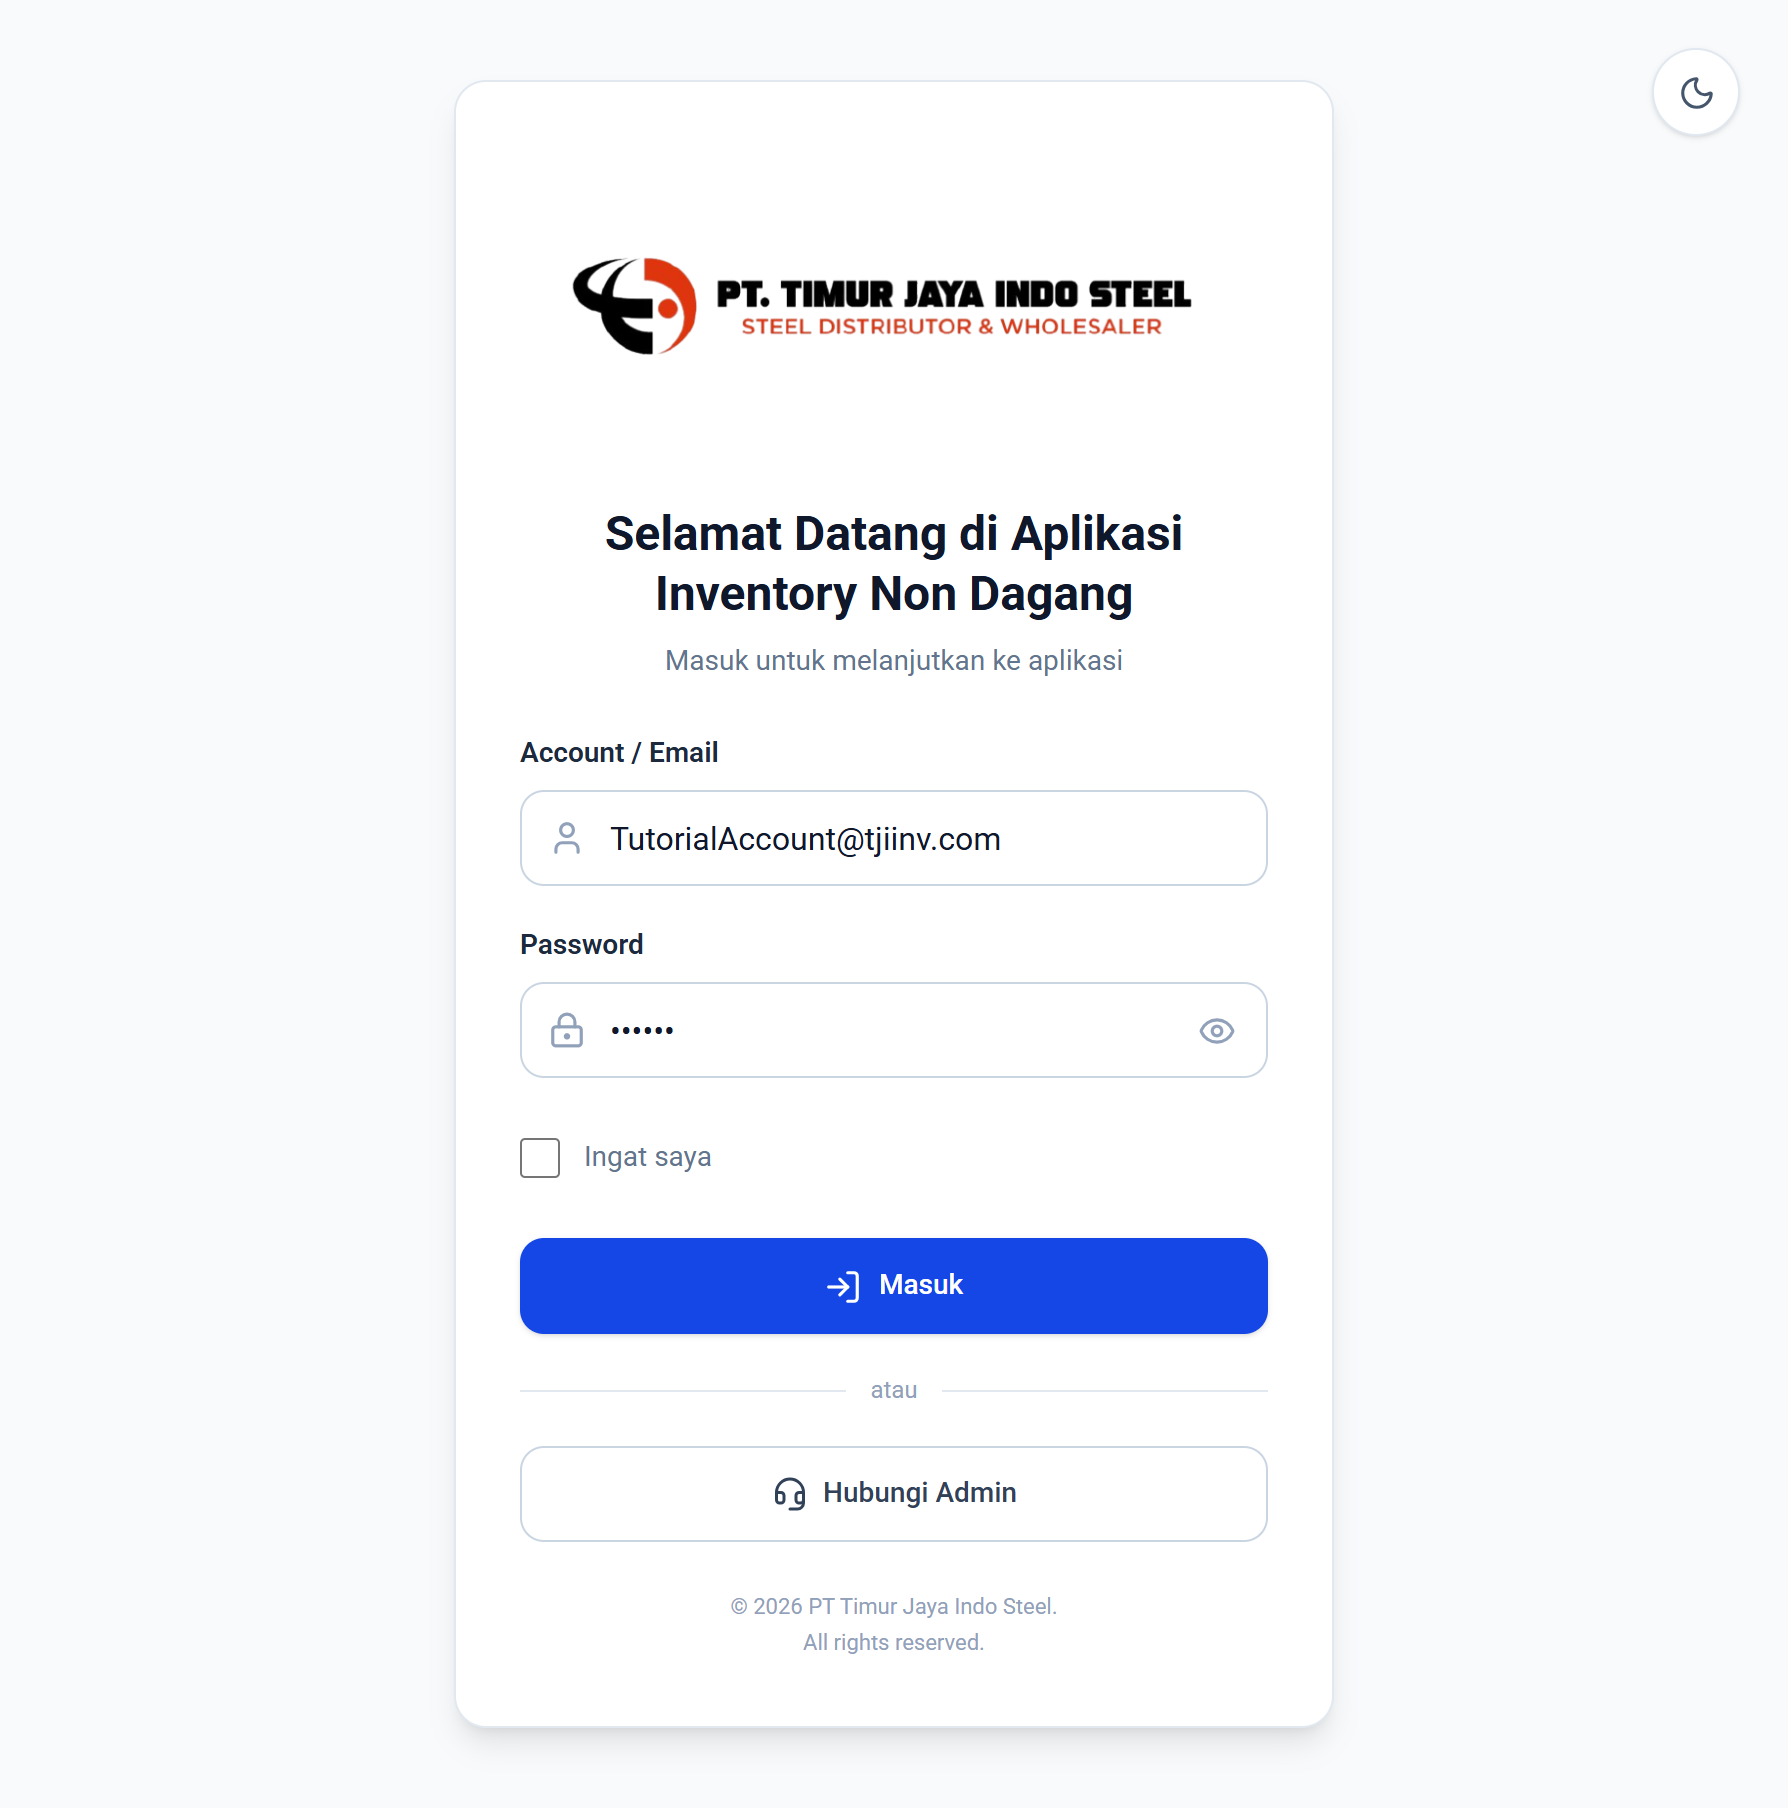
\includegraphics[
            width=0.72\linewidth,
            keepaspectratio
        ]{images/Login/login3.png}
    }
};

\highlight{1}{1.25cm}{2.55cm}{4.0cm}{0.65cm}
\highlight{2}{1.25cm}{1.85cm}{4.0cm}{0.65cm}
\highlight{3}{2.0cm}{0.75cm}{2.7cm}{0.65cm}
\successhighlight{4}{0.2cm}{0.2cm}{6.0cm}{3.5cm}

\end{tikzpicture}

\end{center}

% GAP
\column{0.025\textwidth}

% INSTRUCTION
\column{0.325\textwidth}

\stepcounterdisplay{1}{4}
\stepcounterdisplay{2}{4}
\stepcounterdisplay{3}{4}
\stepcounterdisplay{4}{4}

\vspace{0.02cm}

\sectionlabel{Langkah}

\vspace{0.10cm}

\stepitem{1}{1}{
Buka aplikasi Inventory Non Dagang di URL
\texttt{\fontsize{12}{14}\selectfont
http://172.16.0.193:5173/login}
}

\vspace{\TutorialGap}

\stepitem{2}{2}{
Masukkan username.
}

\vspace{\TutorialGap}

\stepitem{3}{3}{
Masukkan password.
}

\vspace{\TutorialGap}

\stepitem{4}{4}{
Klik \textbf{Masuk}.
}

\vspace{0.15cm}

\warningbox{Perhatian}{
Pastikan username dan password sesuai dengan
akun yang diberikan administrator.
}

\end{columns}

\end{frame}

% =========================================================
% DASHBOARD
% =========================================================

\begin{frame}{02 --- Dashboard}

\vspace{-0.25cm}

\begin{columns}[T,totalwidth=\textwidth]

% SCREENSHOT
\column{0.65\textwidth}

\begin{center}

\begin{tikzpicture}

\node[
    inner sep=0,
    outer sep=0
] (screen)
{
    \only<1>{
        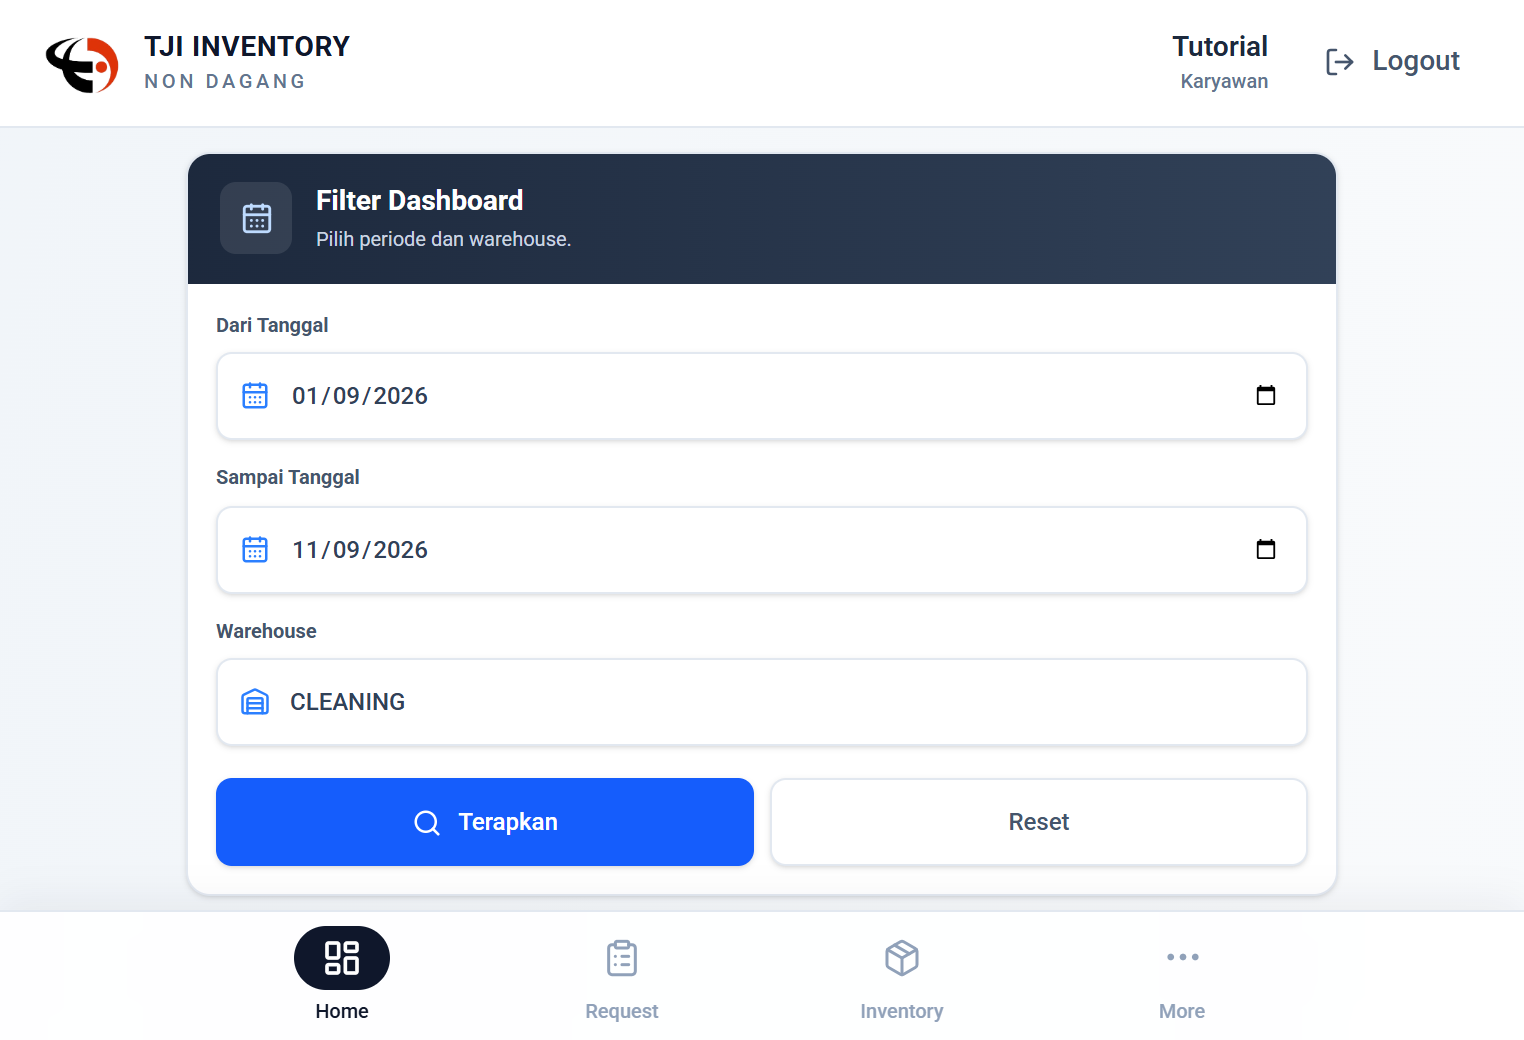
\includegraphics[
            width=0.8\linewidth,
            keepaspectratio
        ]{images/Dashboard/Dashboard1.png}
    }

    \only<2>{
        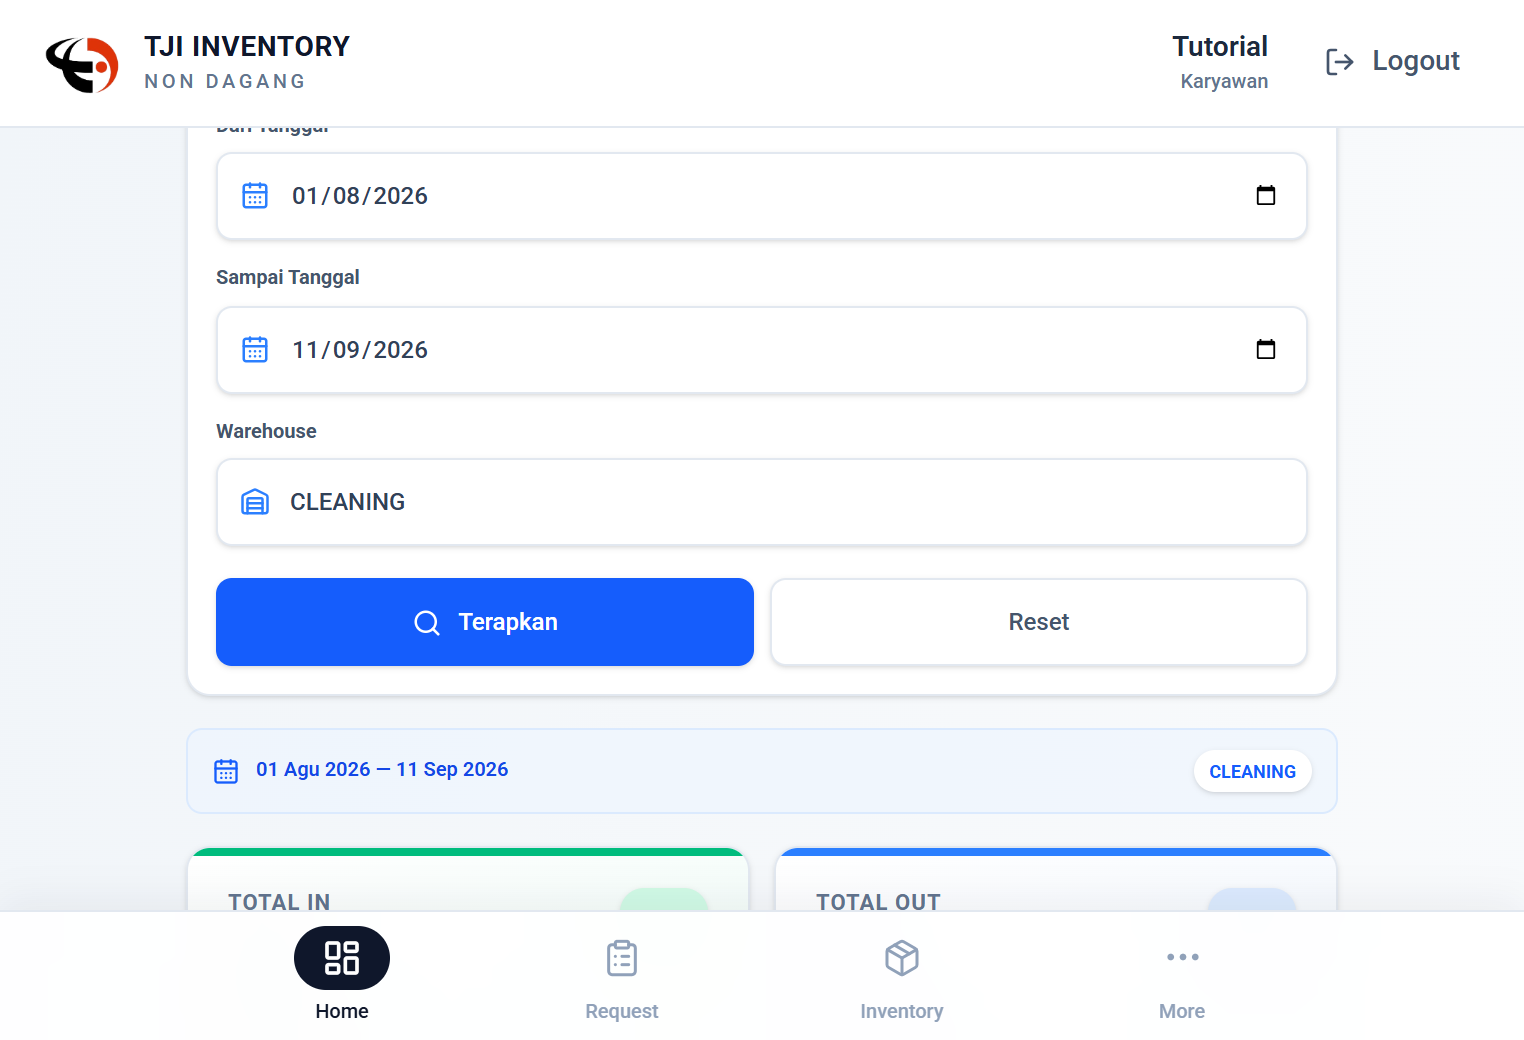
\includegraphics[
            width=0.8\linewidth,
            keepaspectratio
        ]{images/Dashboard/Dashboard2.png}
    }

    \only<3>{
        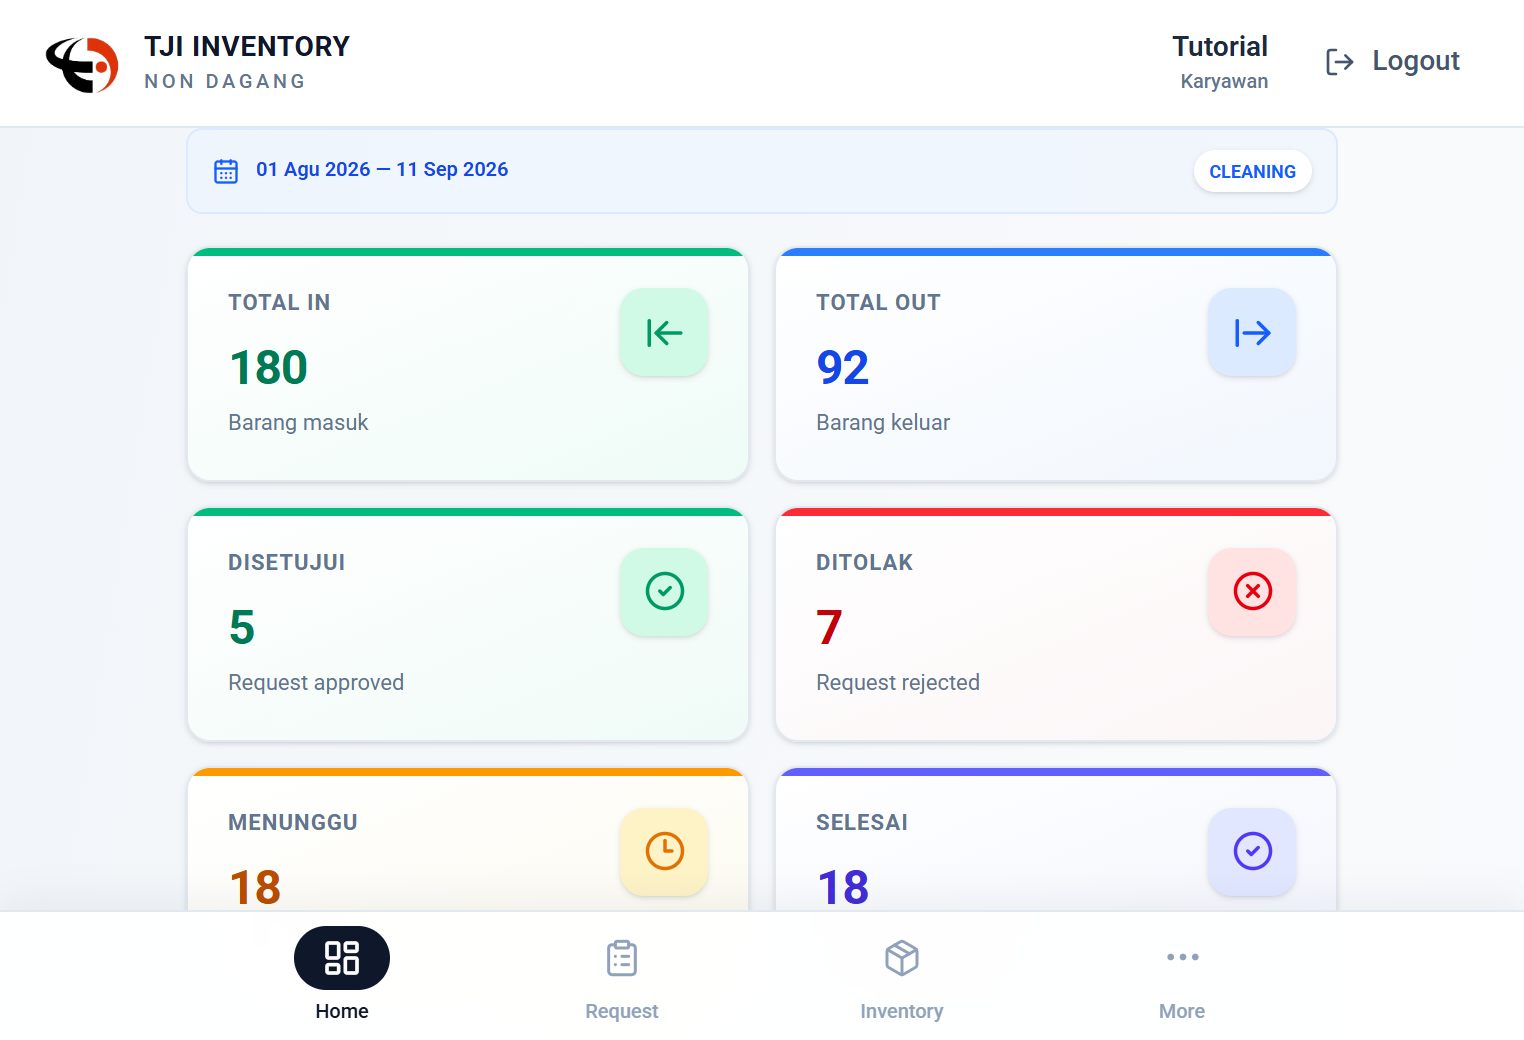
\includegraphics[
            width=0.8\linewidth,
            keepaspectratio
        ]{images/Dashboard/Dashboard3.png}
    }

    \only<4>{
        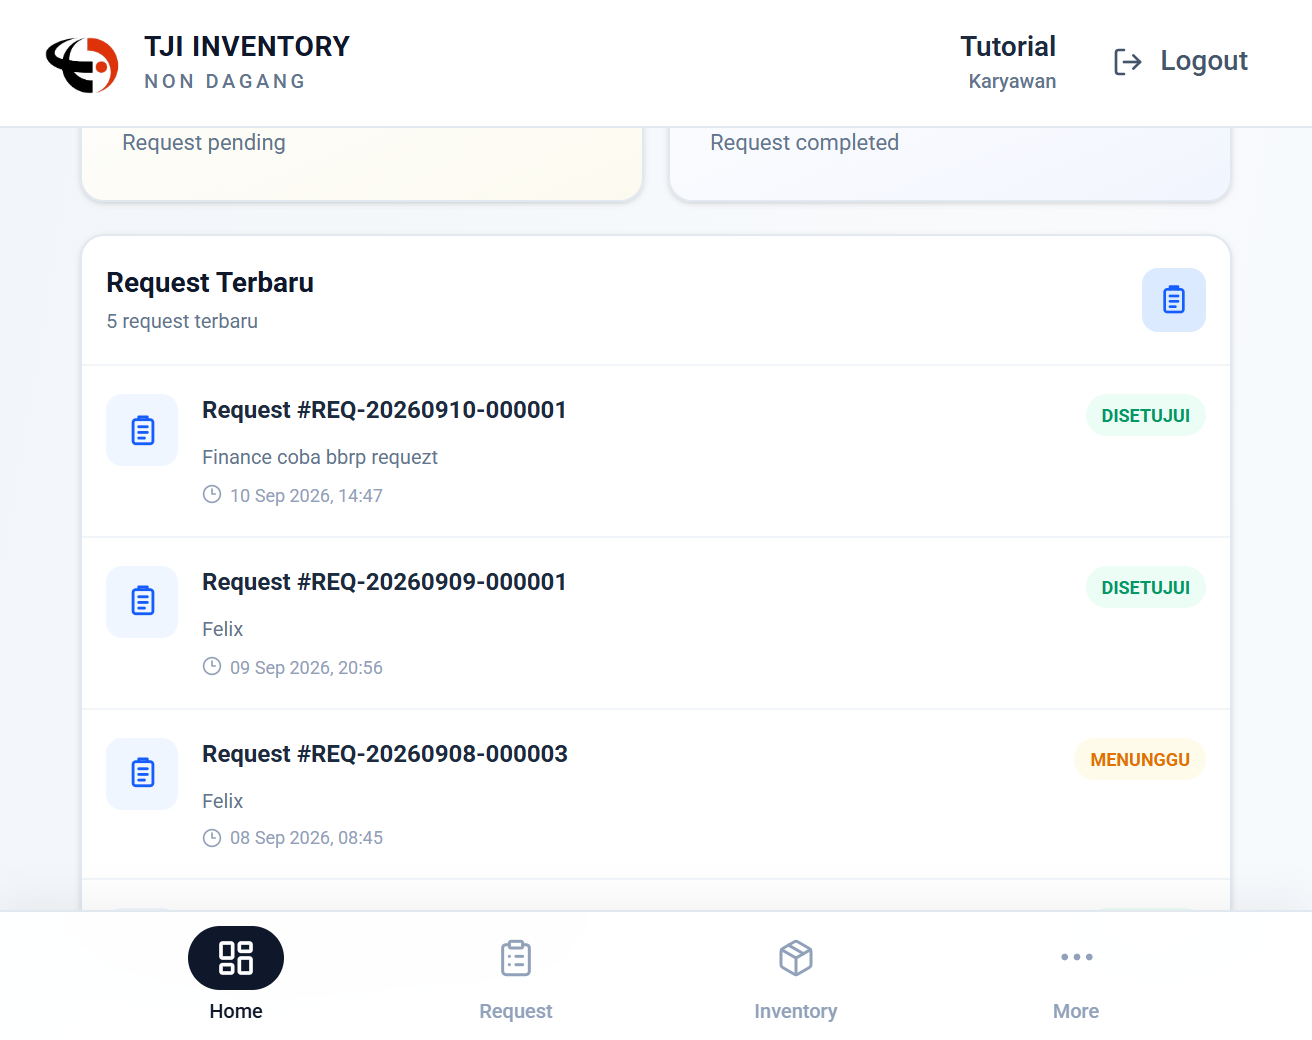
\includegraphics[
            width=0.72\linewidth,
            keepaspectratio
        ]{images/Dashboard/Dashboard4.png}
    }
};

\highlight{1}{1.25cm}{2.55cm}{4.0cm}{0.65cm}
\highlight{2}{1.25cm}{1.85cm}{4.0cm}{0.65cm}
\highlight{3}{2.0cm}{0.75cm}{2.7cm}{0.65cm}
\successhighlight{4}{0.2cm}{0.2cm}{6.0cm}{3.5cm}

\end{tikzpicture}

\end{center}

% GAP
\column{0.025\textwidth}

% INSTRUCTION
\column{0.325\textwidth}

\stepcounterdisplay{1}{4}
\stepcounterdisplay{2}{4}
\stepcounterdisplay{3}{4}
\stepcounterdisplay{4}{4}


\vspace{0.02cm}


\sectionlabel{Langkah}

\vspace{0.10cm}

\stepitem{1}{1}{
	Setelah login, Anda akan diarahkan ke halaman Dashboard.
}

\vspace{\TutorialGap}

\stepitem{2}{2}{
	Pilih periode tanggal, lalu klik \textbf{Terapkan}.
}

\vspace{\TutorialGap}

\stepitem{3}{3}{
	Dashboard akan menampilkan statistik dan informasi sesuai periode yang dipilih.
}

\vspace{\TutorialGap}

\stepitem{4}{4}{
	Dashboard juga menampilkan 5 request terbaru dari seluruh pengguna. Setiap request dapat diklik untuk melihat detail permintaan.
}


\vspace{0.15cm}

\warningbox{Perhatian}{
	Statistik Dashboard (\textit{Total IN}, \textit{Total OUT}, \textit{Disetujui}, \textit{Ditolak}, \textit{Menunggu}, dan \textit{Selesai}) serta bagian \textit{5 Request Terbaru} dapat diklik untuk melihat informasi lebih lanjut.
}



\end{columns}

\end{frame}

% =========================================================
% REQUEST FLOW
% =========================================================

% =========================================================
% REQUEST FLOW
% =========================================================

\begin{frame}{Prosedur Permohonan}
	
	\vspace{-0.05cm}
	
	\sectionlabel{Alur Proses Request Secara Umum}
	
	\vspace{0.40cm}
	
	\begin{center}
		
		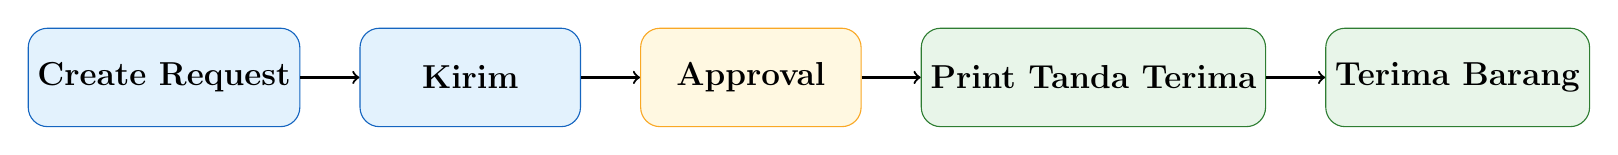
\begin{tikzpicture}[node distance=0.75cm]
			
			% ---------------------------------------------------------
			% STEP 1
			% ---------------------------------------------------------
			
			\node[
			draw=Primary,
			fill=Secondary,
			rounded corners=7pt,
			minimum width=2.8cm,
			minimum height=1.25cm,
			align=center,
			font=\large
			]
			(request)
			{\textbf{Create Request}};
			
			% ---------------------------------------------------------
			% STEP 2
			% ---------------------------------------------------------
			
			\node[
			draw=Primary,
			fill=Secondary,
			rounded corners=7pt,
			minimum width=2.8cm,
			minimum height=1.25cm,
			align=center,
			font=\large,
			right=of request
			]
			(submit)
			{\textbf{Kirim}};
			
			% ---------------------------------------------------------
			% STEP 3
			% ---------------------------------------------------------
			
			\node[
			draw=Warning,
			fill=WarningLight,
			rounded corners=7pt,
			minimum width=2.8cm,
			minimum height=1.25cm,
			align=center,
			font=\large,
			right=of submit
			]
			(approve)
			{\textbf{Approval}};
			
			% ---------------------------------------------------------
			% STEP 4
			% ---------------------------------------------------------
			
			\node[
			draw=Success,
			fill=SuccessLight,
			rounded corners=7pt,
			minimum width=2.8cm,
			minimum height=1.25cm,
			align=center,
			font=\large,
			right=of approve
			]
			(ptt)
			{\textbf{Print Tanda Terima}};
			
			% ---------------------------------------------------------
			% STEP 5
			% ---------------------------------------------------------
			
			\node[
			draw=Success,
			fill=SuccessLight,
			rounded corners=7pt,
			minimum width=2.8cm,
			minimum height=1.25cm,
			align=center,
			font=\large,
			right=of ptt
			]
			(receive)
			{\textbf{Terima Barang}};
			
			% ---------------------------------------------------------
			% ARROWS
			% ---------------------------------------------------------
			
			\draw[->,thick]
			(request) -- (submit);
			
			\draw[->,thick]
			(submit) -- (approve);
			
			\draw[->,thick]
			(approve) -- (ptt);
			
			\draw[->,thick]
			(ptt) -- (receive);
			
		\end{tikzpicture}
		
	\end{center}
	
	\vspace{0.50cm}
	
	% =========================================================
	% STEP 1
	% =========================================================
	
	\only<1>{
		\infobox{STEP 1 --- Create Request}{
			Pemohon membuat request barang sesuai dengan kebutuhan,
			lalu mengisikan data pada Form Aplikasi TJI Inventory Non-Dagang.
		}
	}
	
	% =========================================================
	% STEP 2
	% =========================================================
	
	\only<2>{
		\infobox{STEP 2 --- Kirim}{
			Request yang telah diisi lengkap dikirim untuk diproses.
		}
	}
	
	% =========================================================
	% STEP 3
	% =========================================================
	
	\only<3>{
		\infobox{STEP 3 --- Approval}{
			Request diperiksa dan disetujui oleh pihak yang
			memiliki hak approval.
		}
	}
	
	% =========================================================
	% STEP 4
	% =========================================================
	
	\only<4>{
		\infobox{STEP 4 --- Print Tanda Terima}{
			Setelah request disetujui (berstatus Disetujui) pemohon mencetak tanda terima sebagai bukti serah terima barang.
		}
	}
	
	% =========================================================
	% STEP 5
	% =========================================================
	
	\only<5>{
		\infobox{STEP 5 --- Terima Barang}{
			Pemohon menandatangani dan menyerahkan tanda terima, kemudian menerima barang dari petugas.
		}
	}
	
\end{frame}
% =========================================================
% CREATE REQUEST
% =========================================================

\begin{frame}{03.1 --- Membuat Request/Permohonan Barang Non Dagang}
	
	\vspace{-0.25cm}
	
	\begin{columns}[T,totalwidth=\textwidth]
		
		% =========================================================
		% SCREENSHOT
		% =========================================================
		
		\column{0.65\textwidth}
		
		\begin{center}
			
			\begin{tikzpicture}
				
				\node[
				inner sep=0,
				outer sep=0
				] (screen)
				{
					% -----------------------------------------------------
					% STEP 1
					% -----------------------------------------------------
					\only<1>{
						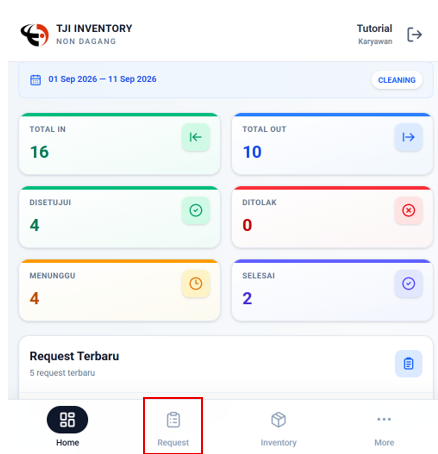
\includegraphics[
						width=0.5\linewidth,
						keepaspectratio
						]{images/Request/Request.png}
					}
					
					% -----------------------------------------------------
					% STEP 2
					% -----------------------------------------------------
					\only<2>{
						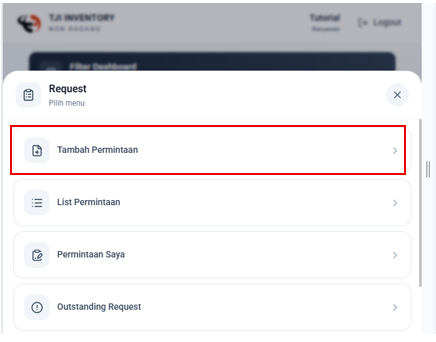
\includegraphics[
						width=0.8\linewidth,
						keepaspectratio
						]{images/Request/Request2.png}
					}
					
					% -----------------------------------------------------
					% STEP 3
					% -----------------------------------------------------
					\only<3>{
						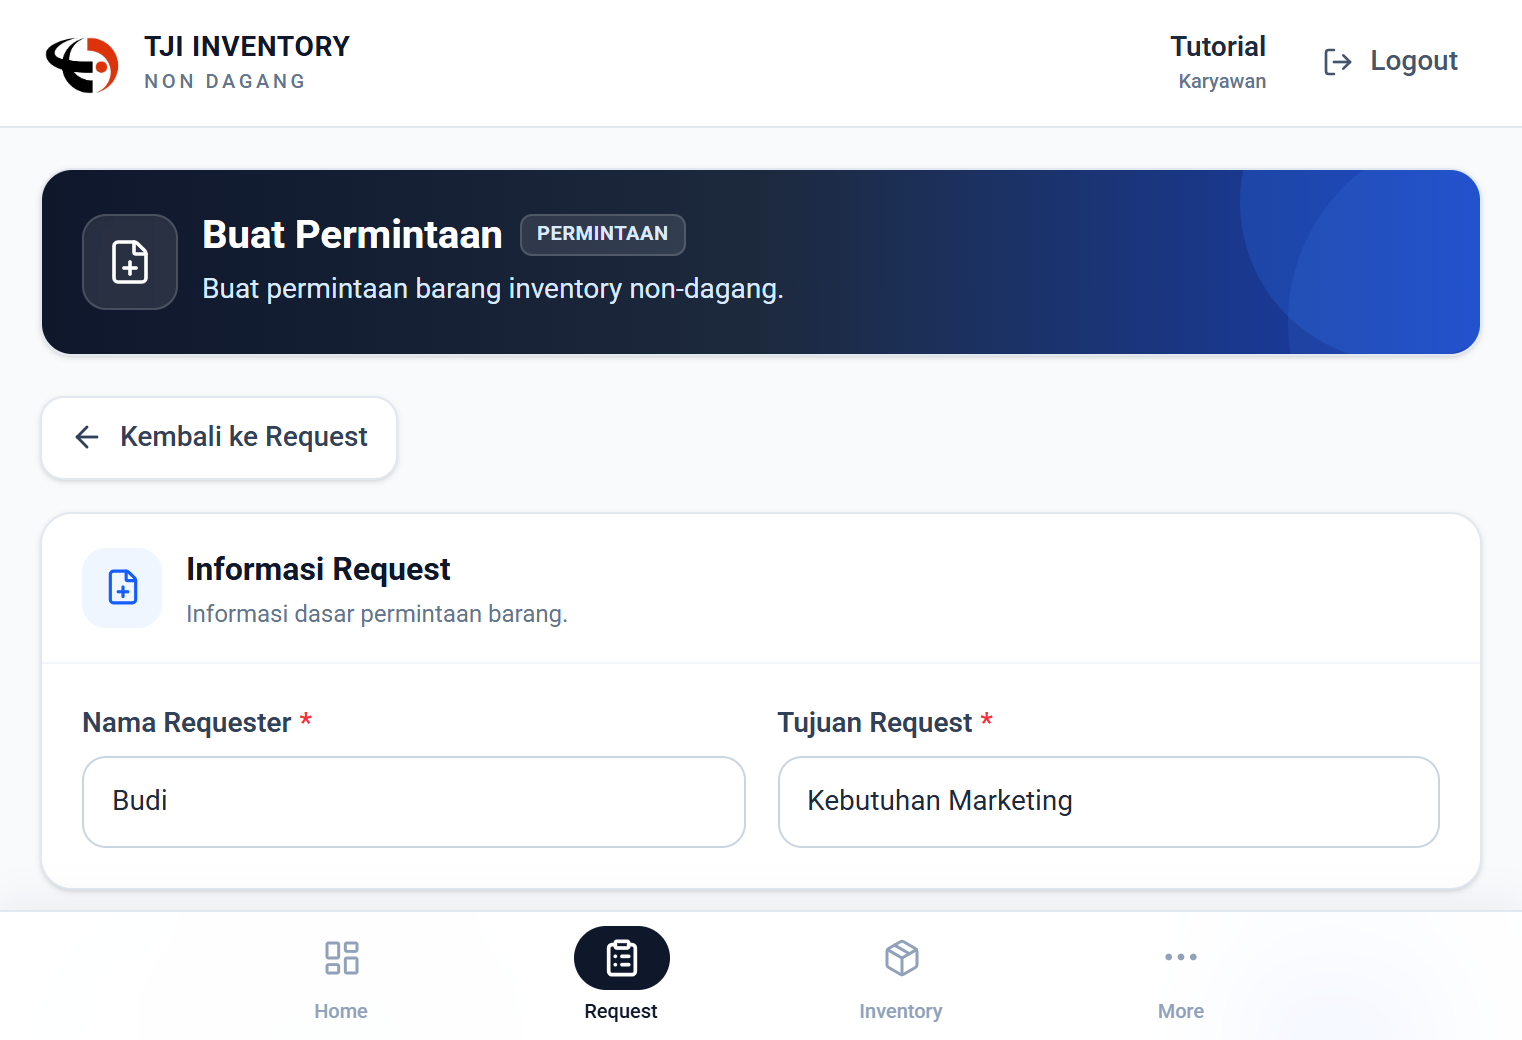
\includegraphics[
						width=0.8\linewidth,
						keepaspectratio
						]{images/Request/Request3.png}
					}
					
					% -----------------------------------------------------
					% STEP 4
					% -----------------------------------------------------
					\only<4>{
						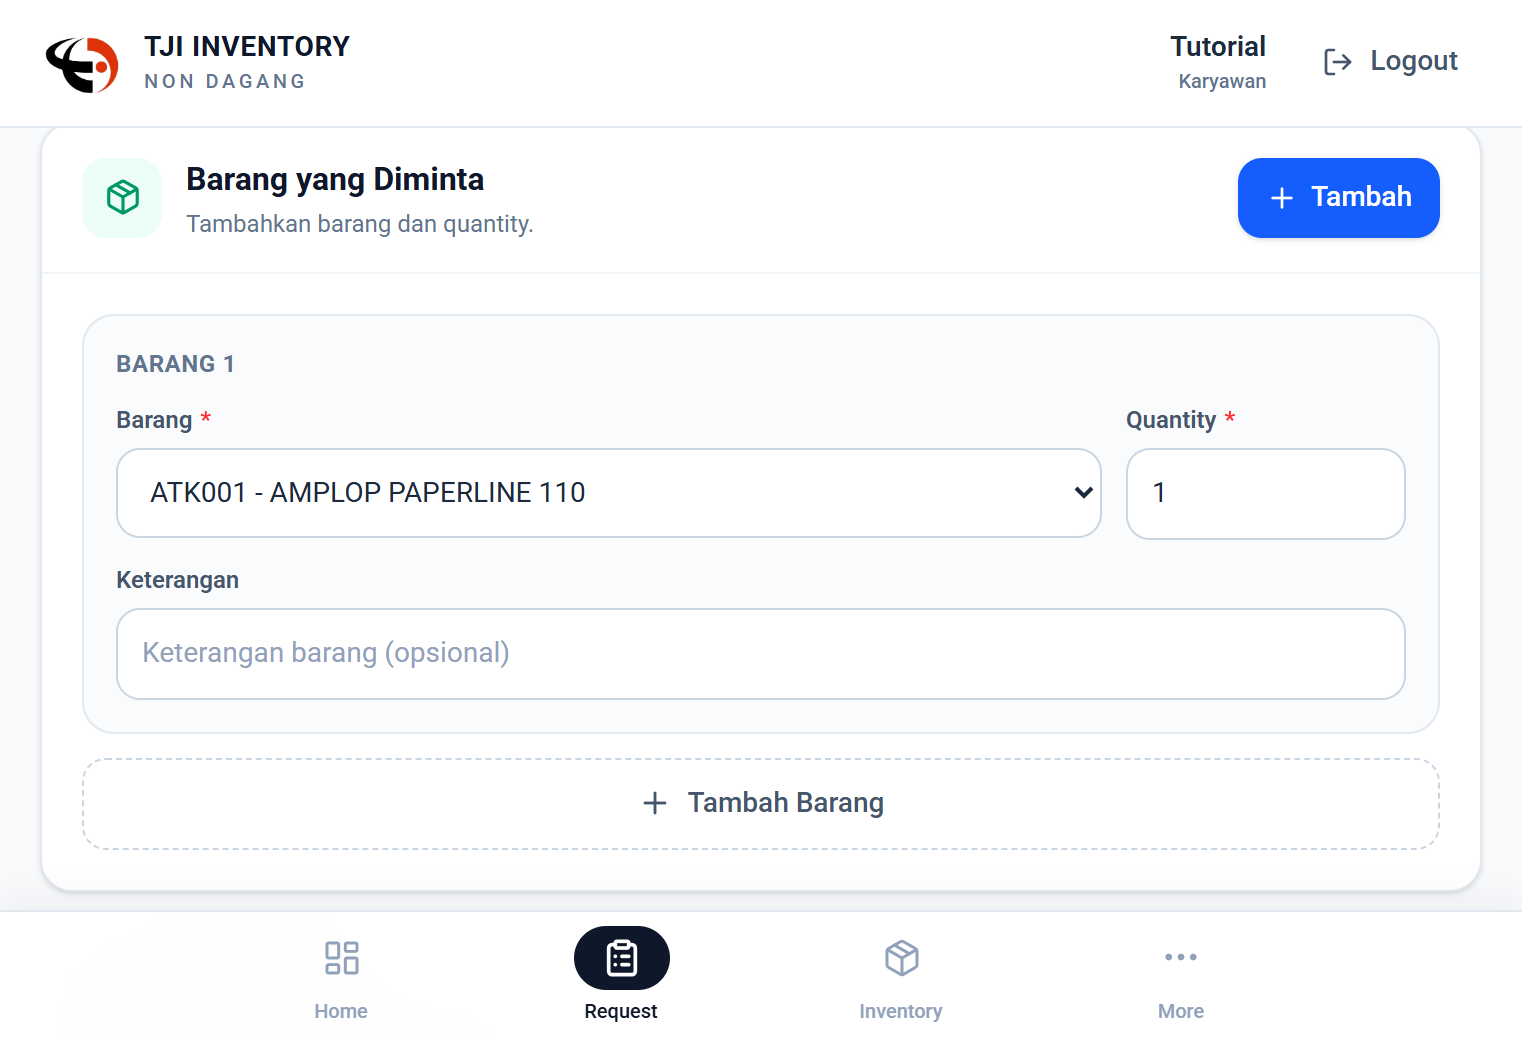
\includegraphics[
						width=0.8\linewidth,
						keepaspectratio
						]{images/Request/Request4.png}
					}
					
					% -----------------------------------------------------
					% STEP 5--10
					% -----------------------------------------------------
					\only<5>{
						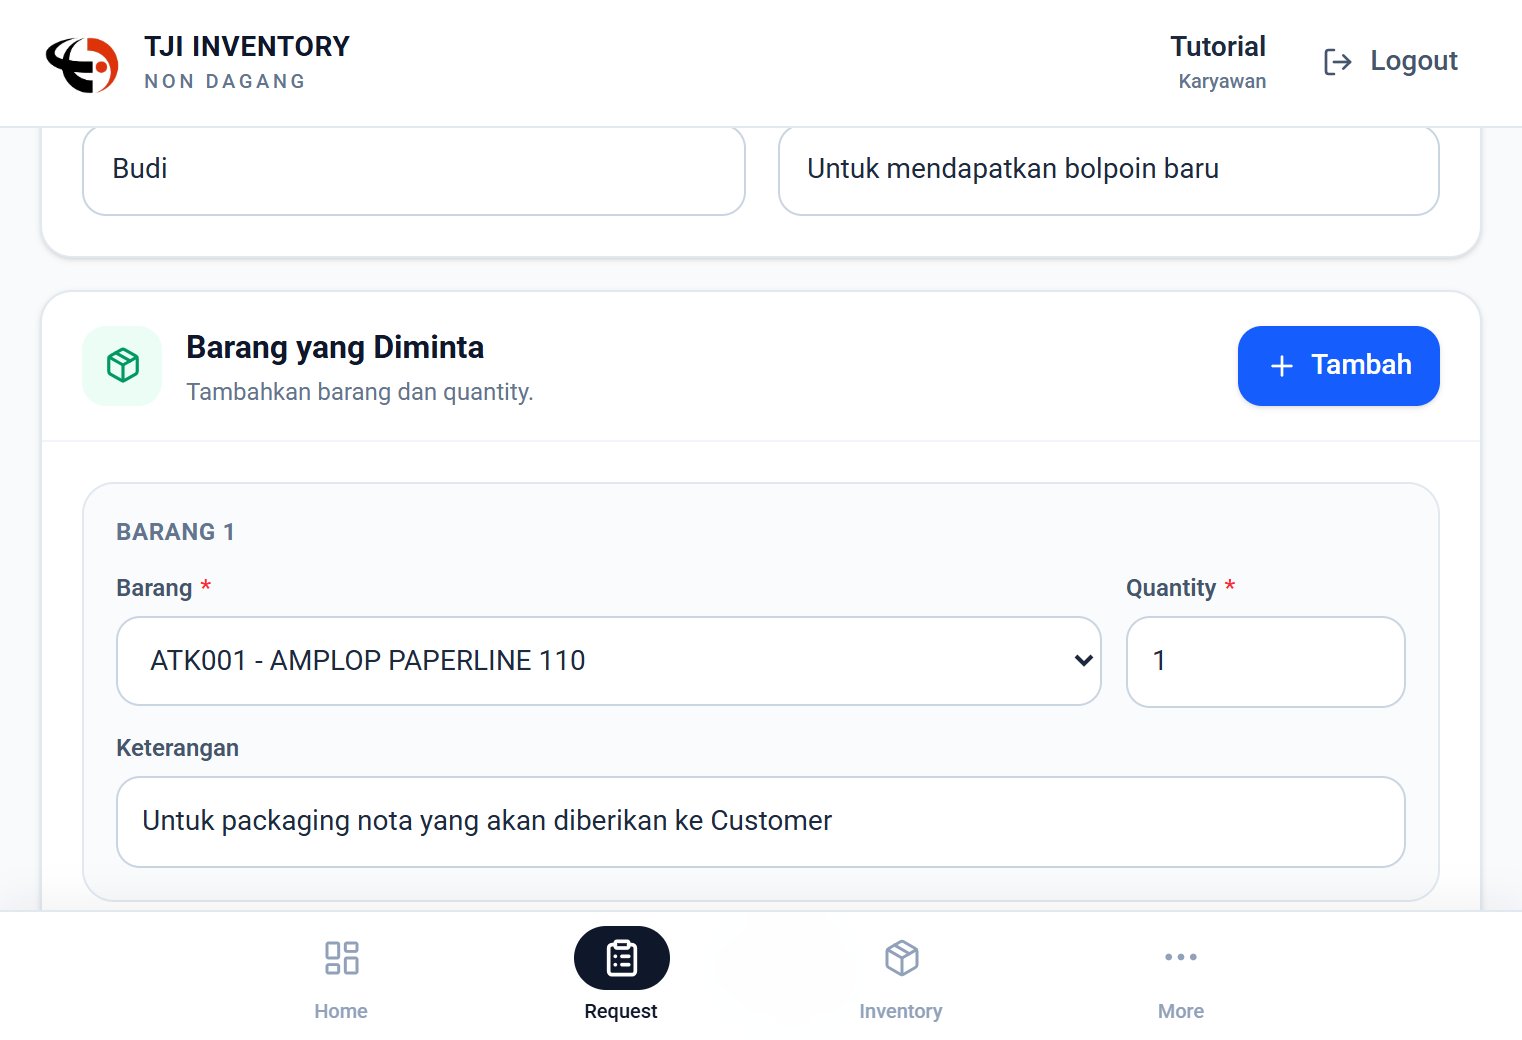
\includegraphics[
						width=0.8\linewidth,
						keepaspectratio
						]{images/Request/Request5.png}
					}
					\only<6>{
						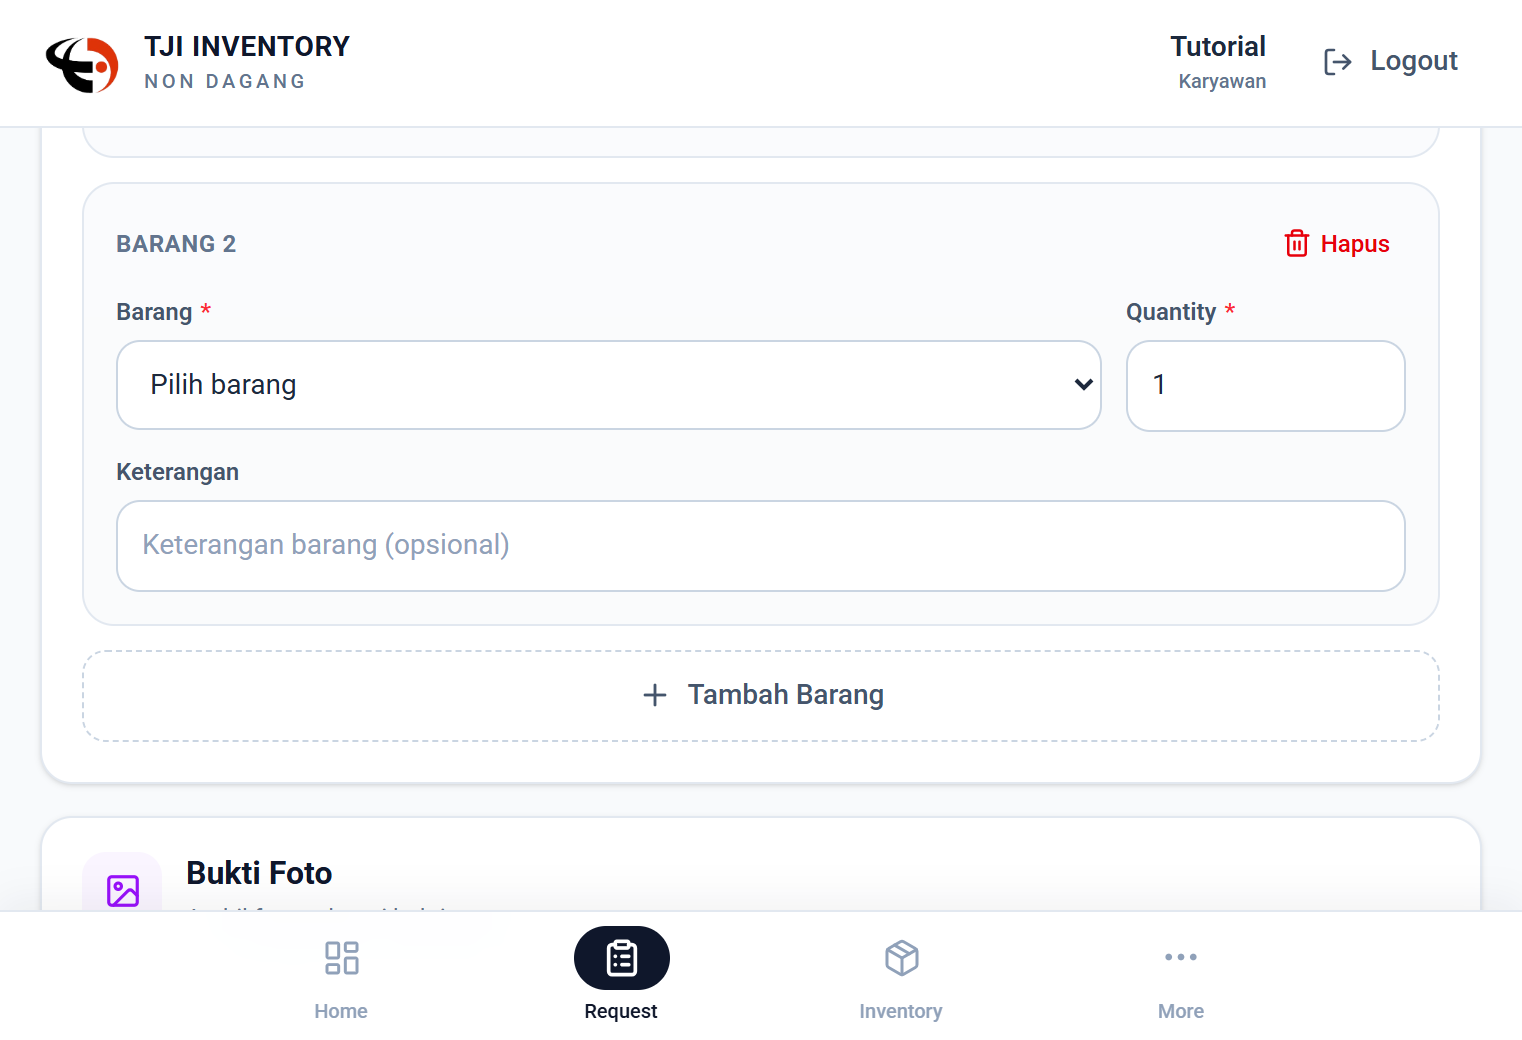
\includegraphics[
						width=0.8\linewidth,
						keepaspectratio
						]{images/Request/Request7.png}
					}
					\only<7>{
						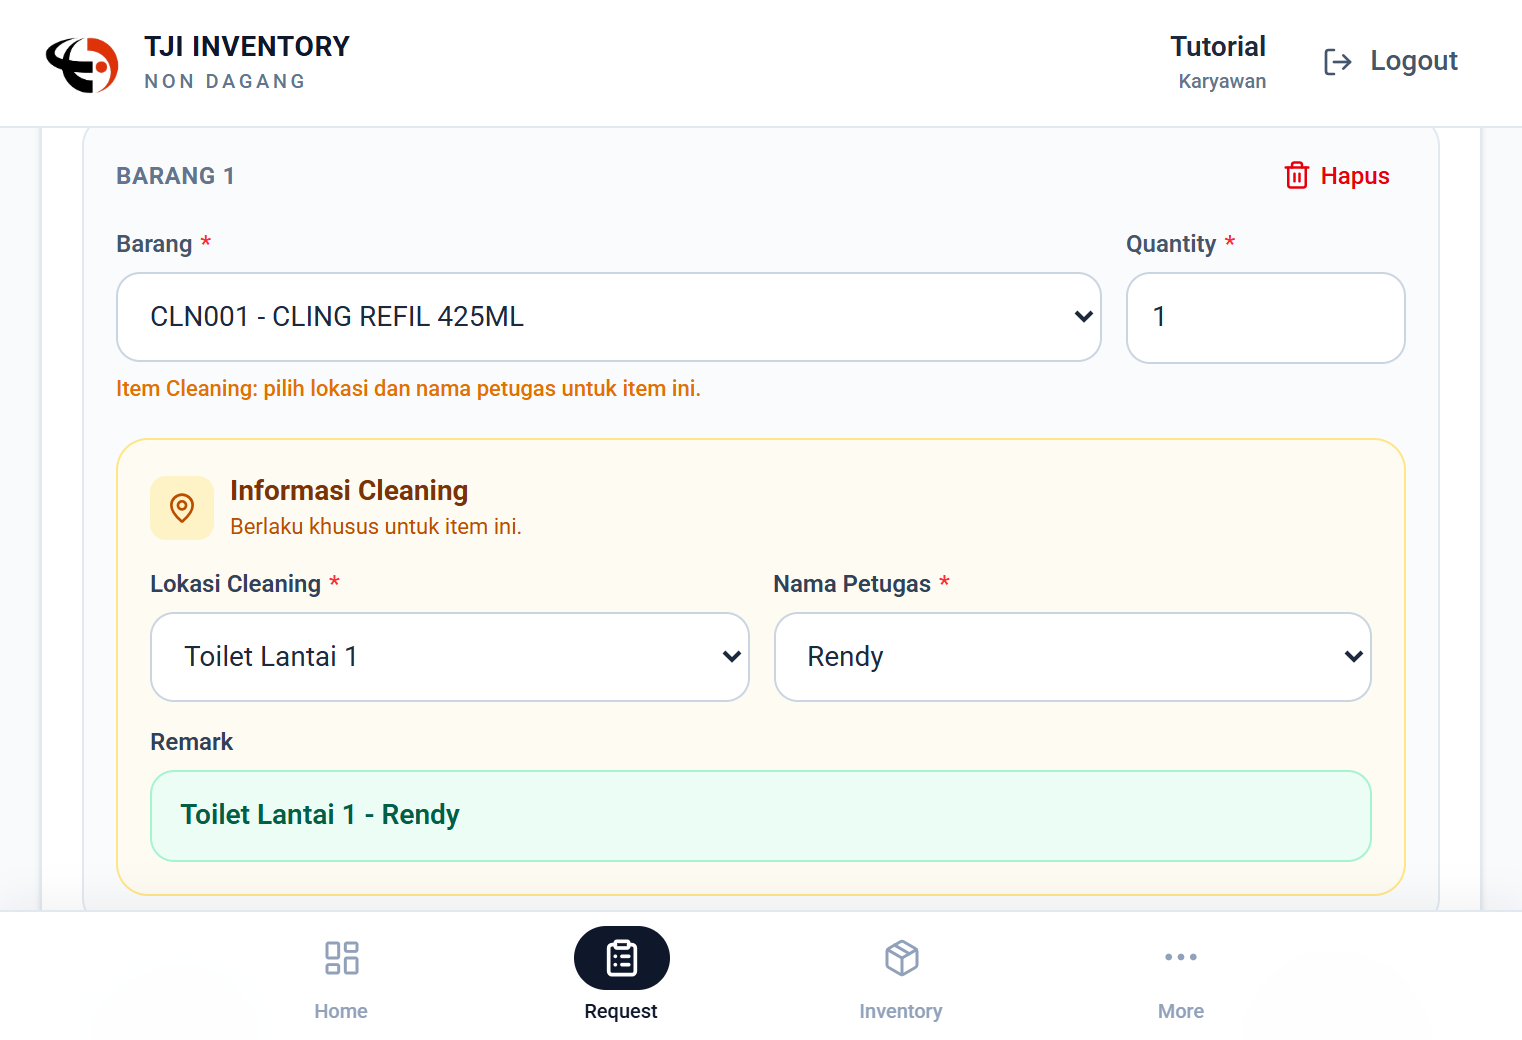
\includegraphics[
						width=0.8\linewidth,
						keepaspectratio
						]{images/Request/Request8.png}
					}
					\only<8>{
						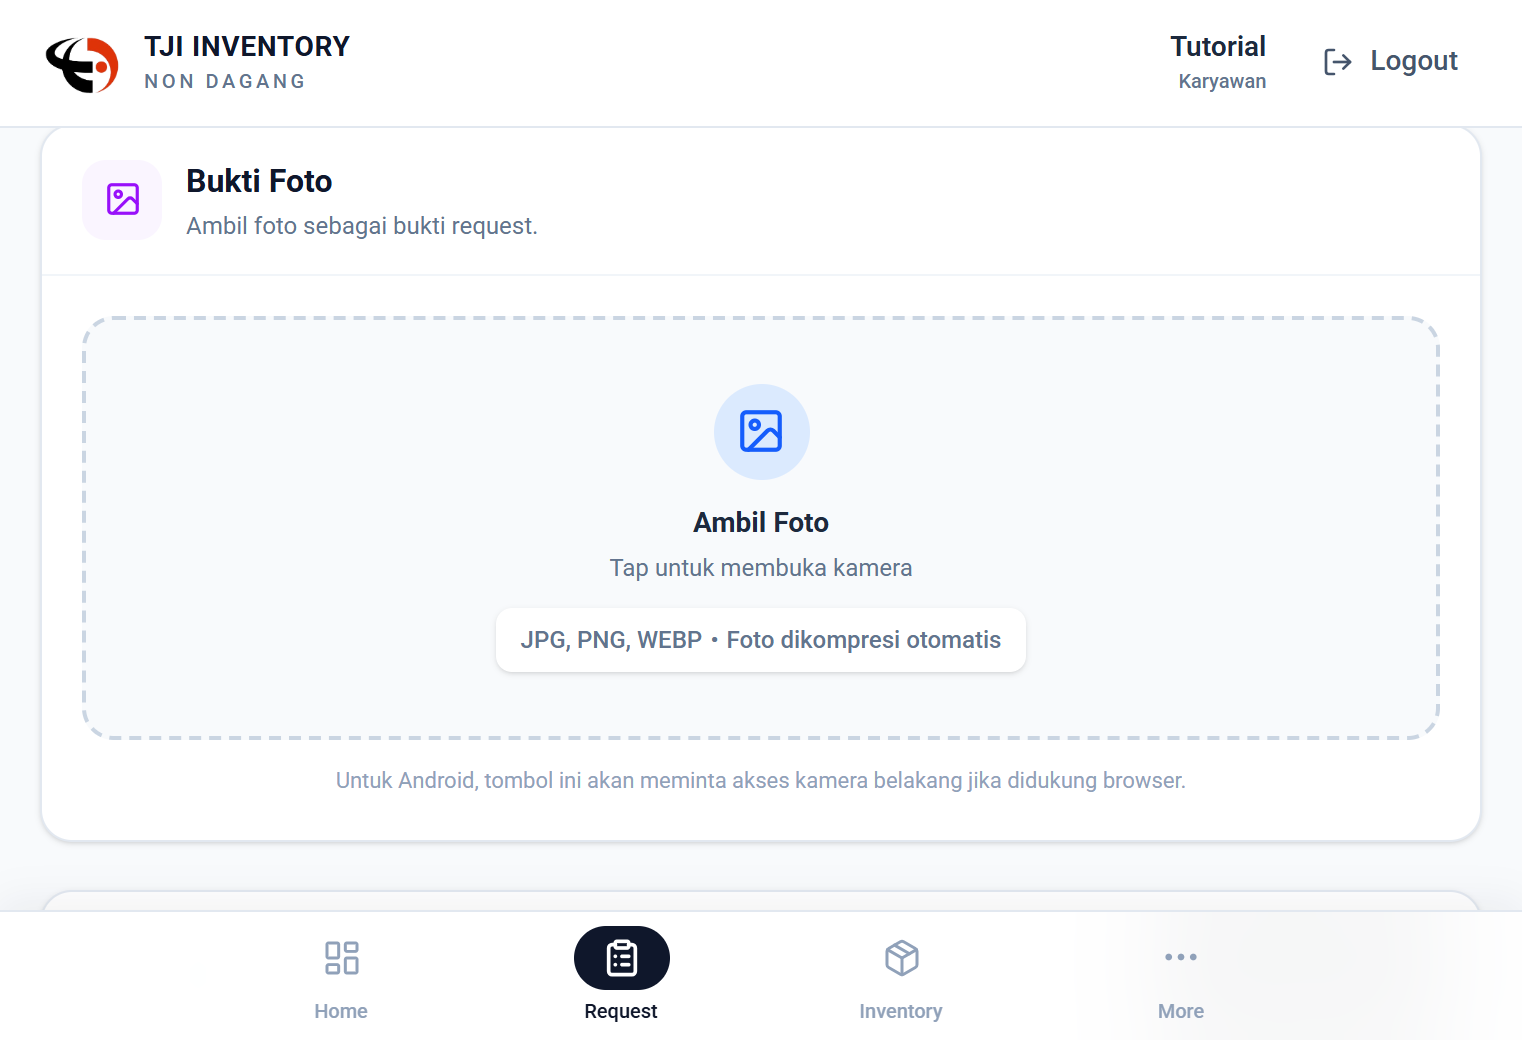
\includegraphics[
						width=0.8\linewidth,
						keepaspectratio
						]{images/Request/Request9.png}
					}
					\only<9>{
						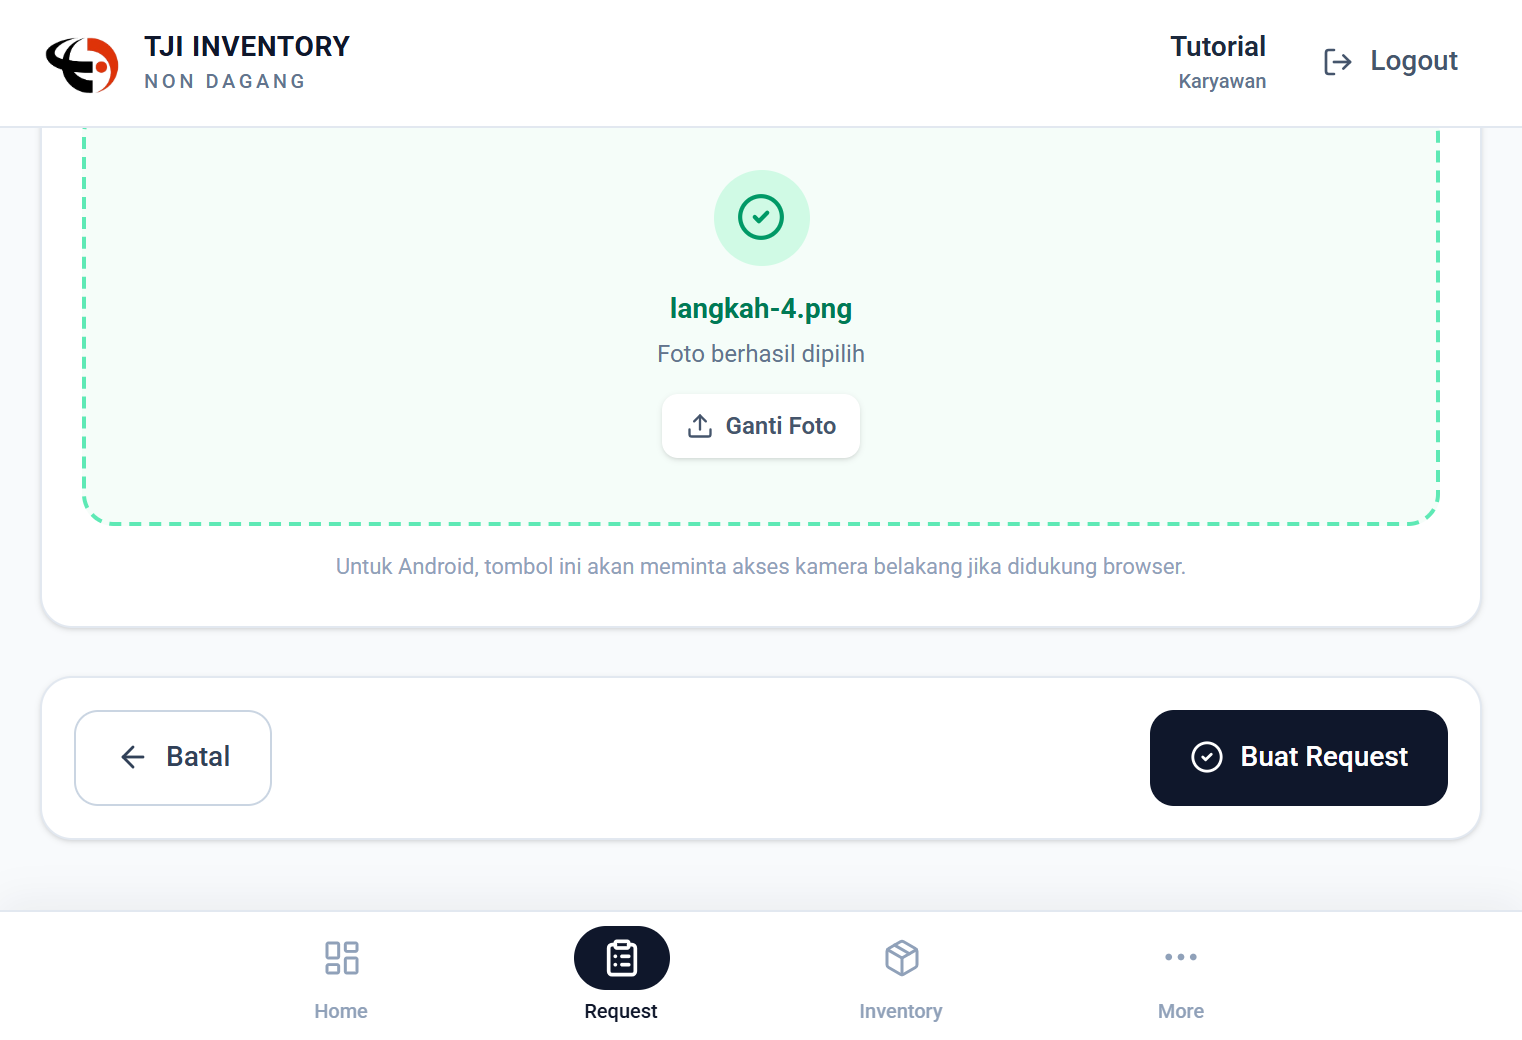
\includegraphics[
						width=0.8\linewidth,
						keepaspectratio
						]{images/Request/Request10.png}
					}
					\only<10>{
						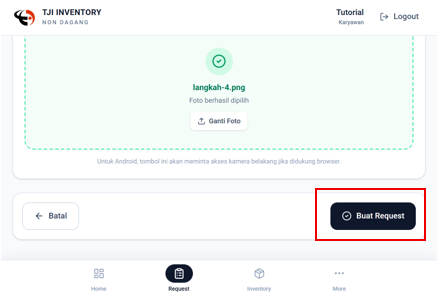
\includegraphics[
						width=0.8\linewidth,
						keepaspectratio
						]{images/Request/Request11.png}
						}				
				};

				% =========================================================
				% HIGHLIGHT
				% =========================================================
				
				\highlight{1}{1.25cm}{2.55cm}{4.0cm}{0.65cm}
				
				\highlight{2}{1.25cm}{1.85cm}{4.0cm}{0.65cm}
				
				\highlight{3}{2.0cm}{0.75cm}{2.7cm}{0.65cm}
				
				\successhighlight{4-10}{0.2cm}{0.2cm}{6.0cm}{3.5cm}
				
			\end{tikzpicture}
			
		\end{center}
		
		
		% =========================================================
		% GAP
		% =========================================================
		
		\column{0.025\textwidth}
		
		
		% =========================================================
		% INSTRUCTION
		% =========================================================
		
		\column{0.325\textwidth}
		
		\vspace{0.02cm}
		
		\sectionlabel{Langkah}
		
		\vspace{0.10cm}
		
		% ---------------------------------------------------------
		% STEP 1
		% ---------------------------------------------------------
		
		\stepcounterdisplay{1}{10}
		
		\stepitem{1}{1}{
			Pilih menu \textbf{Request}.
		}
		
		\vspace{\TutorialGap}
		
		% ---------------------------------------------------------
		% STEP 2
		% ---------------------------------------------------------
		
		\stepcounterdisplay{2}{10}
		
		\stepitem{2}{2}{
			Pilih \textbf{Tambah Permintaan}.
		}
		
		\vspace{\TutorialGap}
		
		% ---------------------------------------------------------
		% STEP 3
		% ---------------------------------------------------------
		
		\stepcounterdisplay{3}{10}
		
		\stepitem{3}{3}{
			Isi \textbf{Nama Requester} dengan nama Anda
			sebagai pemohon, serta isi \textbf{Tujuan Request}.
		}
		
		\vspace{\TutorialGap}
		
		% ---------------------------------------------------------
		% STEP 4
		% ---------------------------------------------------------
		
		\stepcounterdisplay{4}{10}
		
		\stepitem{4}{4}{
			Pilih \textbf{item} yang diperlukan serta isi QTY yang diperlukan.
		}
		
		\vspace{\TutorialGap}
		
		% ---------------------------------------------------------
		% STEP 5
		% ---------------------------------------------------------
		
		\stepcounterdisplay{5}{10}
		
		\stepitem{5}{5}{
			Isi keterangan dengan tujuan penggunaan barang.
		}
		
		
		\vspace{\TutorialGap}
		
		% ---------------------------------------------------------
		% STEP 6
		% ---------------------------------------------------------
		
		\stepcounterdisplay{6}{10}
		
		\stepitem{6}{6}{
			Jika ingin menambahkan item, klik $(+)$ Tambah Barang
		}
		
		\vspace{\TutorialGap}
		
		% ---------------------------------------------------------
		% STEP 7
		% ---------------------------------------------------------
		
		\stepcounterdisplay{7}{10}
		
		\stepitem{7}{7}{
			\textcolor{red}{*} Khusus item barang cleaning keterangan wajib diisi dengan Lokasi Cleaning dan Nama Petugas.
		}
		
		\vspace{\TutorialGap}
		
		% ---------------------------------------------------------
		% STEP 8
		% ---------------------------------------------------------
		
		\stepcounterdisplay{8}{10}
		\stepitem{8}{8}{
			Unggah bukti foto yang menunjukkan kondisi
			atau urgensi penggunaan barang. 
		}
		
		\vspace{\TutorialGap}
		
		% ---------------------------------------------------------
		% STEP 9
		% ---------------------------------------------------------
		
		\stepcounterdisplay{9}{10}
		
		\stepitem{9}{9}{
			Periksa kembali daftar barang sebelum dikirim.
		}
		
		\vspace{\TutorialGap}
		
		% ---------------------------------------------------------
		% STEP 10
		% ---------------------------------------------------------
		
		\stepcounterdisplay{10}{10}
		
		\stepitem{10}{10}{
			Klik \textbf{Buat Request} untuk mengirim permohonan.
		}
		
	\end{columns}
	
\end{frame}
% =========================================================
% TEMPLATE TUTORIAL
% =========================================================

\begin{frame}{03.1 --- Setelah Melakukan Request}
	
	\vspace{-0.25cm}
	
	\begin{columns}[T,totalwidth=\textwidth]
		
		% =========================================================
		% SCREENSHOT
		% =========================================================
		
		\column{0.65\textwidth}
		
		\begin{center}
			
			\begin{tikzpicture}
				
				\node[
				inner sep=0,
				outer sep=0
				] (screen)
				{
					% -----------------------------------------------------
					% SCREENSHOT OVERLAY
					% -----------------------------------------------------
					
					\only<1>{
						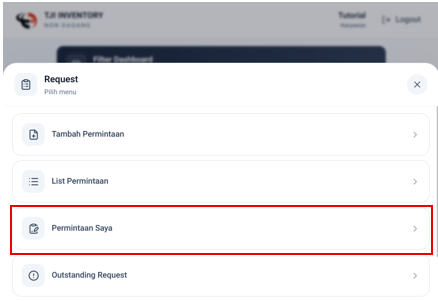
\includegraphics[
						width=0.8\linewidth,
						keepaspectratio
						]{images/PostRequest/Request10.png}
					}
					
					\only<2>{
						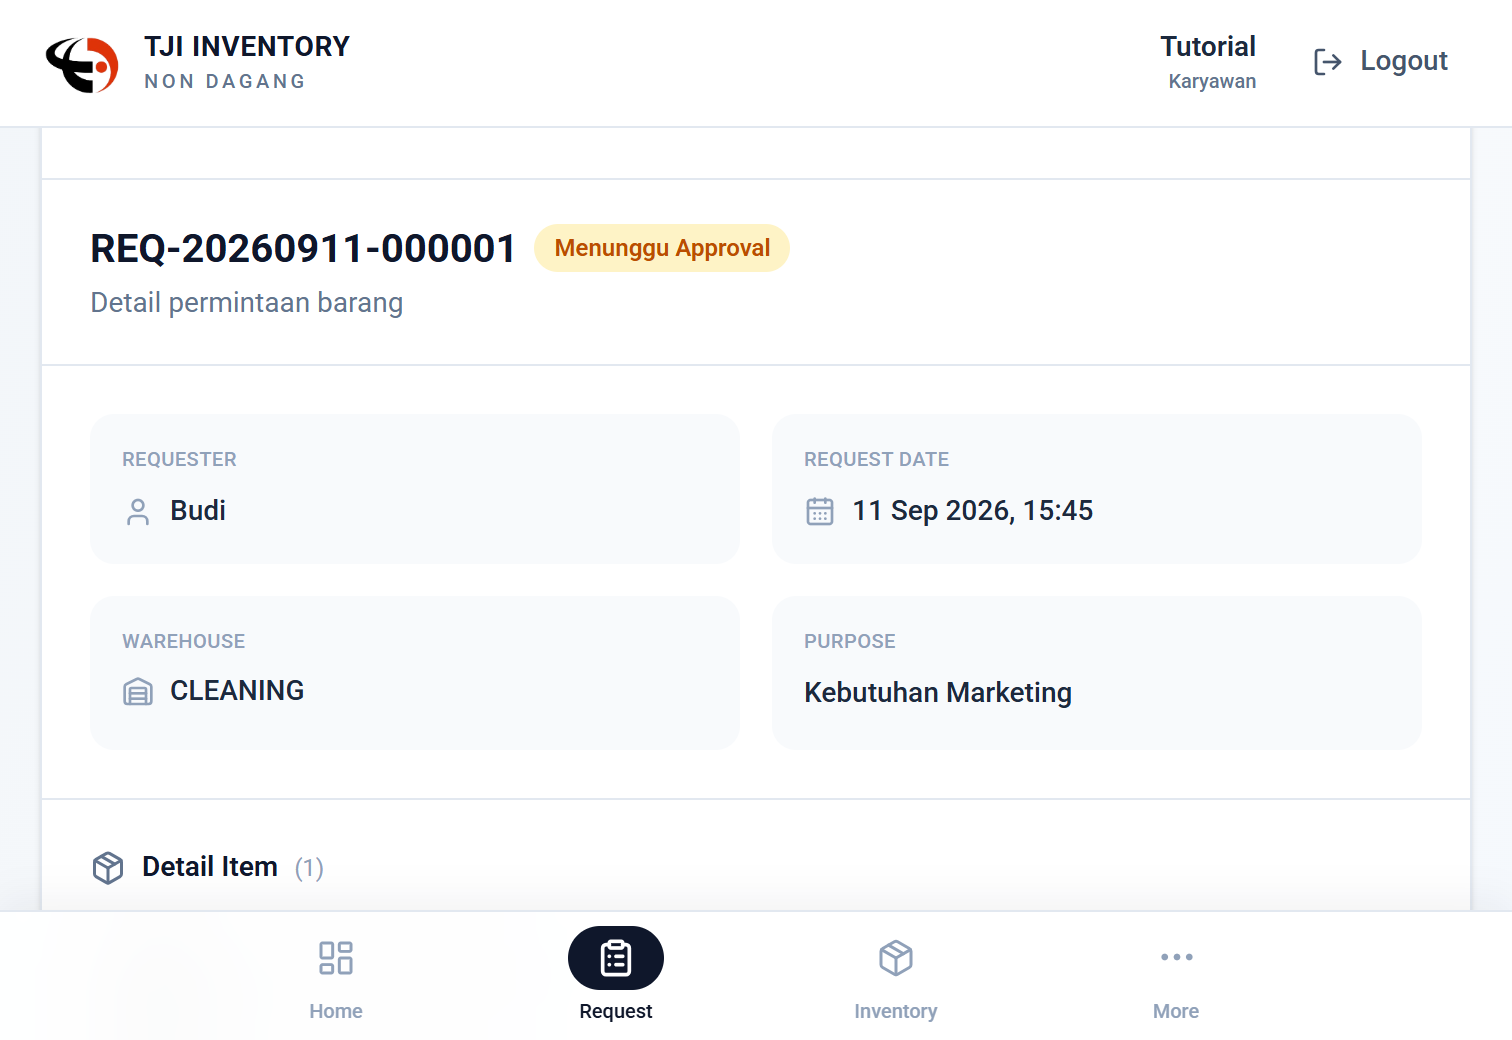
\includegraphics[
						width=0.8\linewidth,
						keepaspectratio
						]{images/PostRequest/Request11.png}
					}
					
					\only<3>{
						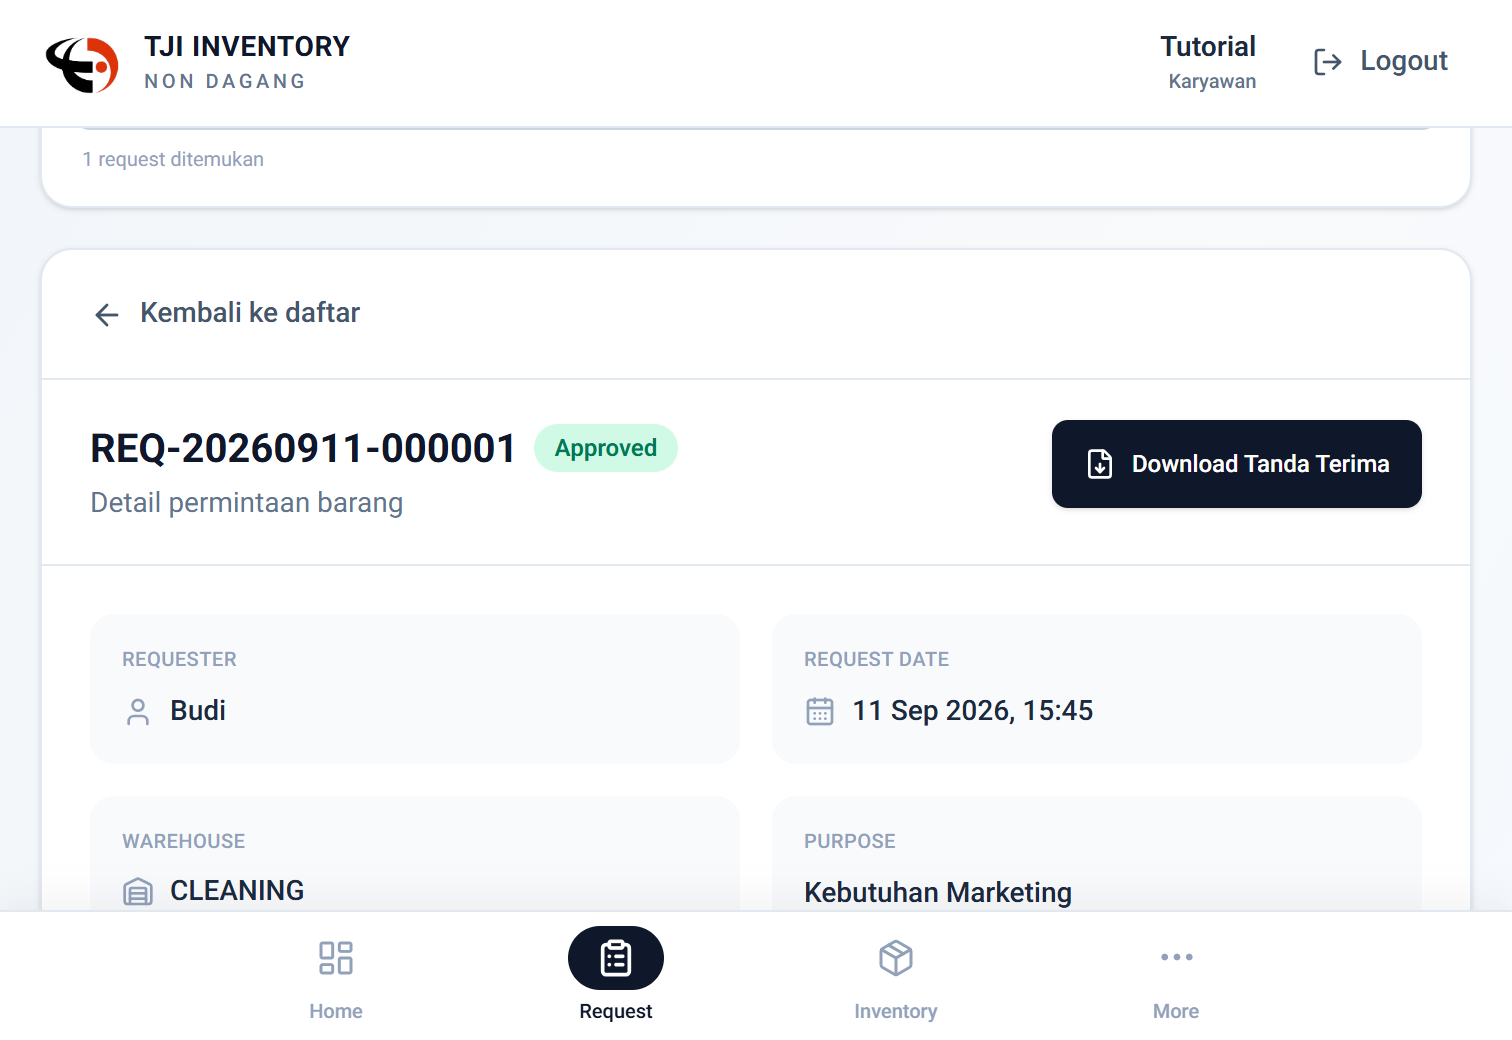
\includegraphics[
						width=0.8\linewidth,
						keepaspectratio
						]{images/PostRequest/Request12.png}
					}
					
					\only<4-5>{
						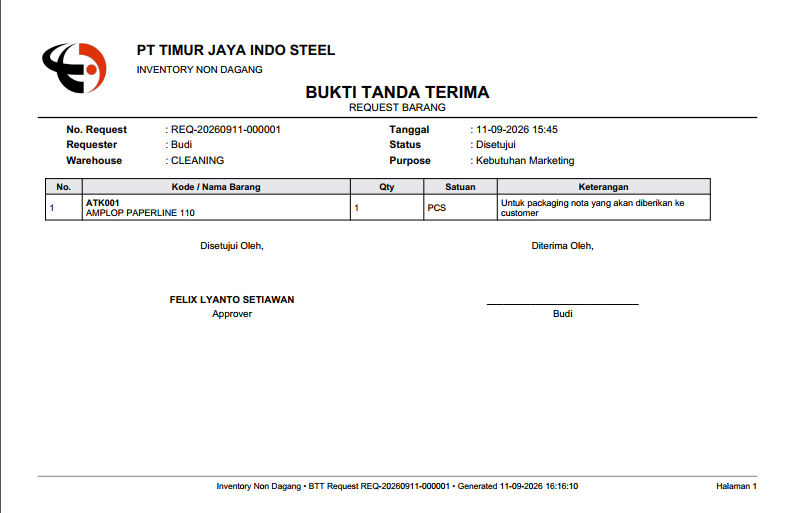
\includegraphics[
						width=0.8\linewidth,
						keepaspectratio
						]{images/PostRequest/Request13.png}
					}
				};
				
				% =========================================================
				% HIGHLIGHT
				% =========================================================
				
				\highlight{1}{Xcm}{Ycm}{Widthcm}{Heightcm}
				
				\highlight{2}{Xcm}{Ycm}{Widthcm}{Heightcm}
				
				\highlight{3}{Xcm}{Ycm}{Widthcm}{Heightcm}
				
				\successhighlight{4-5}{Xcm}{Ycm}{Widthcm}{Heightcm}
				
			\end{tikzpicture}
			
		\end{center}
		
		
		% =========================================================
		% GAP
		% =========================================================
		
		\column{0.025\textwidth}
		
		
		% =========================================================
		% LANGKAH
		% =========================================================
		
		\column{0.325\textwidth}
		
		\vspace{0.02cm}
		
		\sectionlabel{Langkah}
		
		\vspace{0.10cm}
		
		% STEP 1
		\stepcounterdisplay{1}{5}
		
		\stepitem{1}{1}{
			Pilih Request $>$ Permintaan Saya
		}
		
		\vspace{\TutorialGap}
		
		% STEP 2
		\stepcounterdisplay{2}{5}
		
		\stepitem{2}{2}{
    Perhatikan status permohonan. Status \textbf{Menunggu Approval}
    berarti permintaan sedang diproses oleh petugas. Jika status berubah
    menjadi \textbf{Approved}, berarti permohonan telah disetujui.
		}
		
		\vspace{\TutorialGap}
		
		% STEP 3
		\stepcounterdisplay{3}{5}
		
		\stepitem{3}{3}{
			Pilih Download Tanda Terima.
		}
		
		\vspace{\TutorialGap}
		
		% STEP 4
		\stepcounterdisplay{4}{5}
		
		\stepitem{4}{4}{
		Print Tanda Terima format kertas PRS.
		}
		
		\vspace{\TutorialGap}
		
		% STEP 5
		\stepcounterdisplay{5}{5}
		
		\stepitem{5}{5}{
			Saat menerima barang, tandatangani tanda terima pada bagian \textbf{Diterima Oleh}, kemudian serahkan tanda terima tersebut
			kepada petugas.
		}
	\end{columns}
	
\end{frame}
\begin{frame}{Attention}
	
	\vfill
	
	\begin{center}
		
		\begin{minipage}{0.90\textwidth}
			
			\warningbox{Perlu Diperhatikan}{
				\large
				\begin{itemize}
					\item Satu request hanya dapat berisi barang dari satu kategori.\\
					Contoh: barang Cleaning dan ATK tidak dapat digabungkan dalam satu request.
					
					\vspace{0.25cm}
					
					\item Pada perangkat Android, iOS, dan Tablet, bukti foto dapat diunggah langsung menggunakan kamera perangkat. Pada versi Desktop, bukti foto dapat diunggah dalam format JPG, PNG, atau WEBP.
				\end{itemize}
			}
			
		\end{minipage}
		
	\end{center}
	
	\vfill
	
\end{frame}


% =========================================================
% AKTIVASI IZIN KAMERA CHROME ANDROID
% =========================================================

\begin{frame}{Aktivasi Izin Kamera --- Chrome Android}
	
	\vspace{-0.15cm}
	
	\begin{center}
		
		\begin{minipage}{0.92\textwidth}
			
			\warningbox{Attention}{
				\large
				Kamera diperlukan untuk mengambil atau mengunggah
				\textbf{bukti foto} pada proses request.
				
				\vspace{0.15cm}
				
				Jika kamera tidak dapat digunakan, pastikan izin kamera
				untuk Chrome pada perangkat Android telah diaktifkan.
			}
			
			\vspace{0.30cm}
			
			\textbf{\Large Cara Mengaktifkan Izin Kamera}
			
			\vspace{0.15cm}
			
			\begin{enumerate}
				\item Buka \textbf{Pengaturan Android}
				$\rightarrow$ \textbf{Aplikasi}
				$\rightarrow$ \textbf{Chrome}
				$\rightarrow$ \textbf{Izin}.
				
				\vspace{0.18cm}
				
				\item Pilih \textbf{Kamera}, kemudian ubah izin menjadi
				\textbf{Izinkan} atau \textbf{Izinkan hanya saat aplikasi digunakan}.
			\end{enumerate}
			
			\vspace{0.15cm}
			
			\successbox{Setelah Diaktifkan}{
				Kembali ke Chrome dan buka kembali halaman aplikasi
				TJI Inventory Non-Dagang untuk mencoba mengambil foto.
			}
			
		\end{minipage}
		
	\end{center}
	
	\vfill
	
\end{frame}




% =========================================================
% APPROVAL
% =========================================================


% =========================================================

% =========================================================
% APPROVAL
% =========================================================

\begin{frame}{03.2 --- Approval}
	
	\vspace{-0.25cm}
	
	\begin{columns}[T,totalwidth=\textwidth]
		
		% =========================================================
		% SCREENSHOT
		% =========================================================
		
		\column{0.65\textwidth}
		
		\begin{center}
			
			\begin{tikzpicture}
				
				\node[
				inner sep=0,
				outer sep=0
				] (screen)
				{
					\only<1>{
						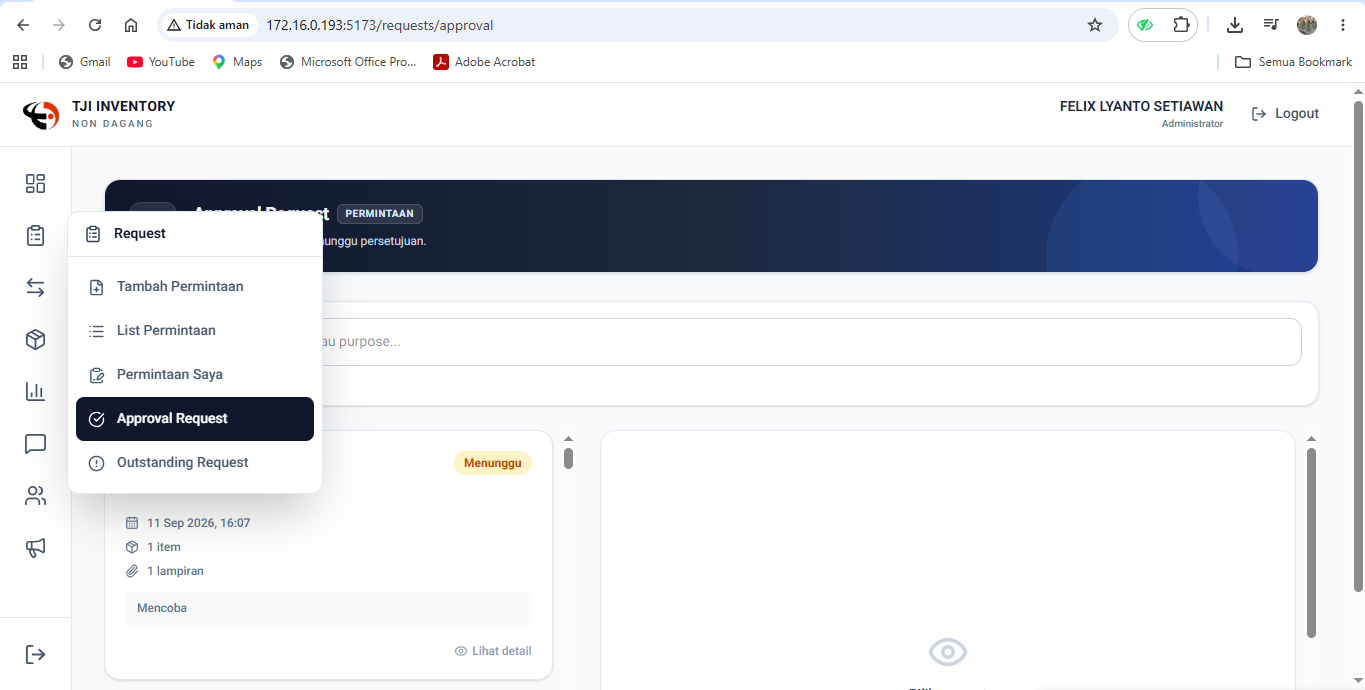
\includegraphics[
						width=\linewidth,
						keepaspectratio
						]{images/Approval/Approval1.png}
					}
					
					\only<2>{
						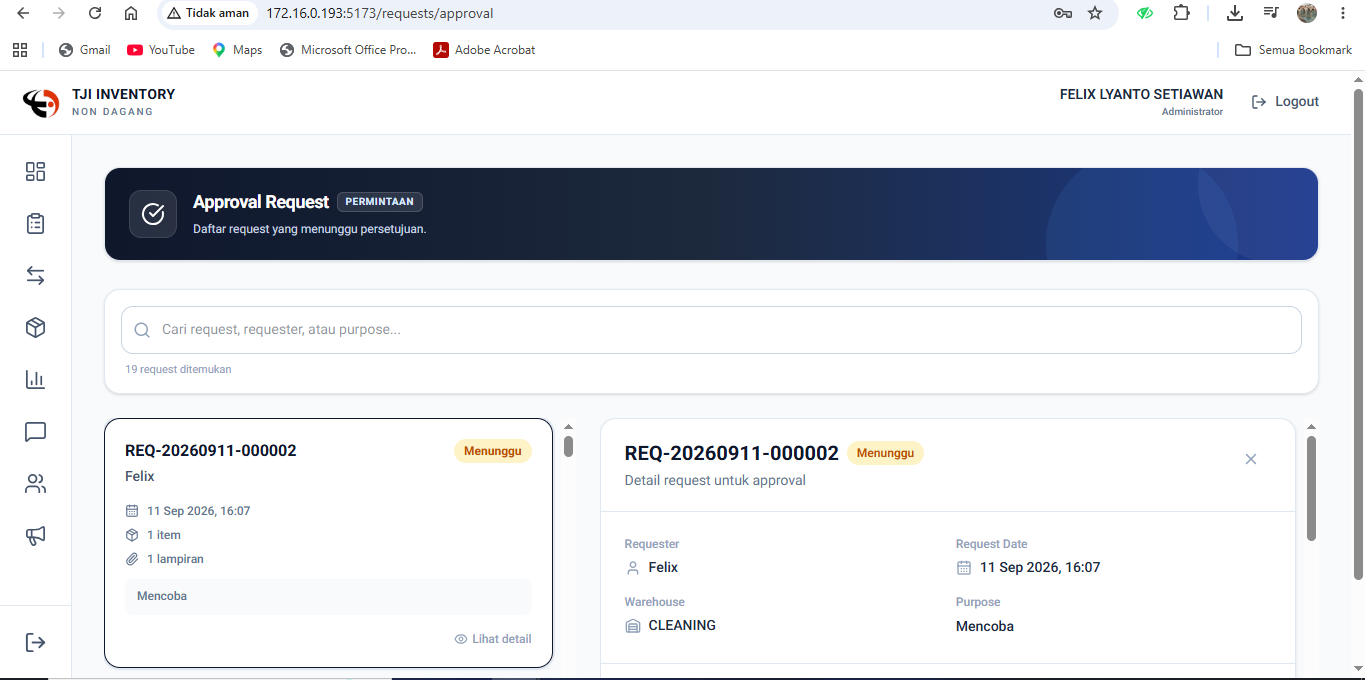
\includegraphics[
						width=\linewidth,
						keepaspectratio
						]{images/Approval/Approval2.png}
					}
					
					\only<3>{
						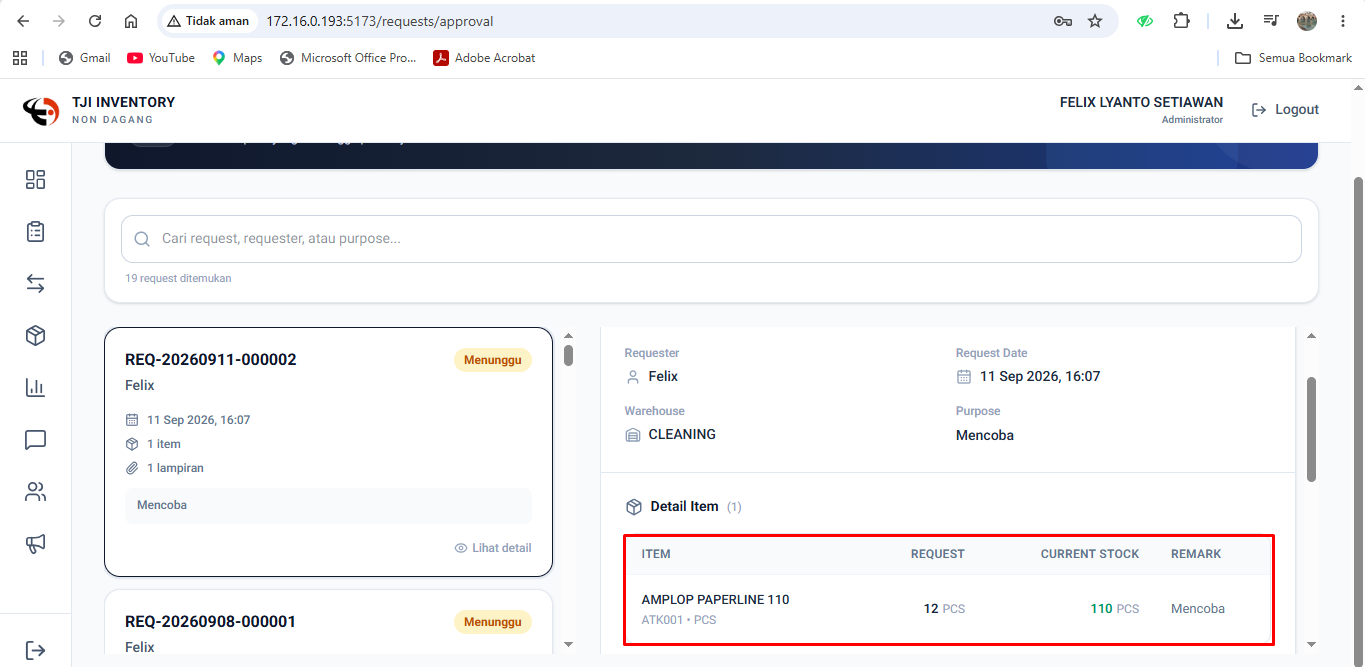
\includegraphics[
						width=\linewidth,
						keepaspectratio
						]{images/Approval/Approval3.png}
					}
					
					\only<4>{
						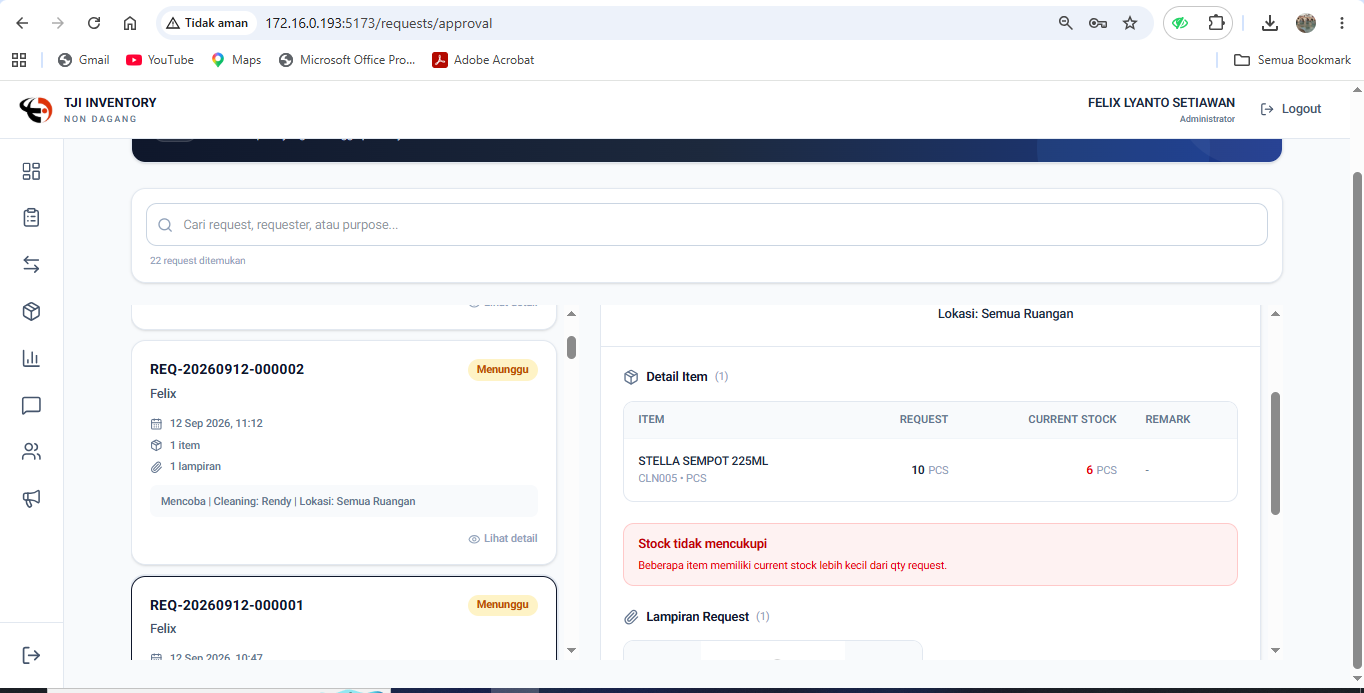
\includegraphics[
						width=\linewidth,
						keepaspectratio
						]{images/Approval/Approval4.png}
					}
					
					\only<5>{
						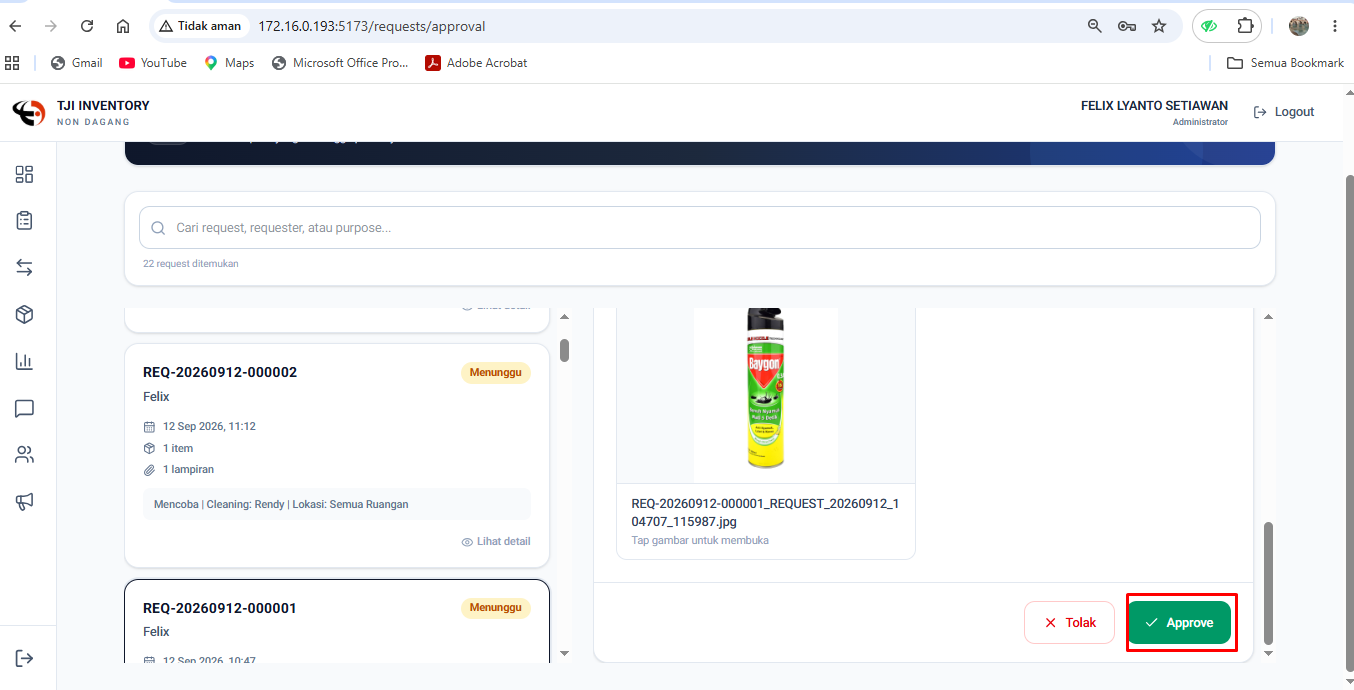
\includegraphics[
						width=\linewidth,
						keepaspectratio
						]{images/Approval/Approval5.png}
					}
					
					\only<6>{
						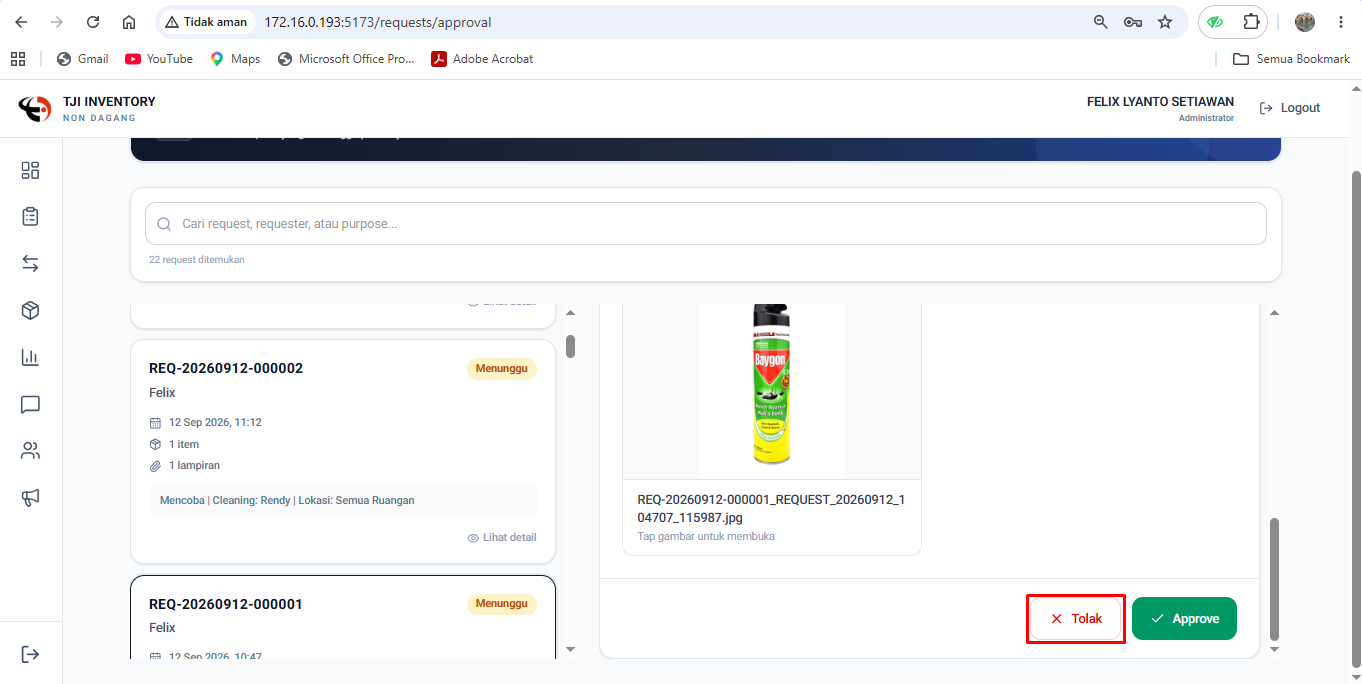
\includegraphics[
						width=0.95\linewidth,
						keepaspectratio
						]{images/Approval/Approval6.png}
					}
					
					\only<7>{
						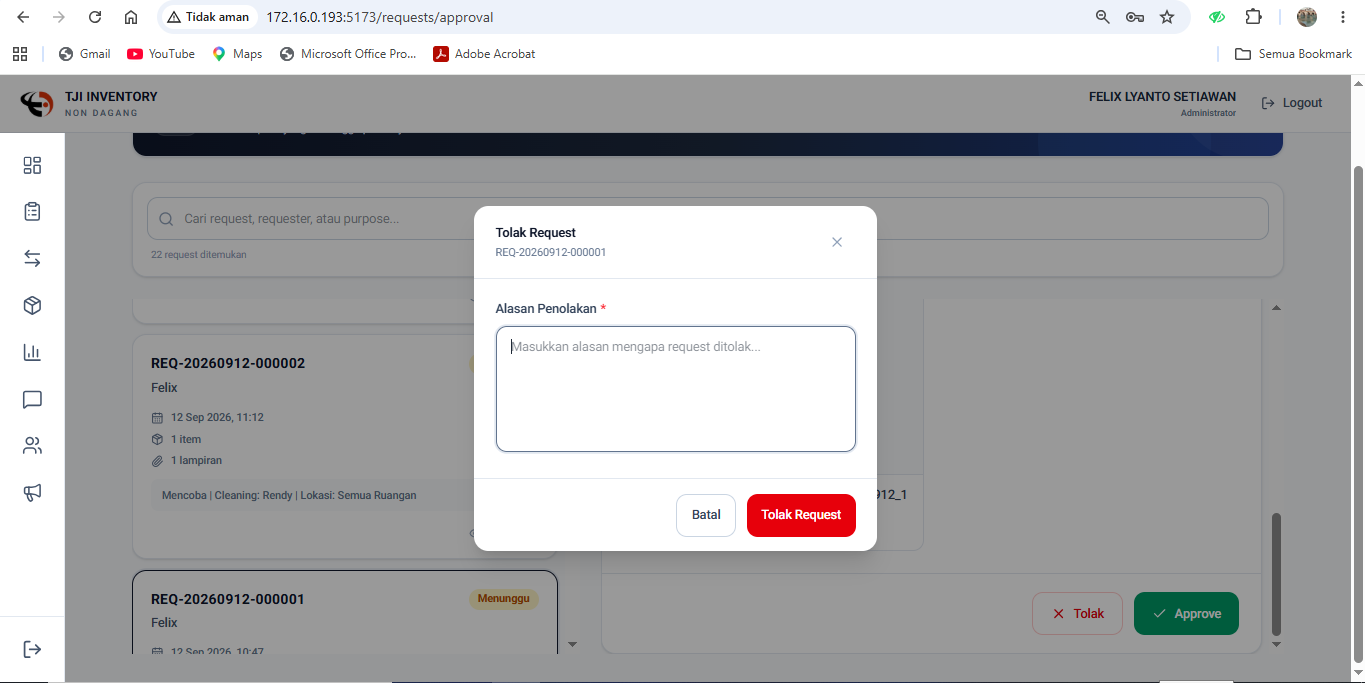
\includegraphics[
						width=0.95\linewidth,
						keepaspectratio
						]{images/Approval/Approval7.png}
					}
					
					\only<8>{
						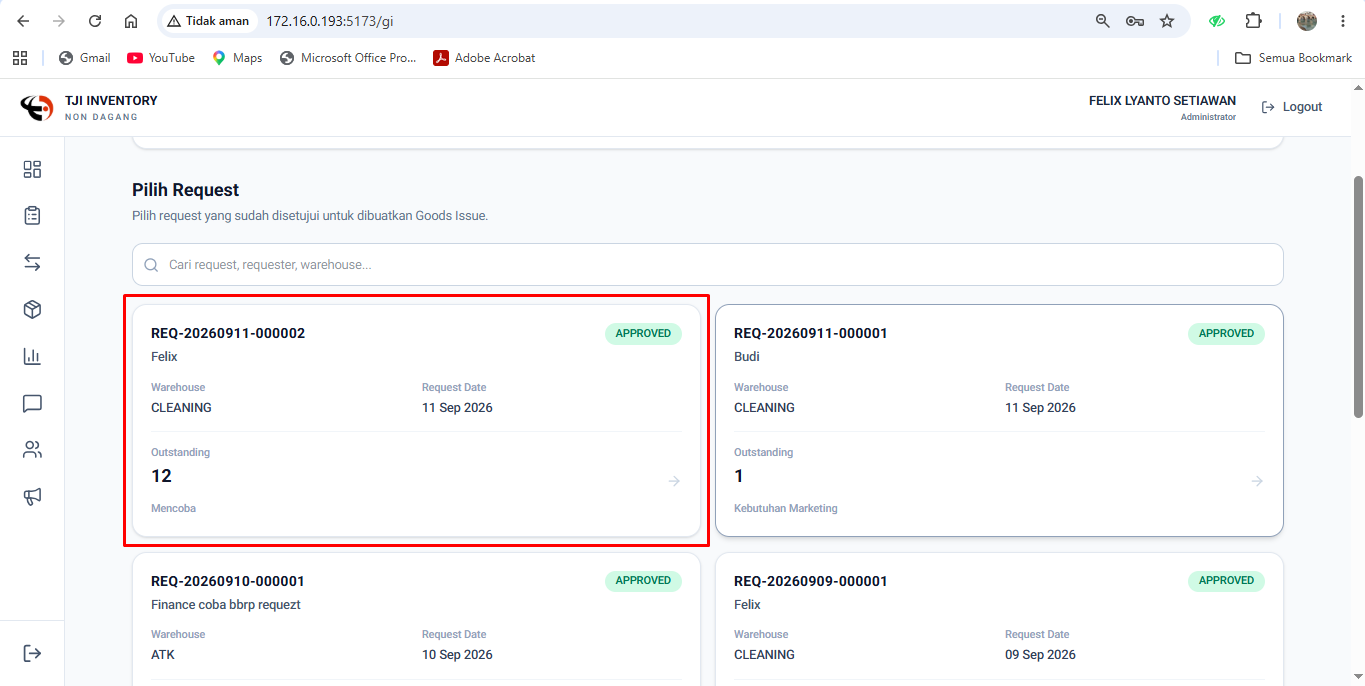
\includegraphics[
						width=0.95\linewidth,
						keepaspectratio
						]{images/Approval/Approval8.png}
					}
				};
				
			\end{tikzpicture}
			
		\end{center}
		
		
		% =========================================================
		% GAP
		% =========================================================
		
		\column{0.025\textwidth}
		
		
		% =========================================================
		% LANGKAH
		% =========================================================
		
		\column{0.325\textwidth}
		
		\vspace{0.02cm}
		
		\sectionlabel{Langkah}
		
		\vspace{0.10cm}
		
		
		% =========================================================
		% STEP 1
		% =========================================================
		
		\stepcounterdisplay{1}{8}
		
		\stepitem{1}{1}{
			Pilih \textbf{Approval Request}.
		}
		
		\vspace{\TutorialGap}
		
		
		% =========================================================
		% STEP 2
		% =========================================================
		
		\stepcounterdisplay{2}{8}
		
		\stepitem{2}{2}{
			Pilih data request yang akan dilakukan persetujuan.
		}
		
		\vspace{\TutorialGap}
		
		
		% =========================================================
		% STEP 3
		% =========================================================
		
		\stepcounterdisplay{3}{8}
		
		\stepitem{3}{3}{
			Periksa quantity yang diminta dan pastikan stok mencukupi.
		}
		
		\vspace{\TutorialGap}
		
		
		% =========================================================
		% STEP 4
		% =========================================================
		
		\stepcounterdisplay{4}{8}
		
		\stepitem{4}{4}{
			Jika quantity request melebihi ketersediaan stok,
			akan muncul notifikasi seperti berikut.
		}
		
		\vspace{\TutorialGap}
		
		
		% =========================================================
		% STEP 5
		% =========================================================
		
		\stepcounterdisplay{5}{8}
		
		\stepitem{5}{5}{
			Jika request sesuai, Pilih \textbf{Approve}.
		}
		
		\vspace{\TutorialGap}
		
		
		% =========================================================
		% STEP 6
		% =========================================================
		
		\stepcounterdisplay{6}{8}
		
		\stepitem{6}{6}{
			Jika request tidak sesuai, Pilih Tolak
		}
		
		\vspace{\TutorialGap}
		
		
		% =========================================================
		% STEP 7
		% =========================================================
		
		\stepcounterdisplay{7}{8}
		
		\stepitem{7}{7}{
			\textcolor{red}{*} Isi Alasan Penolakan (apabila Pilih Tolak)
		}
		
		\vspace{\TutorialGap}
		
		
		% =========================================================
		% STEP 8
		% =========================================================
		
		\stepcounterdisplay{8}{8}
		
		\stepitem{8}{8}{
			Request dapat diproses oleh warehouse.
		}
		
		
		% =========================================================
		% APPROVED BOX
		% =========================================================
		
		\vspace{0.12cm}
		
		\only<5>{
			\successbox{Approved}{
				Request telah disetujui dan dapat diproses
				oleh Transaksi.
			}
		}
		
	\end{columns}
	
\end{frame}


\begin{frame}{Alur Transaksi}
	
	\vspace{-0.05cm}
	
	\sectionlabel{Alur Proses Transaksi}
	
	\vspace{0.40cm}
	
	\begin{center}
		
		
\begin{tikzpicture}[node distance=0.75cm]
			
			% ---------------------------------------------------------
			% STEP 6
			% ---------------------------------------------------------
			
			\node[
			draw=Primary,
			fill=Secondary,
			rounded corners=7pt,
			minimum width=2.8cm,
			minimum height=1.25cm,
			align=center,
			font=\large
			]
			(transaction)
			{\textbf{Pilih Request}};
			
			% ---------------------------------------------------------
			% STEP 7
			% ---------------------------------------------------------
			
			\node[
			draw=Primary,
			fill=Secondary,
			rounded corners=7pt,
			minimum width=2.8cm,
			minimum height=1.25cm,
			align=center,
			font=\large,
			right=of transaction
			]
			(request)
			{\textbf{Buat Goods Issue}};
			
			% ---------------------------------------------------------
			% STEP 8
			% ---------------------------------------------------------
			
			\node[
			draw=Warning,
			fill=WarningLight,
			rounded corners=7pt,
			minimum width=2.8cm,
			minimum height=1.25cm,
			align=center,
			font=\large,
			right=of request
			]
			(gi)
			{\textbf{Posting Goods Issue}};
			
			% ---------------------------------------------------------
			% STEP 9
			% ---------------------------------------------------------
			
			\node[
			draw=Success,
			fill=SuccessLight,
			rounded corners=7pt,
			minimum width=2.8cm,
			minimum height=1.25cm,
			align=center,
			font=\large,
			right=of gi
			]
			(confirm)
			{\textbf{Selesai}};
			
			% ---------------------------------------------------------
			% STEP 10
			% ---------------------------------------------------------
			
			
			% ---------------------------------------------------------
			% ARROWS
			% ---------------------------------------------------------
			
			\draw[->,thick]
			(transaction) -- (request);
			
			\draw[->,thick]
			(request) -- (gi);
			
			\draw[->,thick]
			(gi) -- (confirm);
			
			
		\end{tikzpicture}
		
	\end{center}
	
	\vspace{0.50cm}
	
	% =========================================================
	% STEP 6
	% =========================================================
	
	\only<1>{
		\infobox{STEP 6 --- Pilih Request}{
			Petugas memilih request yang telah berstatus \textbf{APPROVED}
			untuk diproses pada transaksi pengeluaran barang (Buat Goods Issue).
		}
	}
	
	% =========================================================
	% STEP 7
	% =========================================================
	
	\only<2>{
		\infobox{STEP 7 --- Buat Goods Issue}{
		Petugas membuat Goods Issue (Pengeluaran Barang) berdasarkan
		request yang telah dipilih, dan harus melengkapi
		data pengeluaran barang sebelum diproses.
		}
	}
	
	% =========================================================
	% STEP 8
	% =========================================================
	
	\only<3>{
		\infobox{STEP 8 --- Posting Goods Issue}{
			Petugas melakukan posting Goods Issue
			untuk mencatat pengeluaran barang.
		}
	}
	
	% =========================================================
	% STEP 9
	% =========================================================
	
	\only<4>{
		\infobox{STEP 9 --- Selesai}{
			Proses Goods Issue berhasil dilakukan dan transaksi tercatat di sistem, sehingga stok dalam sistem berkurang sesuai dengan barang yang dikeluarkan.
		}
	}
	
	% =========================================================
	% STEP 10
	% =========================================================
	
	\only<5>{
		\infobox{STEP 10 --- Selesai}{
			Stok inventory diperbarui sesuai dengan
			barang dan quantity yang telah dikeluarkan.
		}
	}
	
\end{frame}






% =========================================================
% GOODS ISSUE
% =========================================================

% =========================================================
% GOODS ISSUE
% =========================================================

\begin{frame}{04 --- Goods Issue (Pengeluaran Barang)}
	
	\vspace{-0.25cm}
	
	\begin{columns}[T,totalwidth=\textwidth]
		
		\column{0.65\textwidth}
		
		\begin{center}
			
			\begin{tikzpicture}
				
				\node[
				inner sep=0,
				outer sep=0
				] (screen)
				{
					\only<1>{
						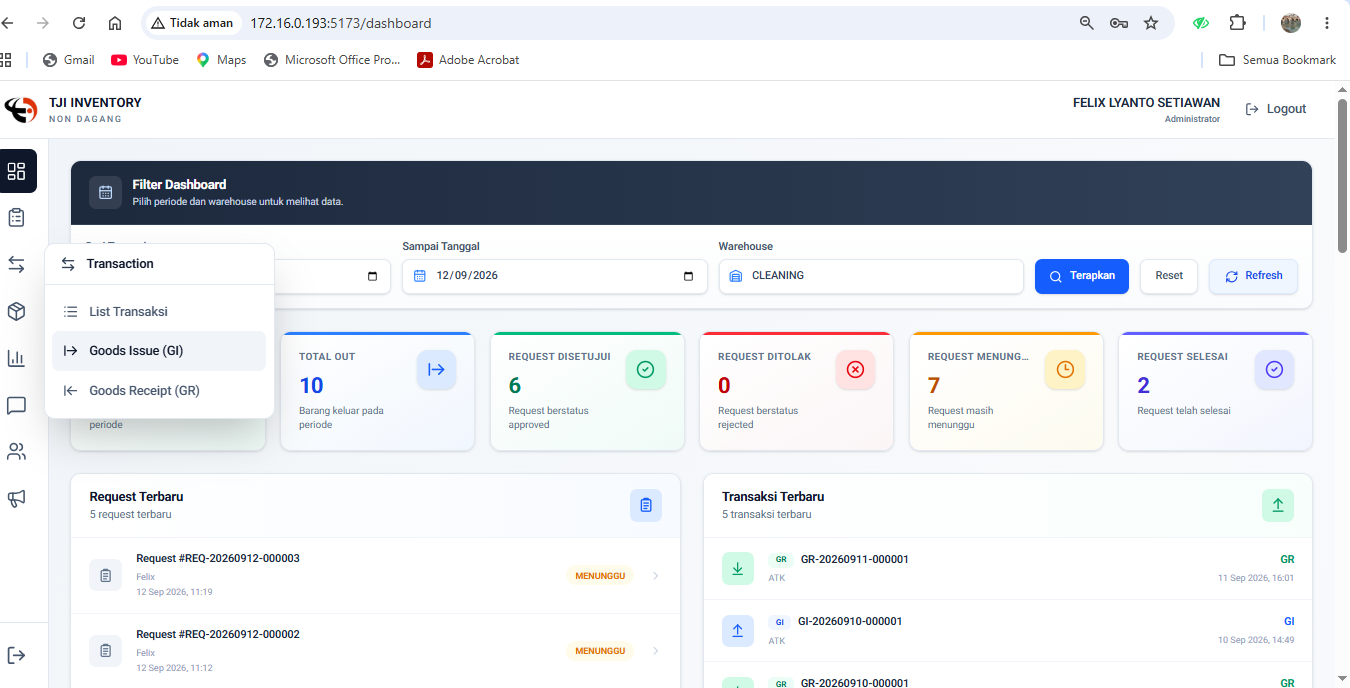
\includegraphics[
						width=0.95\linewidth,
						keepaspectratio
						]{images/GI/GI1.png}
					}
					
					\only<2>{
						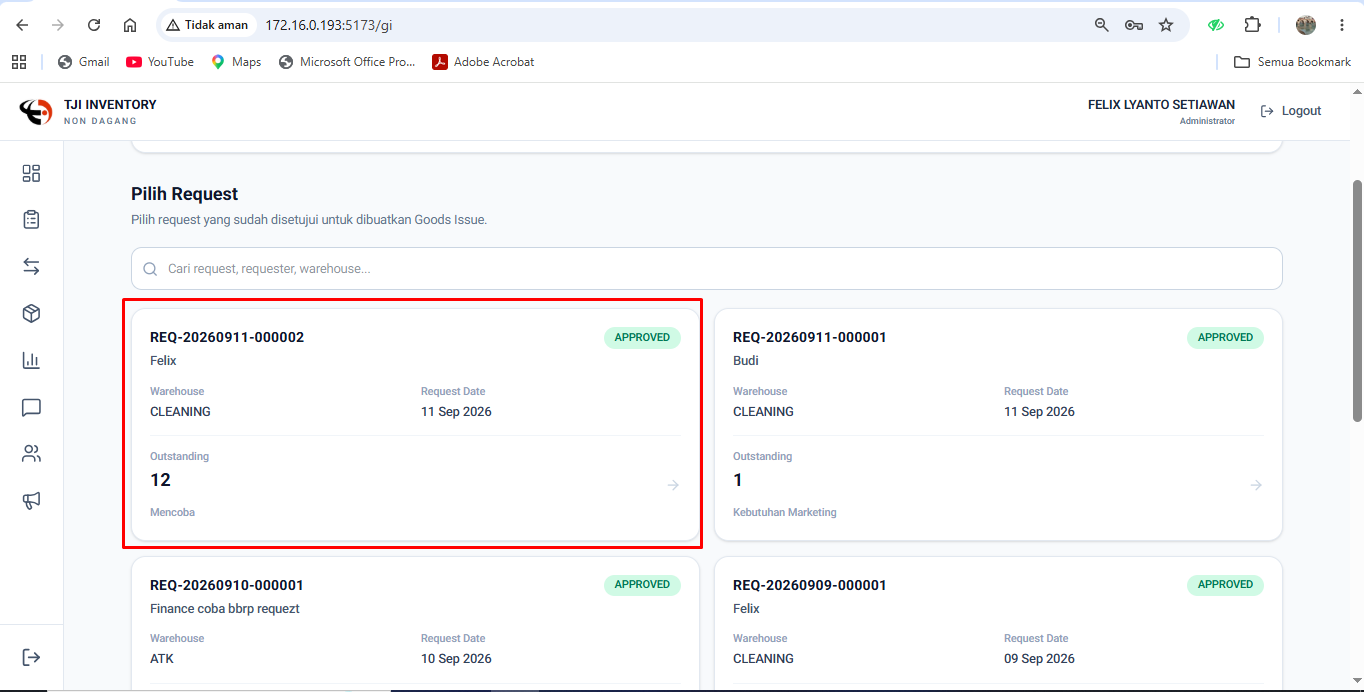
\includegraphics[
						width=0.95\linewidth,
						keepaspectratio
						]{images/GI/GI2.png}
					}
					
					\only<3>{
						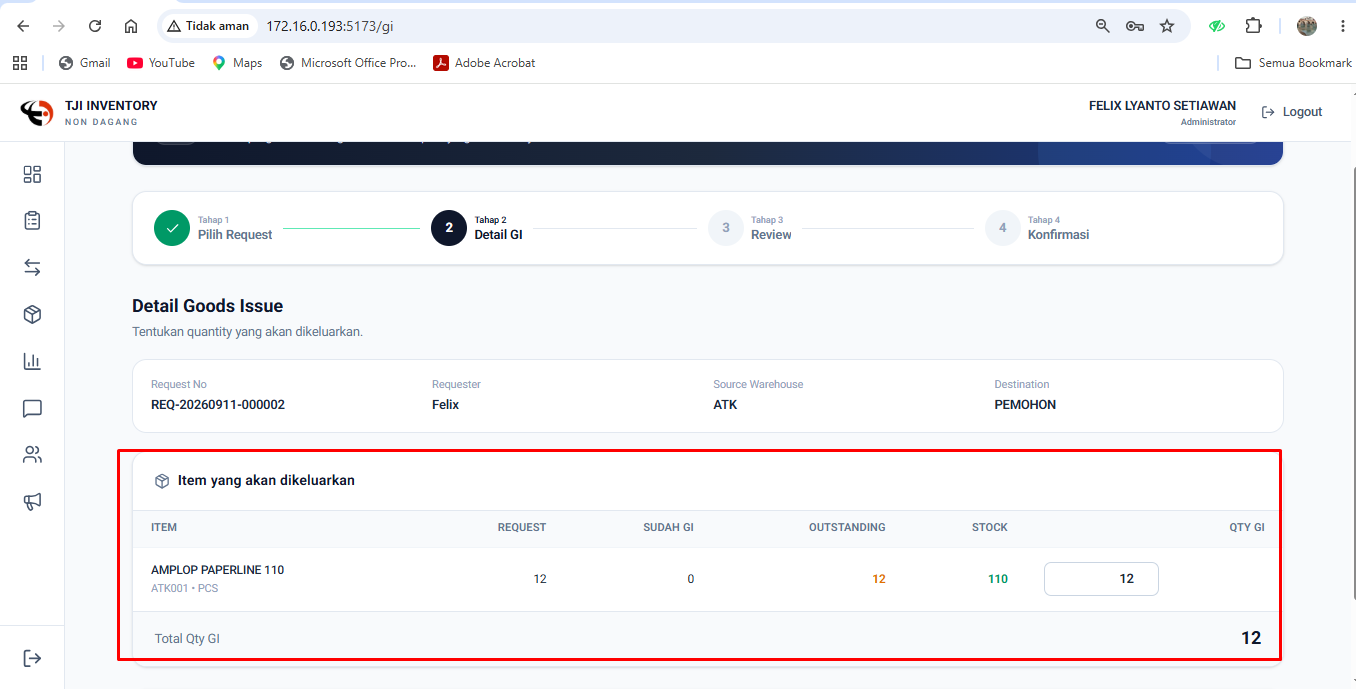
\includegraphics[
						width=0.95\linewidth,
						keepaspectratio
						]{images/GI/GI3.png}
					}
					
					\only<4>{
						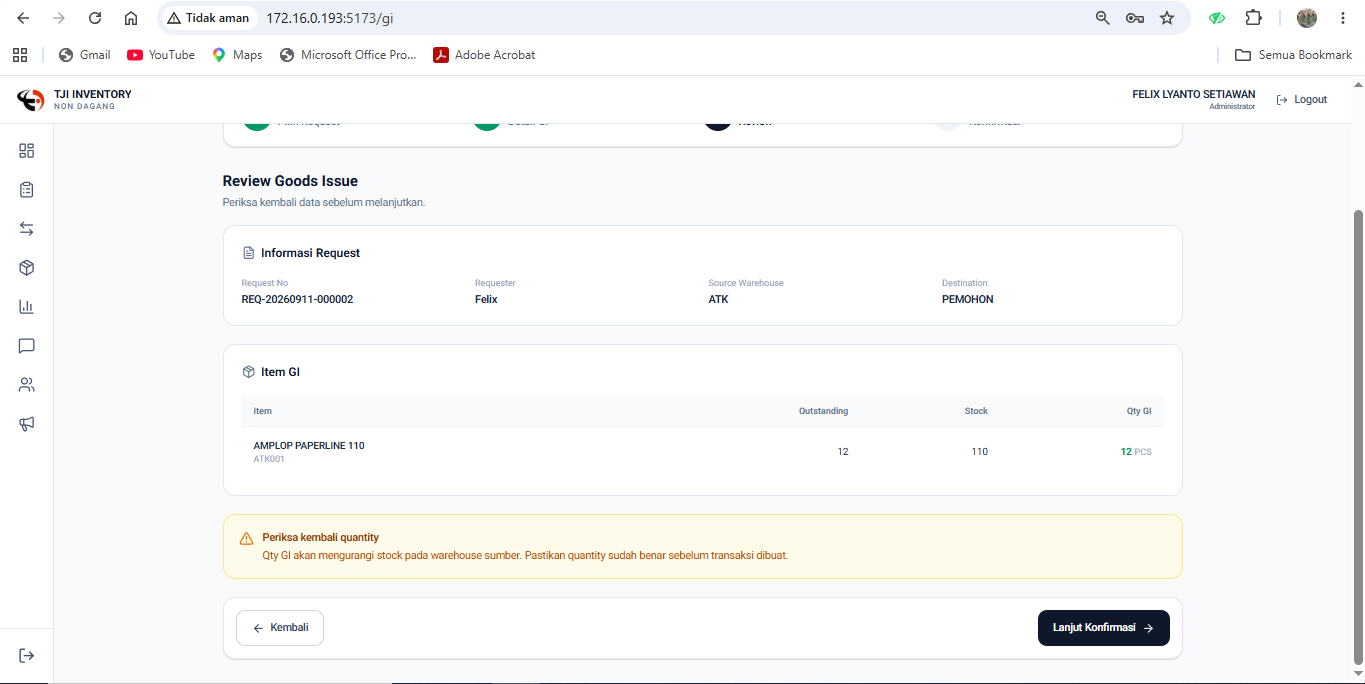
\includegraphics[
						width=0.95\linewidth,
						keepaspectratio
						]{images/GI/GI4.png}
					}
					
					\only<5>{
						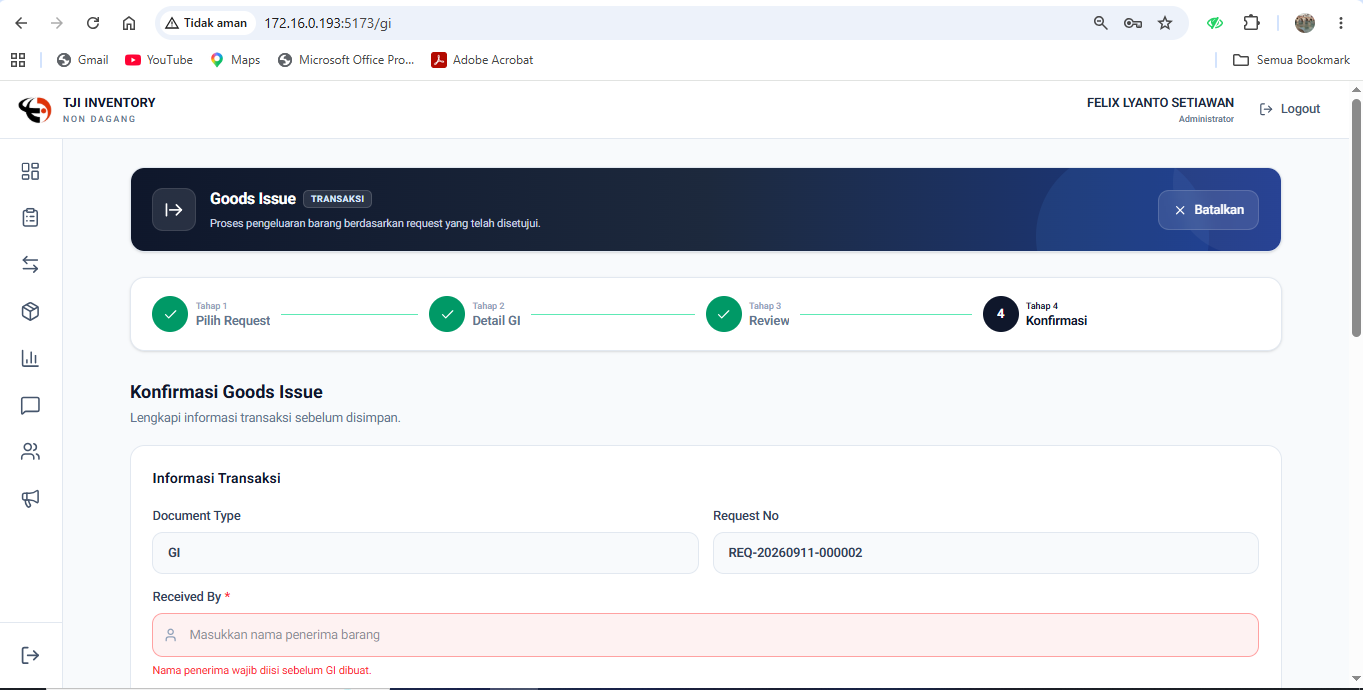
\includegraphics[
						width=0.95\linewidth,
						keepaspectratio
						]{images/GI/GI5.png}
					}
					
					\only<6>{
						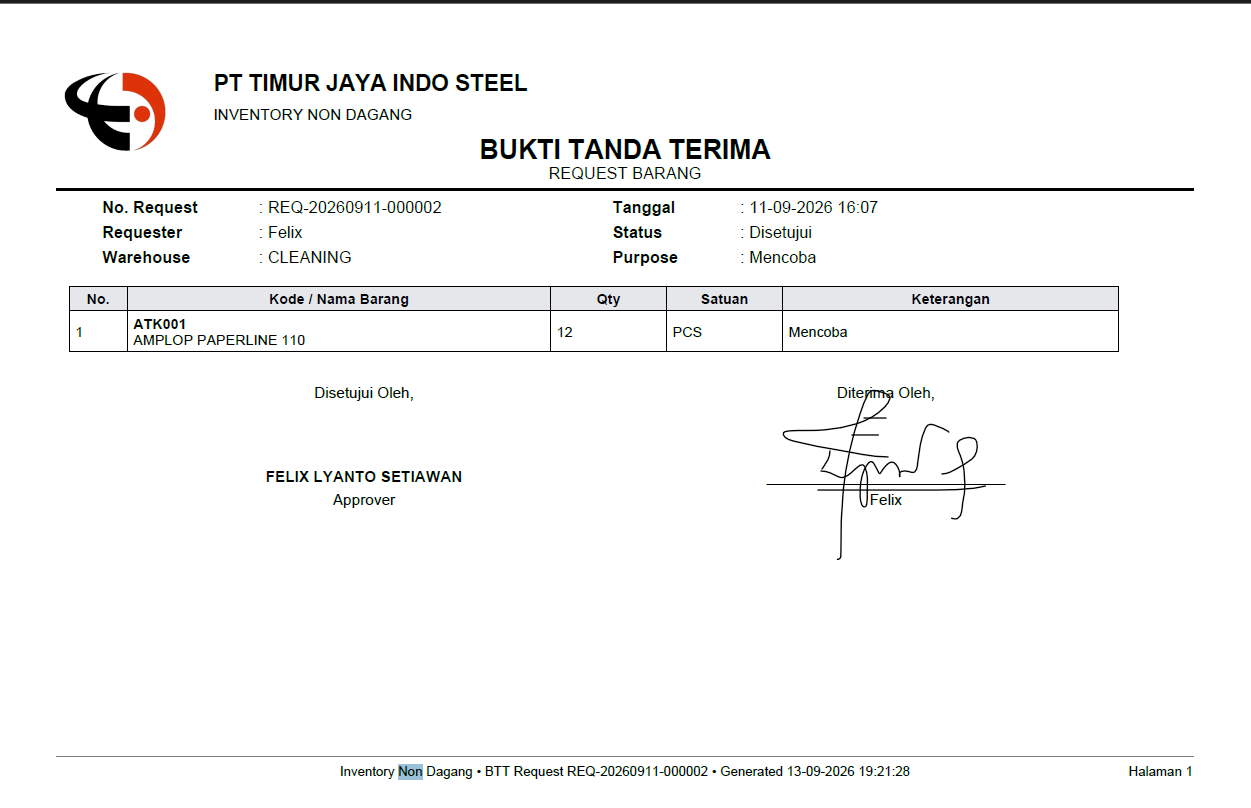
\includegraphics[
						width=0.95\linewidth,
						keepaspectratio
						]{images/GI/GI6.png}
					}
					
					\only<7>{
						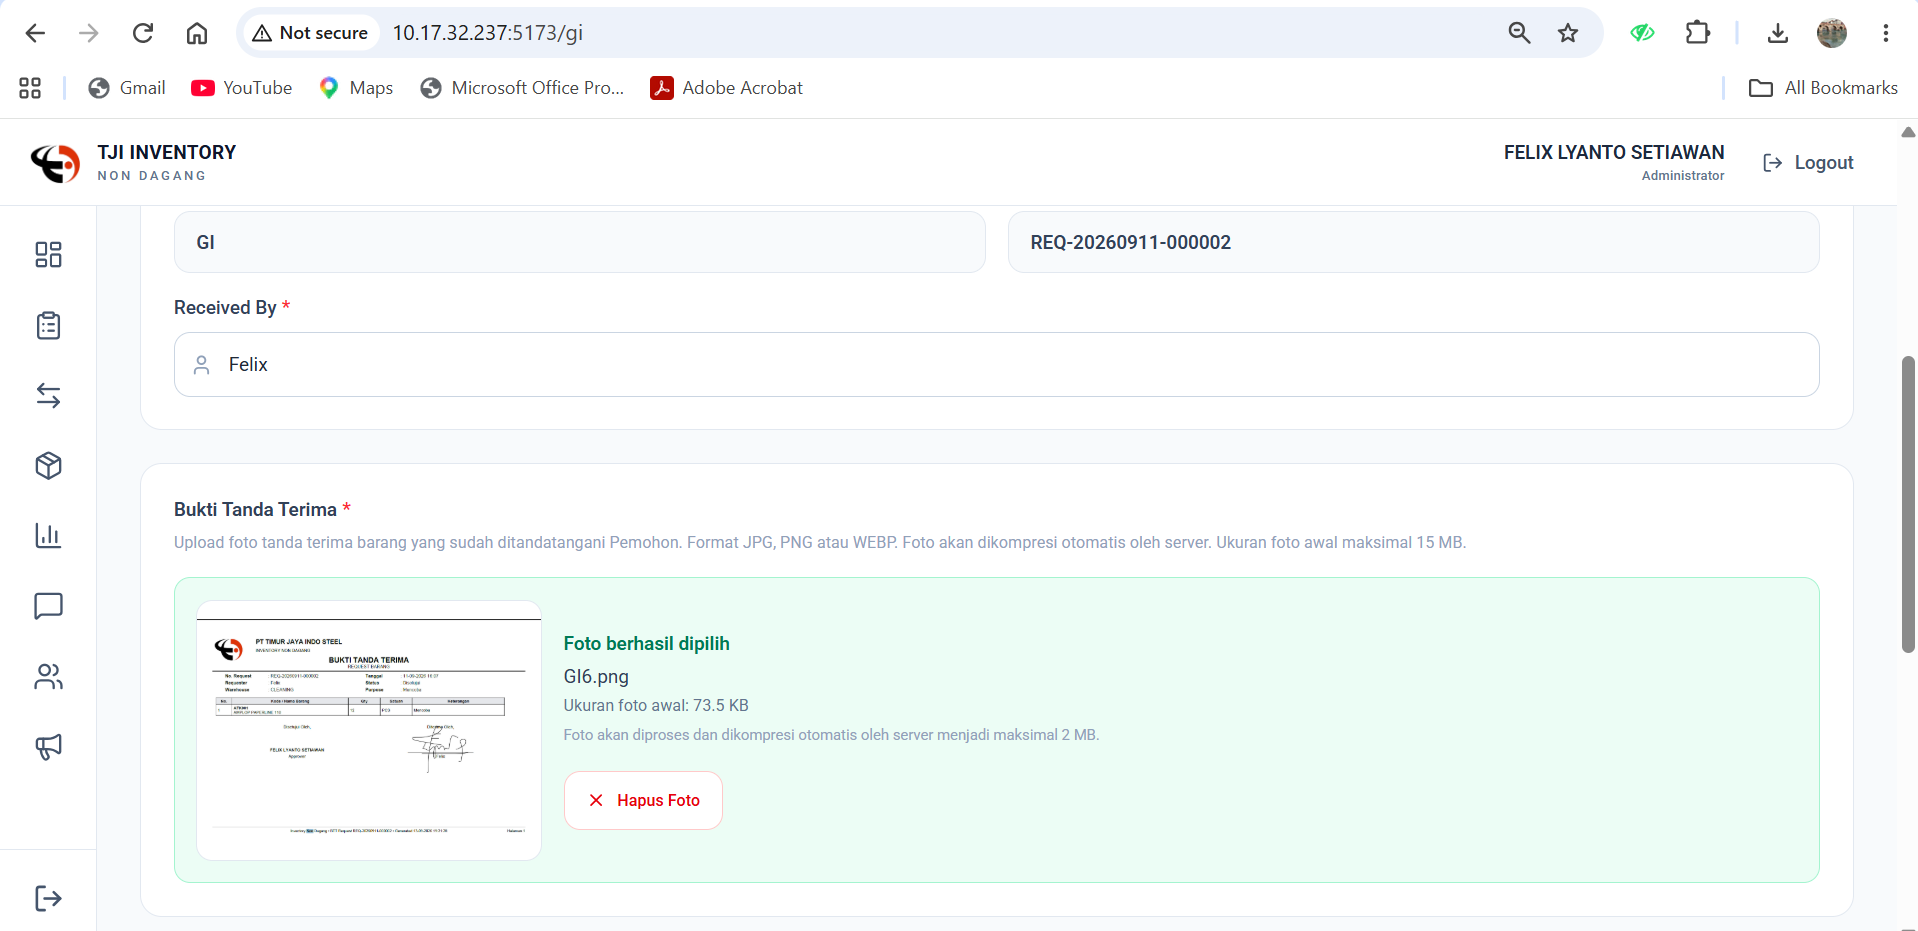
\includegraphics[
						width=0.95\linewidth,
						keepaspectratio
						]{images/GI/GI7.png}
					}
					
					\only<8>{
						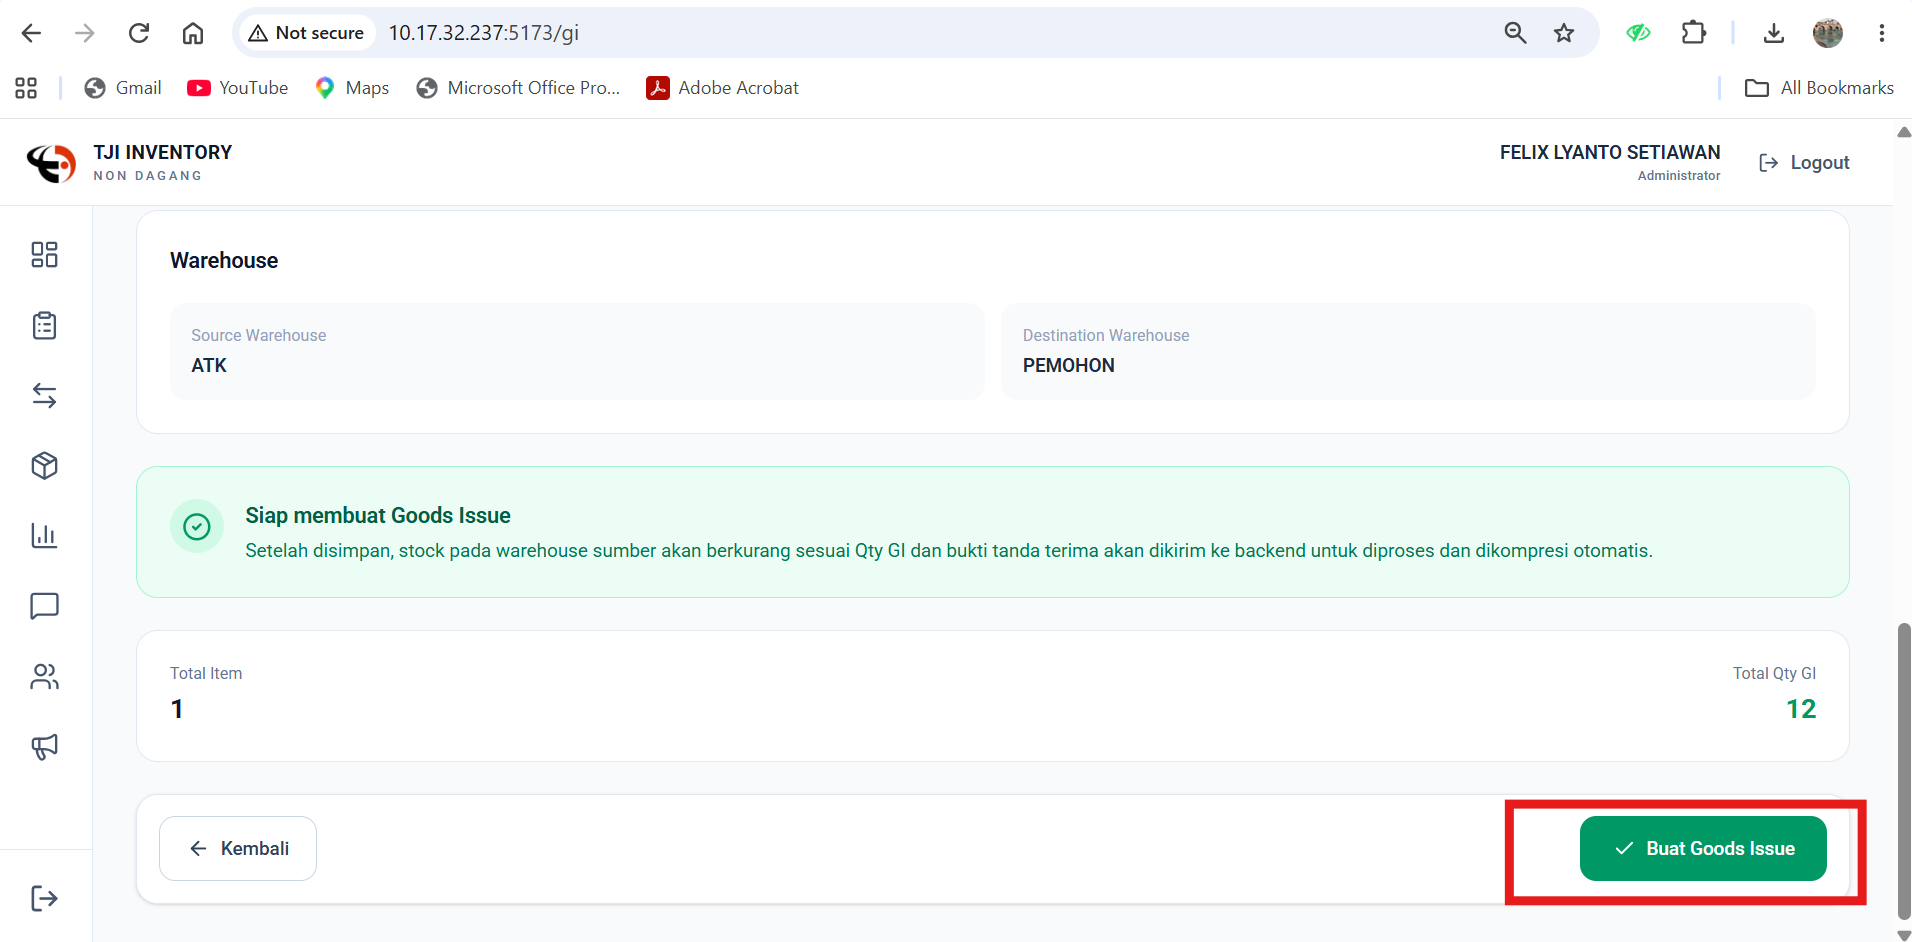
\includegraphics[
						width=0.95\linewidth,
						keepaspectratio
						]{images/GI/GI8.png}
					}
				};
				
			\end{tikzpicture}
			
		\end{center}
		
		\column{0.025\textwidth}
		
		\column{0.325\textwidth}
		
		\stepcounterdisplay{1}{8}
		\stepcounterdisplay{2}{8}
		\stepcounterdisplay{3}{8}
		\stepcounterdisplay{4}{8}
		\stepcounterdisplay{5}{8}
		\stepcounterdisplay{6}{8}
		\stepcounterdisplay{7}{8}
		\stepcounterdisplay{8}{8}
		
		\sectionlabel{Langkah}
		
		\vspace{0.08cm}
		
		\stepitem{1}{1}{
			Pilih \textbf{Transaction} $>$ \textbf{Goods Issue}.
		}
		
		\vspace{\TutorialGap}
		
		\stepitem{2}{2}{
			Pilih request yang akan diproses.
		}
		
		\vspace{\TutorialGap}
		
		\stepitem{3}{3}{
			Periksa data request dan barang yang akan dikeluarkan,
			pastikan jumlah QTY GI dan Request/Outstanding sama.
		}
		
		\vspace{\TutorialGap}
		
		\stepitem{4}{4}{
			Pilih \textbf{Review} (periksa kembali), kemudian pilih
			\textbf{Lanjut Konfirmasi}.
		}
		
		\vspace{\TutorialGap}
		
		\stepitem{5}{5}{
			Isi kolom \textbf{Received By} dengan nama penerima barang.
		}
		
		\vspace{\TutorialGap}
		
		\stepitem{6}{6}{
			Siapkan dokumen Tanda Terima yang telah
			ditandatangani oleh pemohon sebagai bukti
			serah terima barang.
		}
		
		\vspace{\TutorialGap}
		
		\stepitem{7}{7}{
			Foto dokumen Tanda Terima (untuk Android) /
			Upload foto Tanda Terima (untuk Desktop).
		}
		
		\vspace{\TutorialGap}
		
		\stepitem{8}{8}{
			Pilih \textbf{Posting Goods Issue} untuk menyelesaikan
			proses pengeluaran barang.
		}
		
	\end{columns}
	
\end{frame}
	



\begin{frame}{05 --- Goods Receipt (Penerimaan Barang)}
	
	\vspace{-0.25cm}
	
	\begin{columns}[T,totalwidth=\textwidth]
		
		\column{0.65\textwidth}
		
		\begin{center}
			
			\begin{tikzpicture}
				
				\node[
				inner sep=0,
				outer sep=0
				] (screen)
				{
					\only<1>{
						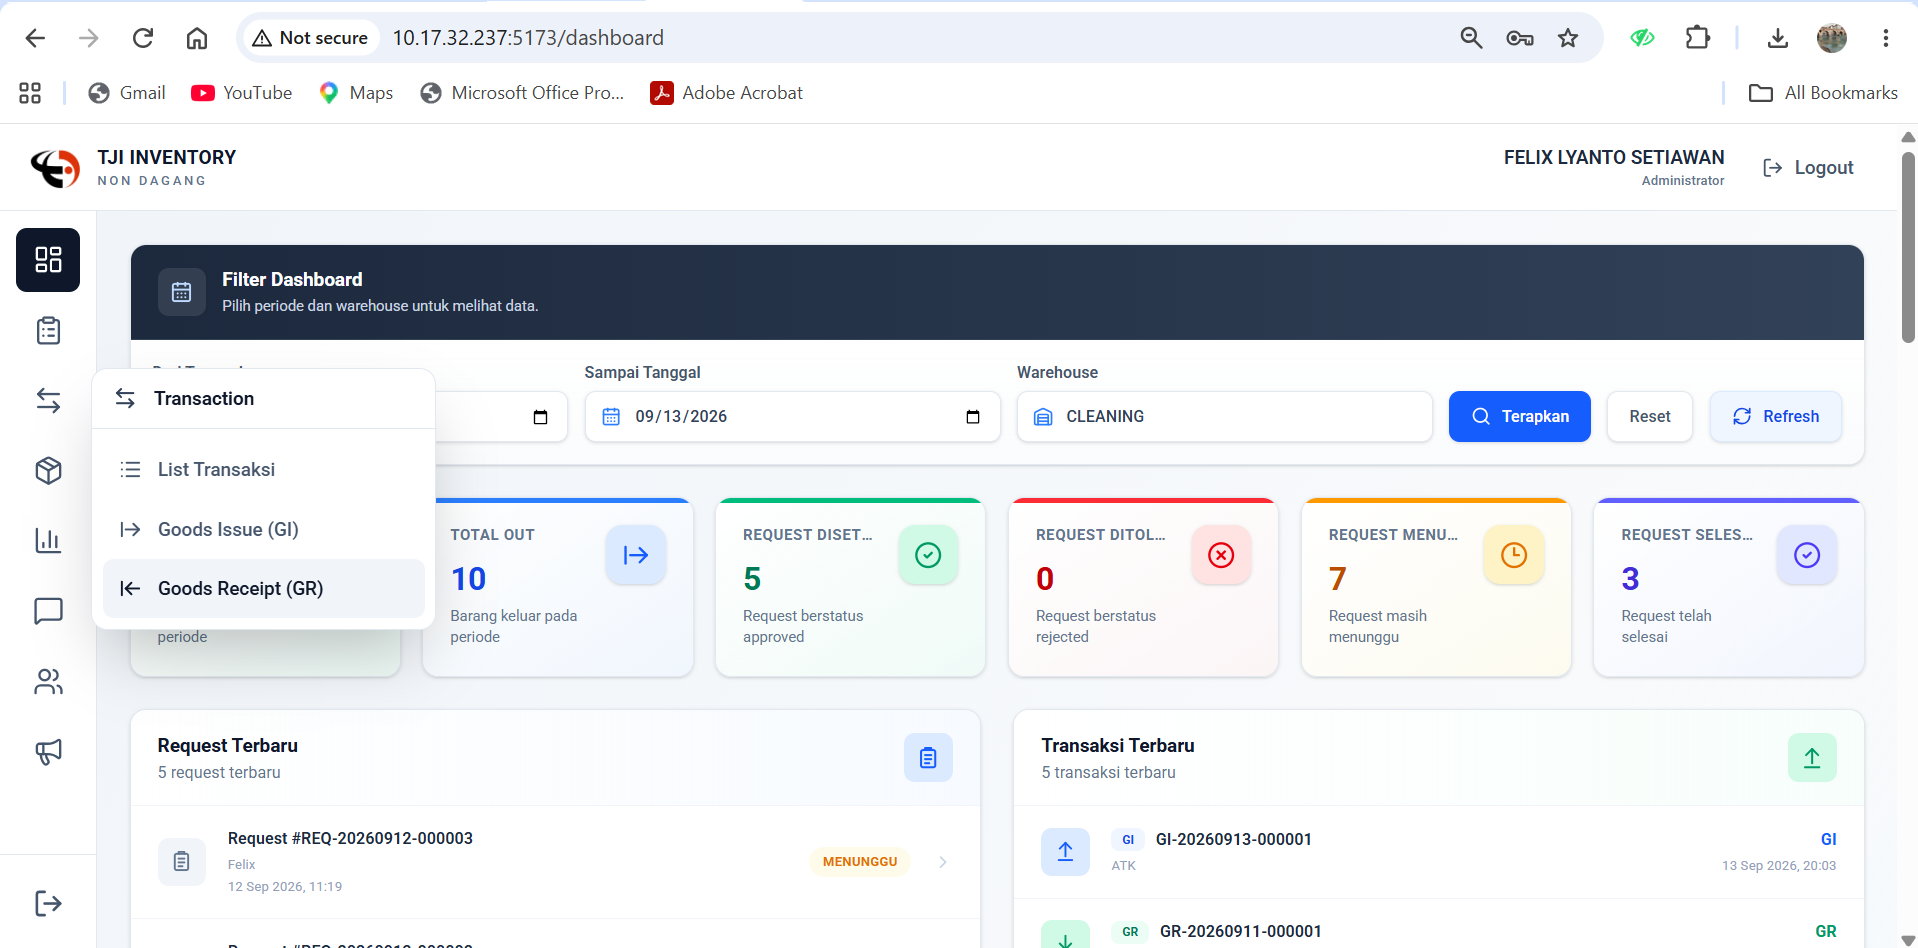
\includegraphics[
						width=0.95\linewidth,
						keepaspectratio
						]{images/GR/GR1.png}
					}
					
					\only<2>{
						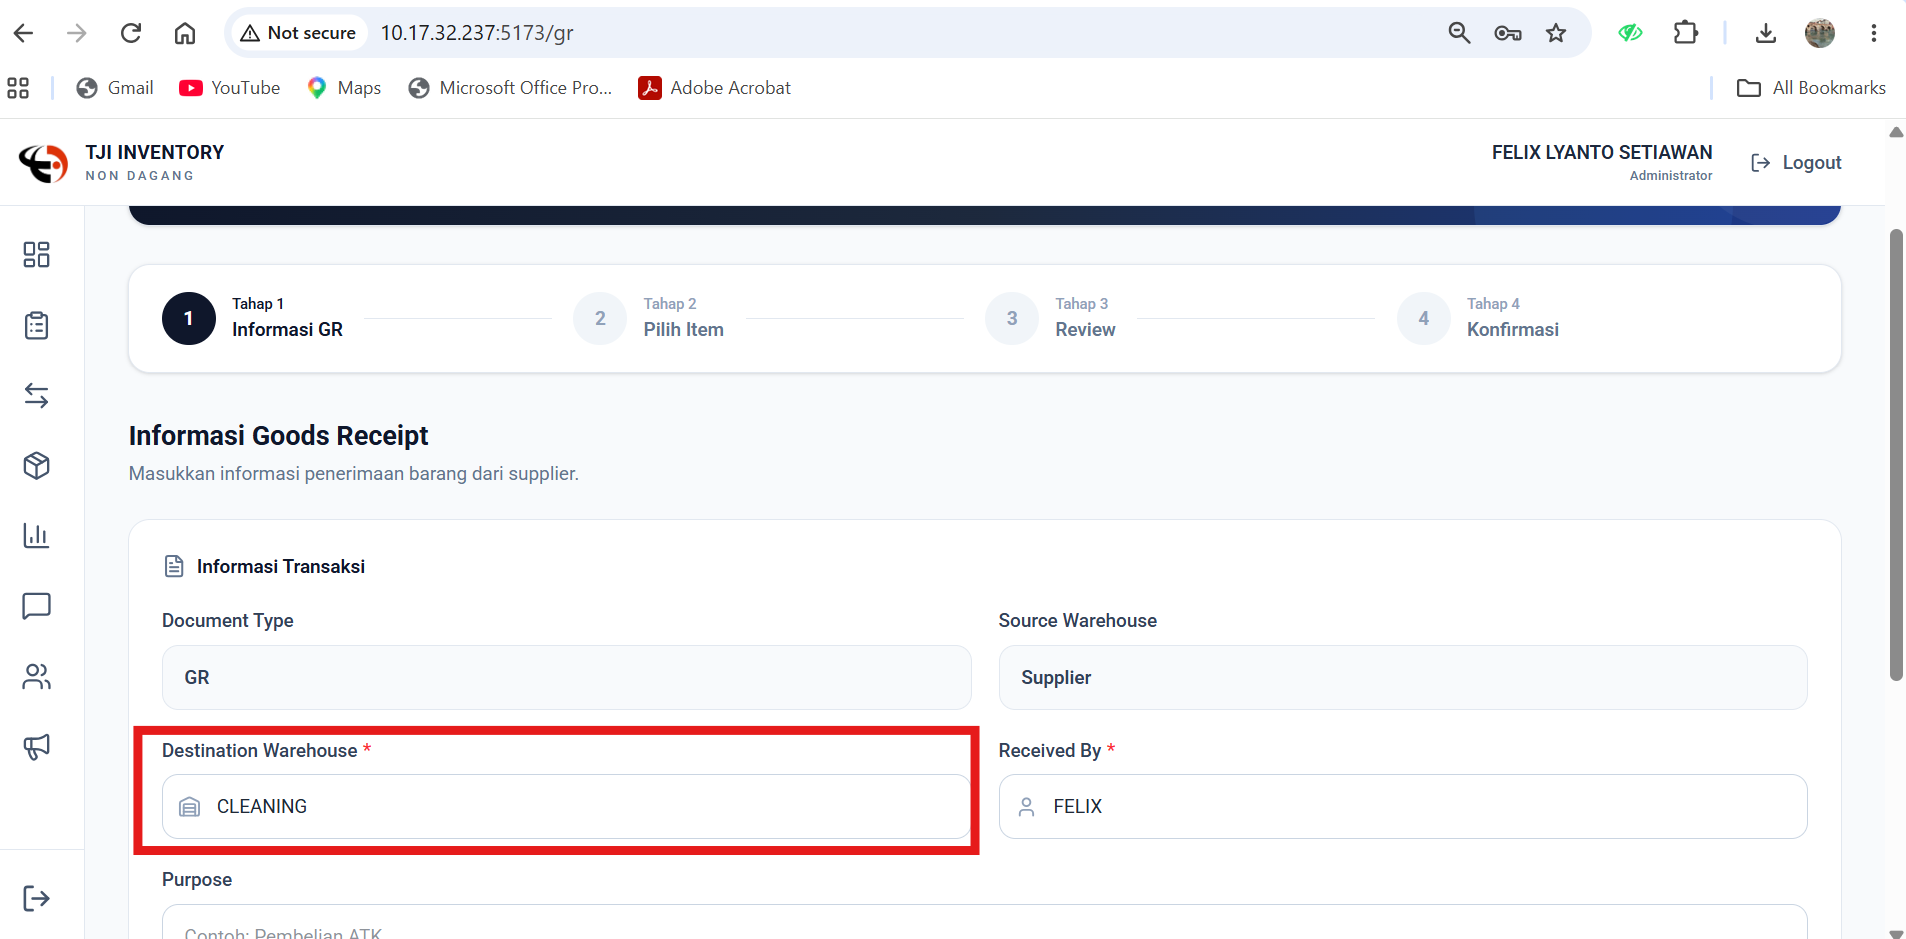
\includegraphics[
						width=0.95\linewidth,
						keepaspectratio
						]{images/GR/GR2.png}
					}
					
					\only<3>{
						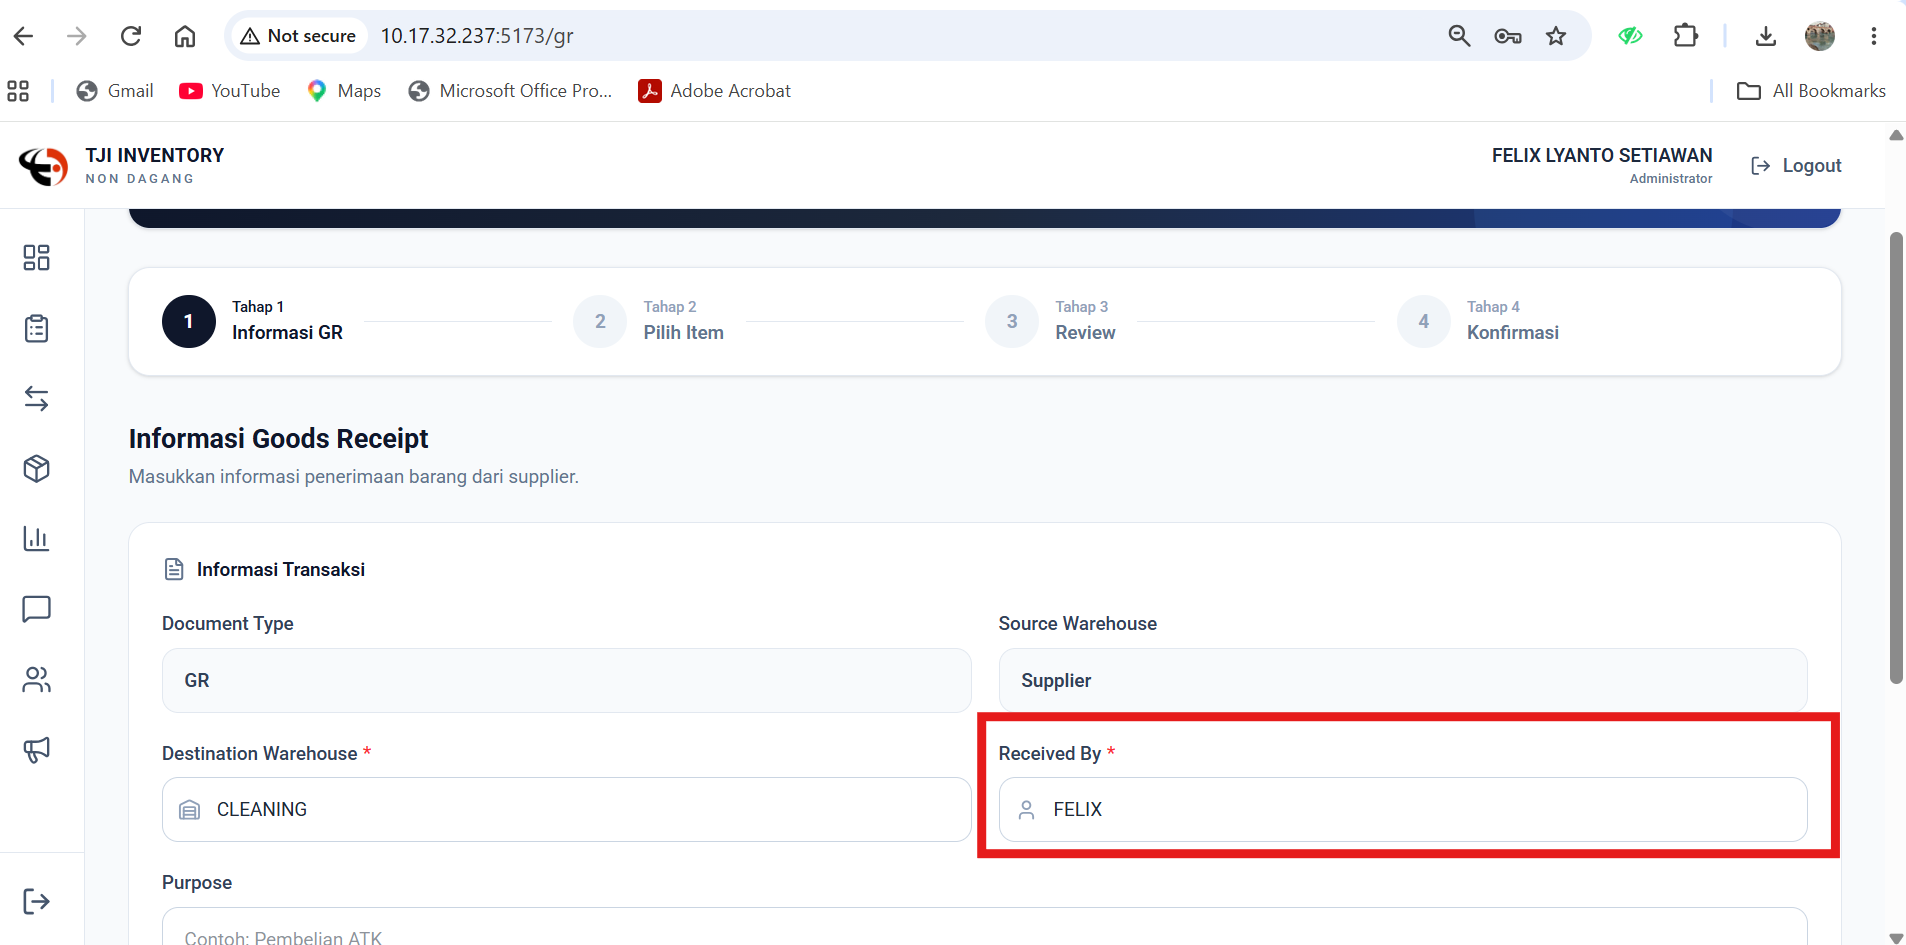
\includegraphics[
						width=0.95\linewidth,
						keepaspectratio
						]{images/GR/GR3.png}
					}
					
					\only<4>{
						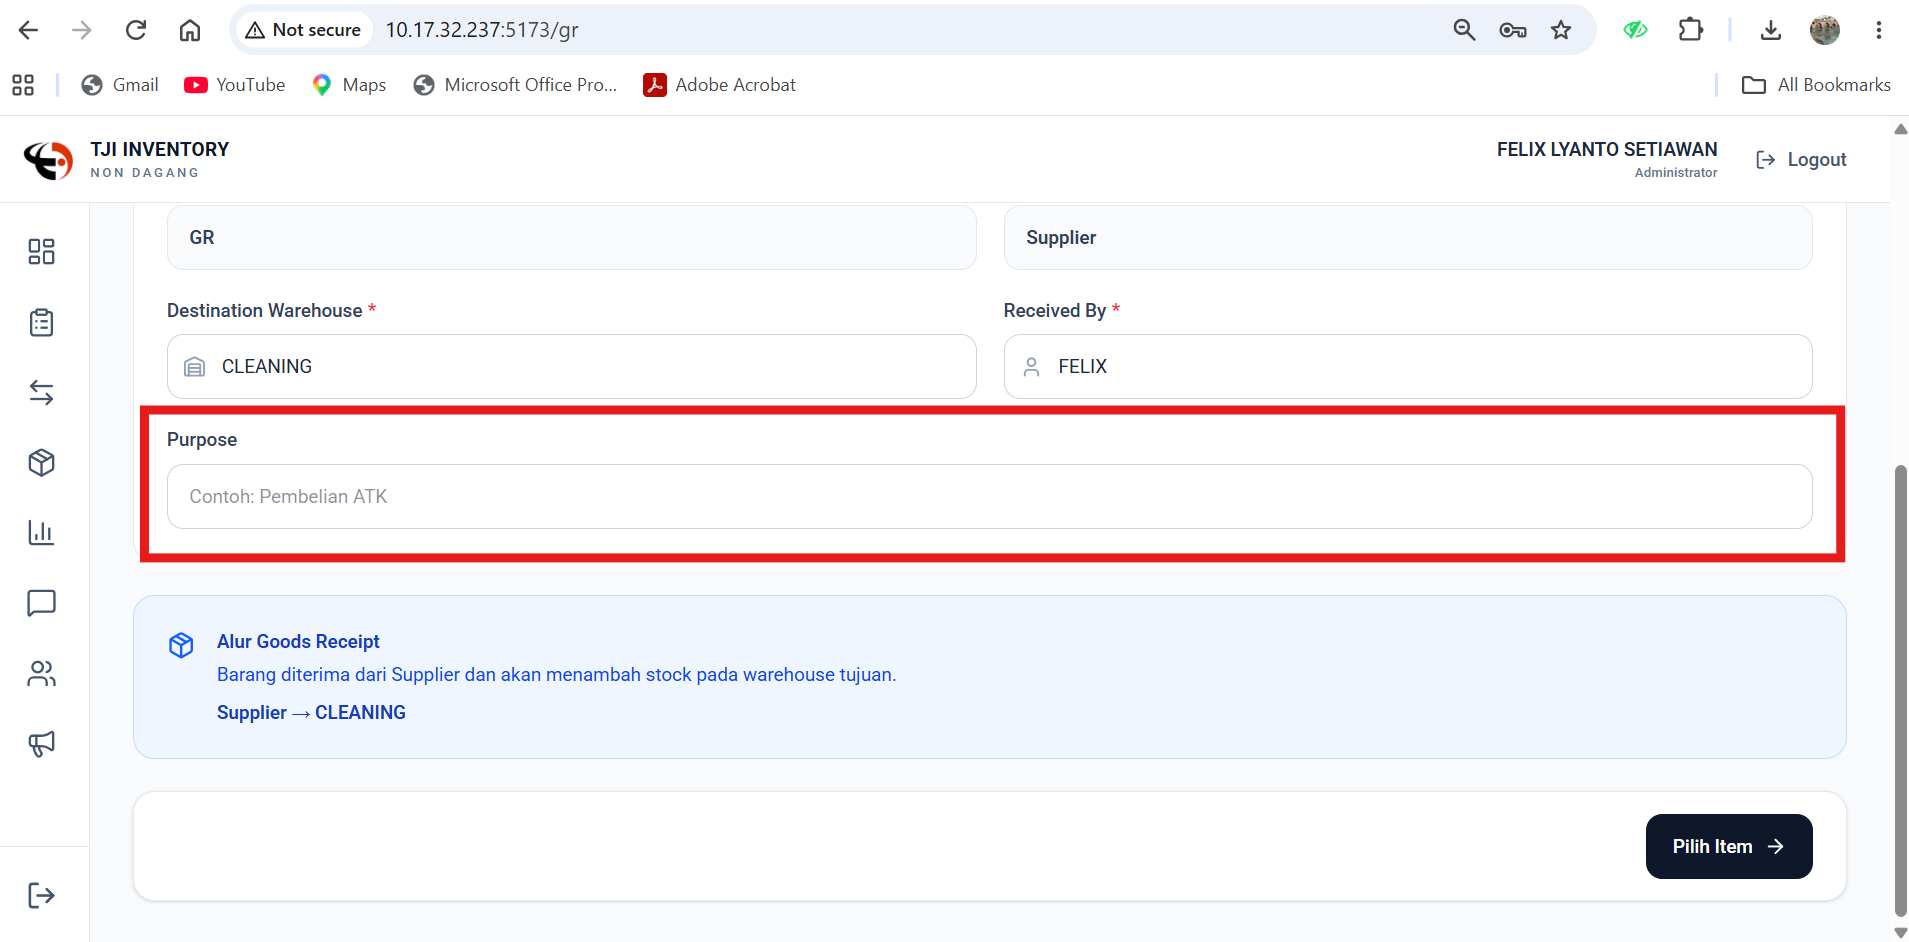
\includegraphics[
						width=0.95\linewidth,
						keepaspectratio
						]{images/GR/GR4.png}
					}
					
					\only<5>{
						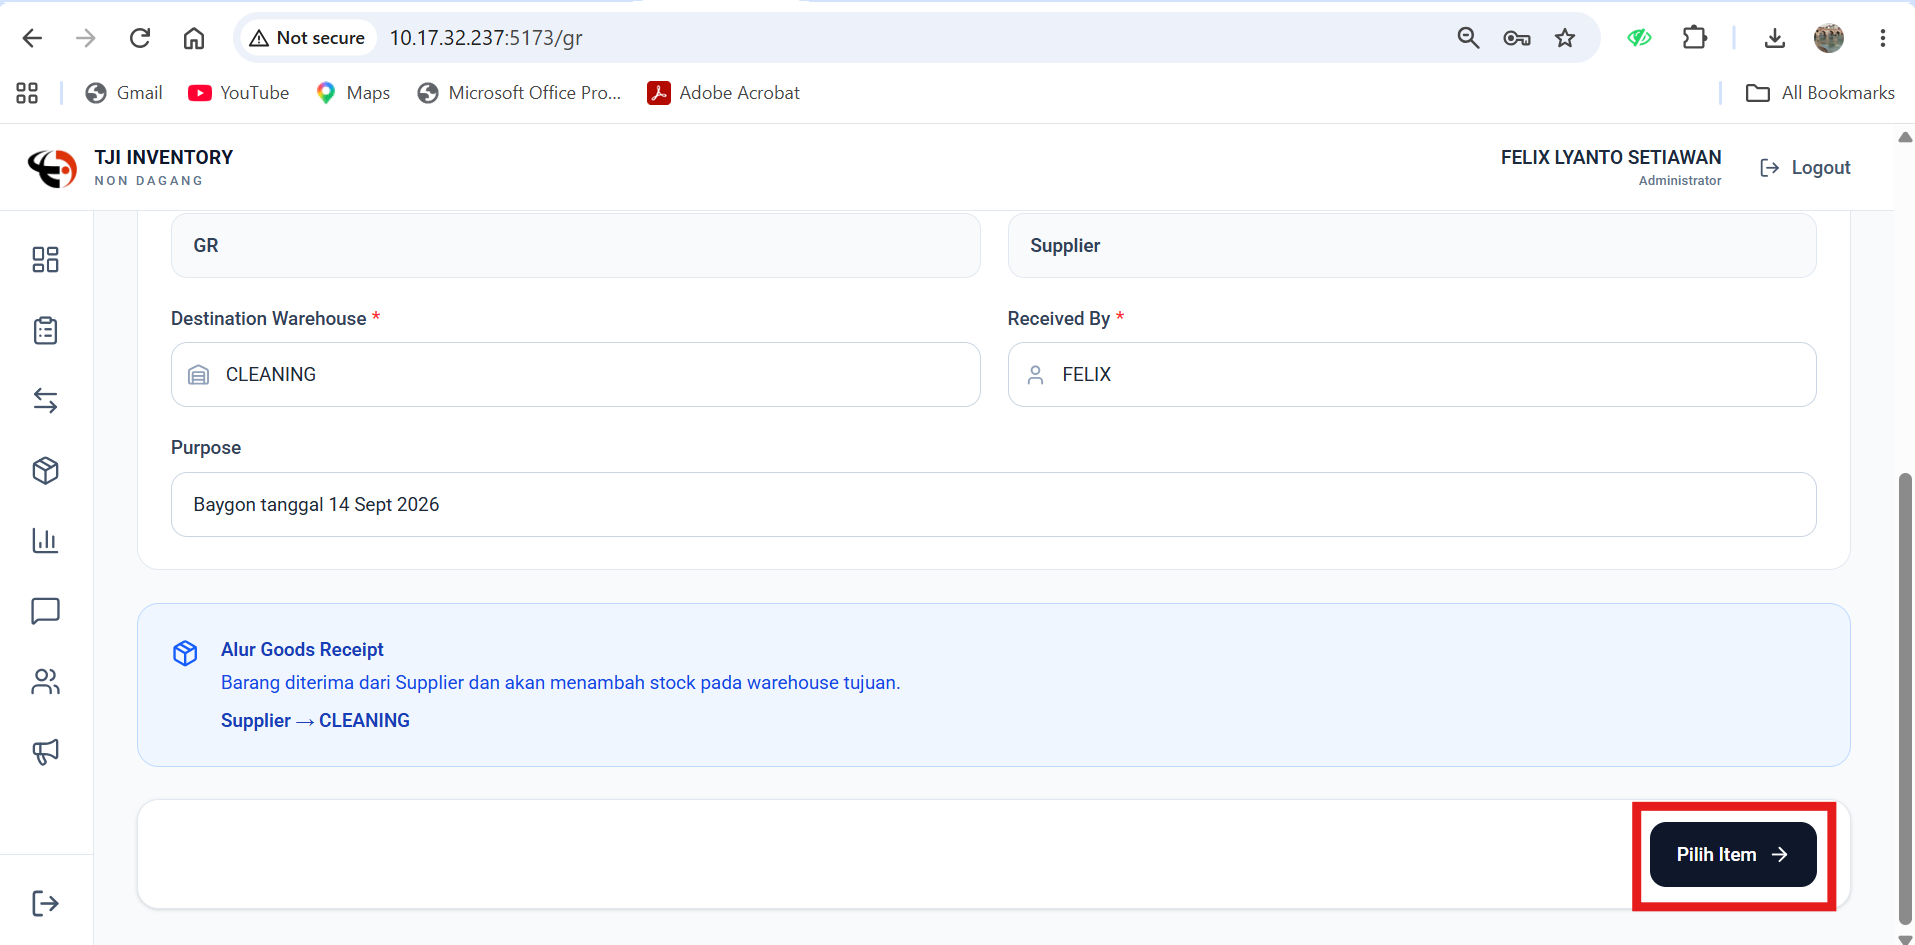
\includegraphics[
						width=0.95\linewidth,
						keepaspectratio
						]{images/GR/GR5.png}
					}
					
					\only<6>{
						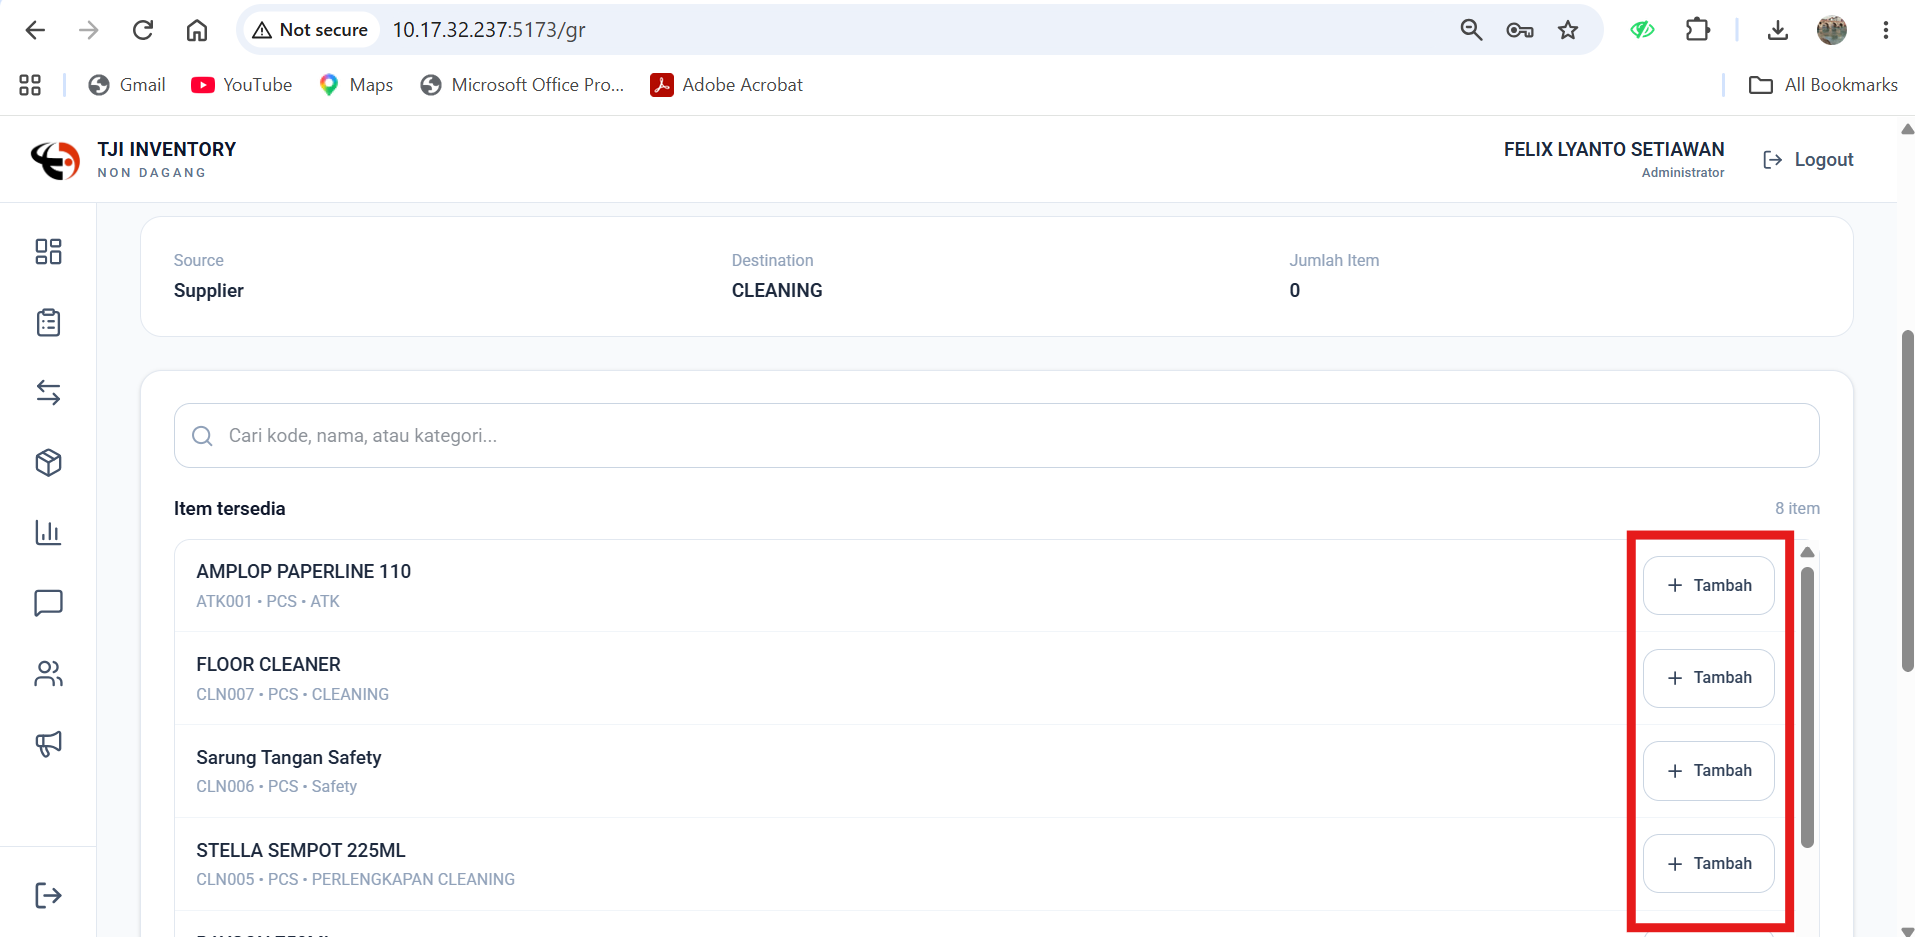
\includegraphics[
						width=0.95\linewidth,
						keepaspectratio
						]{images/GR/GR6.png}
					}
					
					\only<7>{
						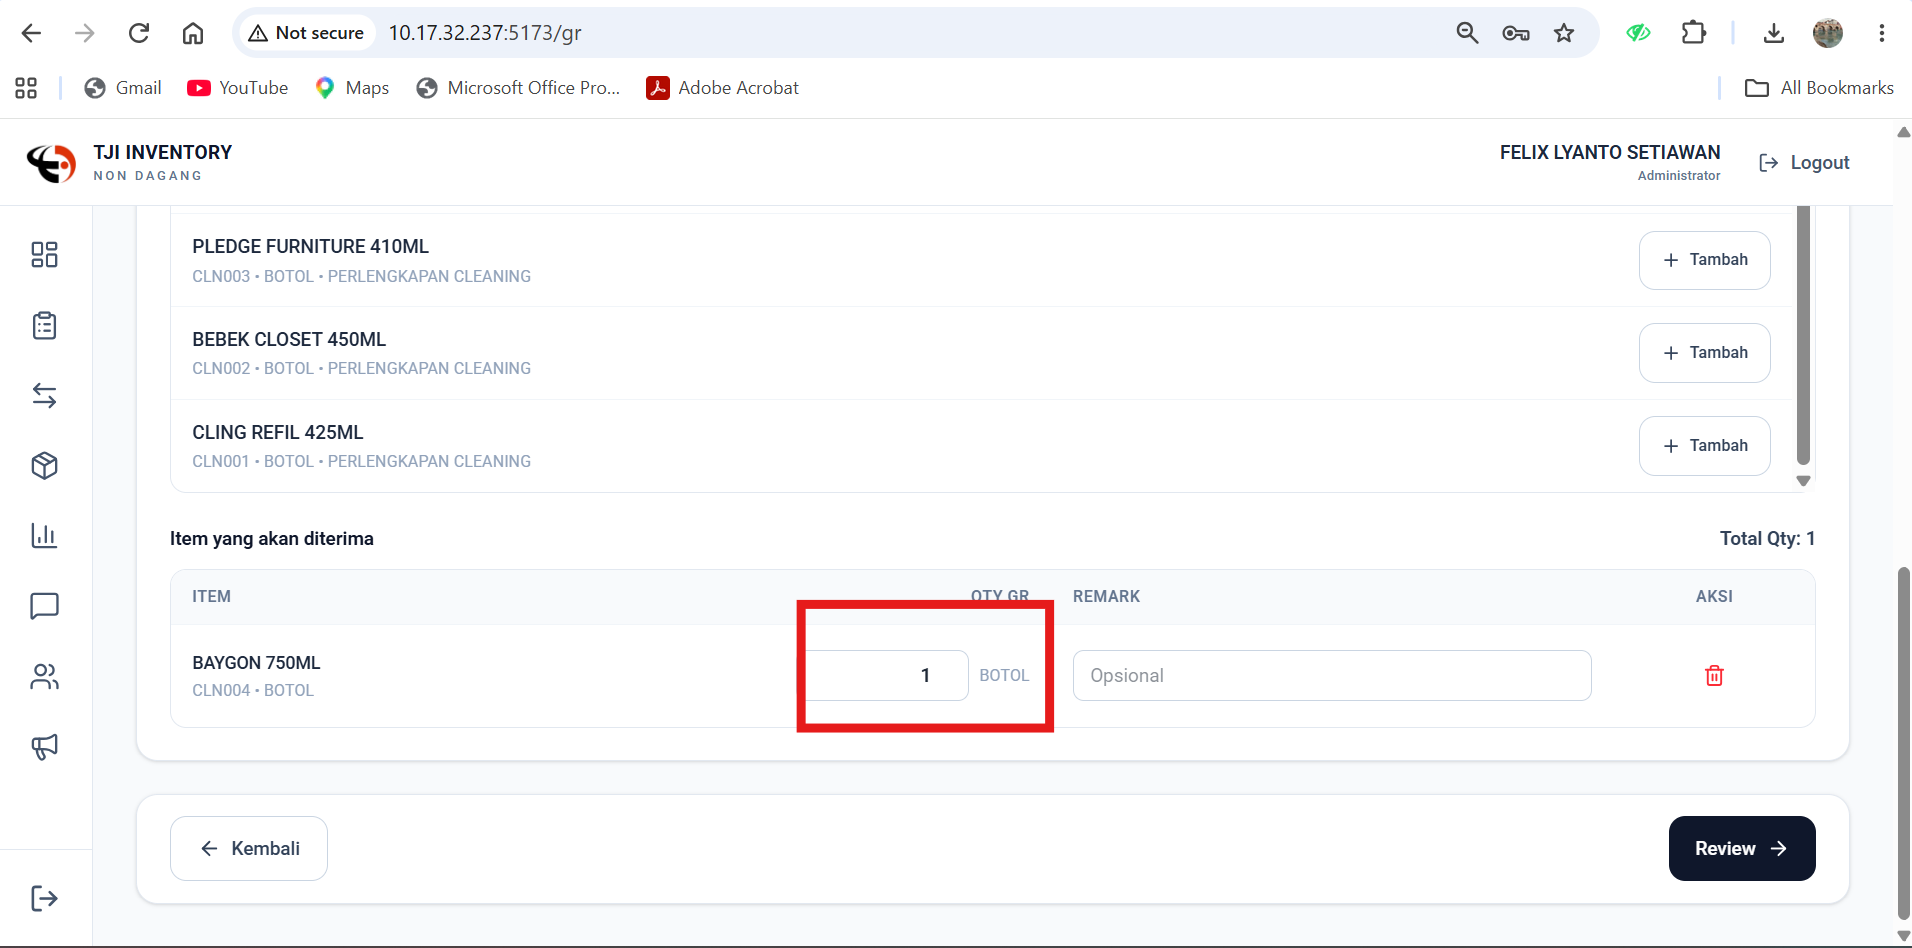
\includegraphics[
						width=0.95\linewidth,
						keepaspectratio
						]{images/GR/GR7.png}
					}
					
					\only<8>{
						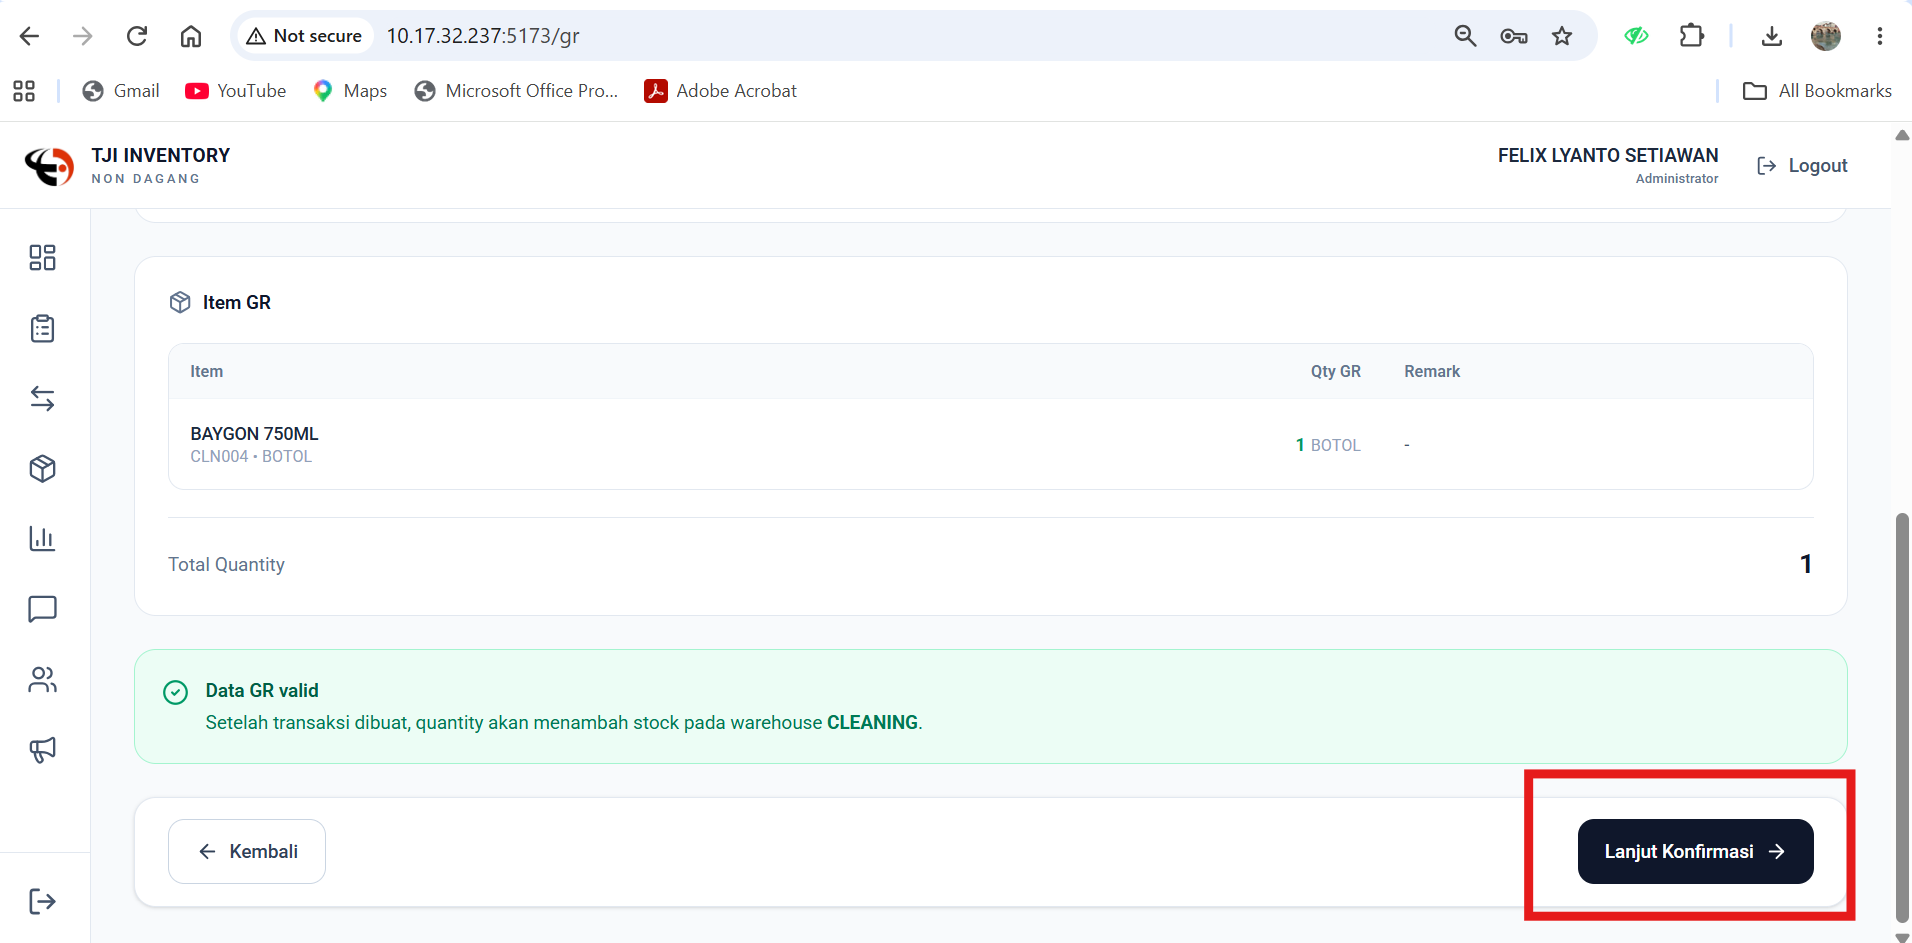
\includegraphics[
						width=0.95\linewidth,
						keepaspectratio
						]{images/GR/GR8.png}
					}
					
					\only<9>{
						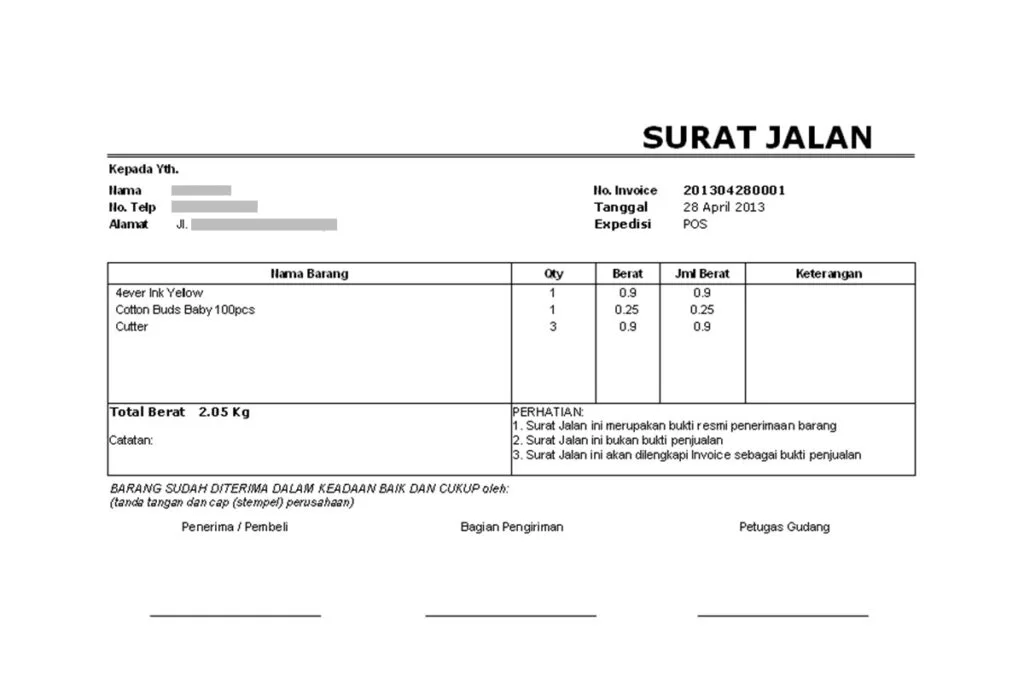
\includegraphics[
						width=0.95\linewidth,
						keepaspectratio
						]{images/GR/GR9.png}
					}
					
					\only<10>{
						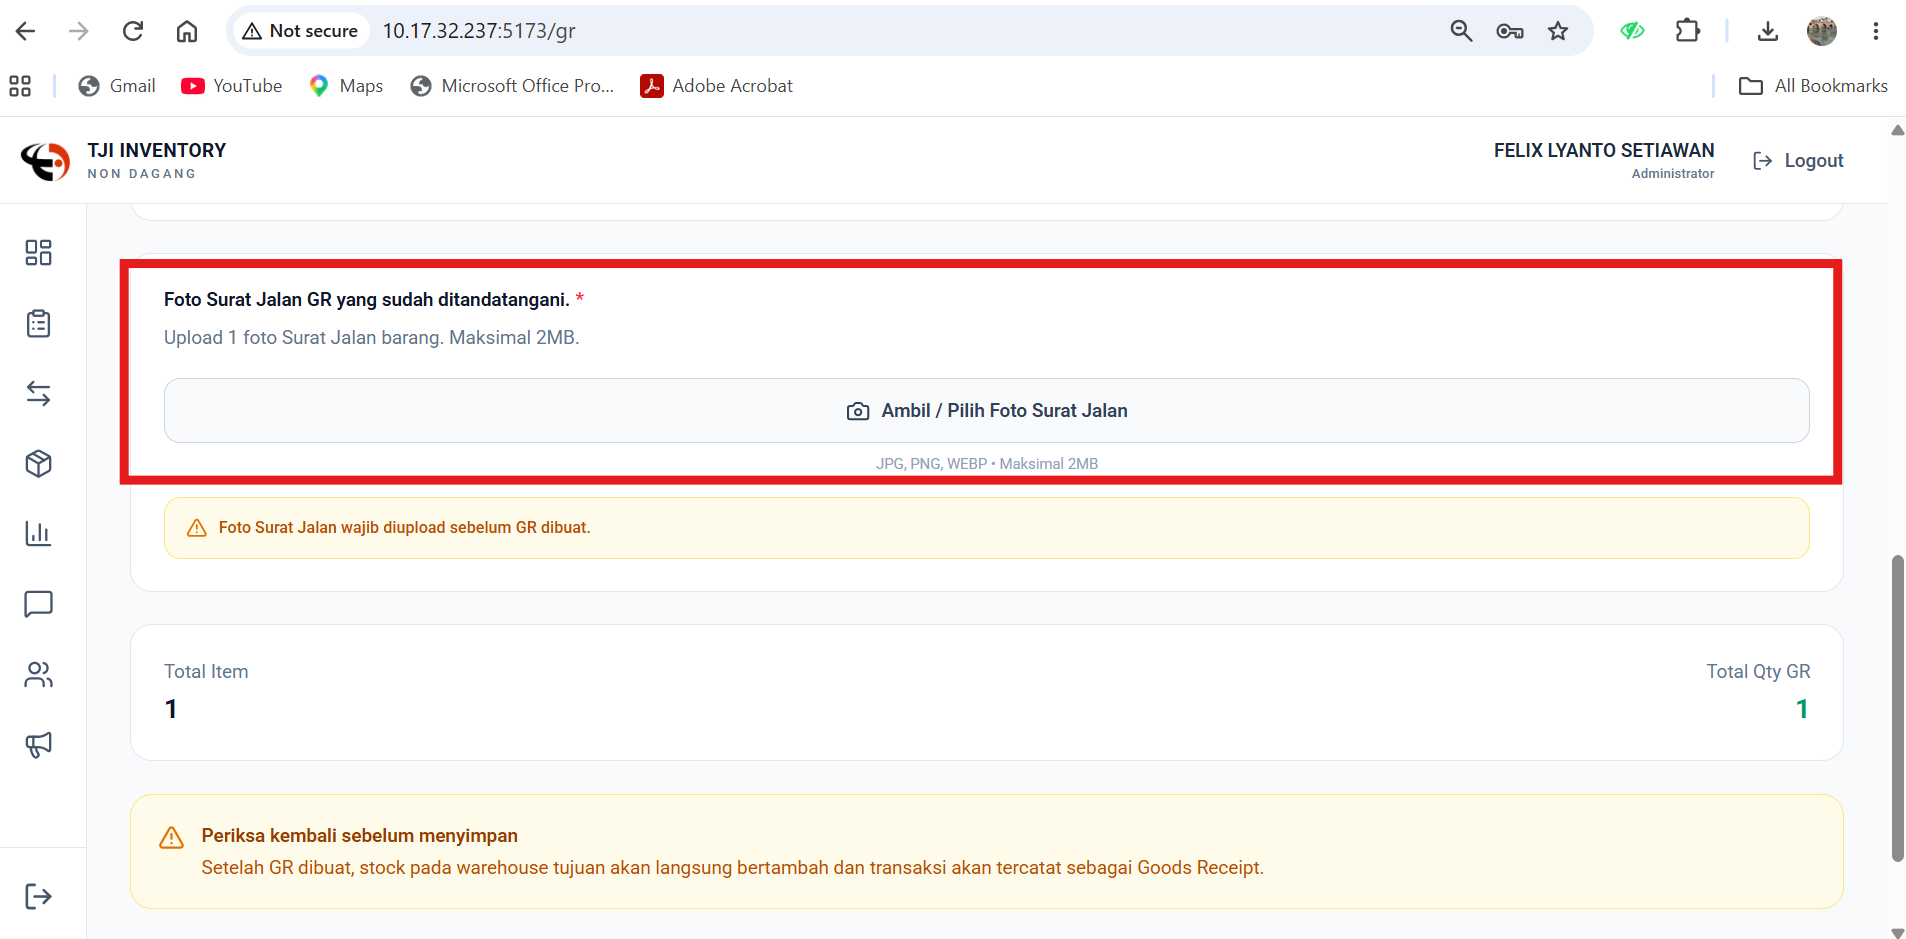
\includegraphics[
						width=0.95\linewidth,
						keepaspectratio
						]{images/GR/GR10.png}
					}
					
					\only<11>{
						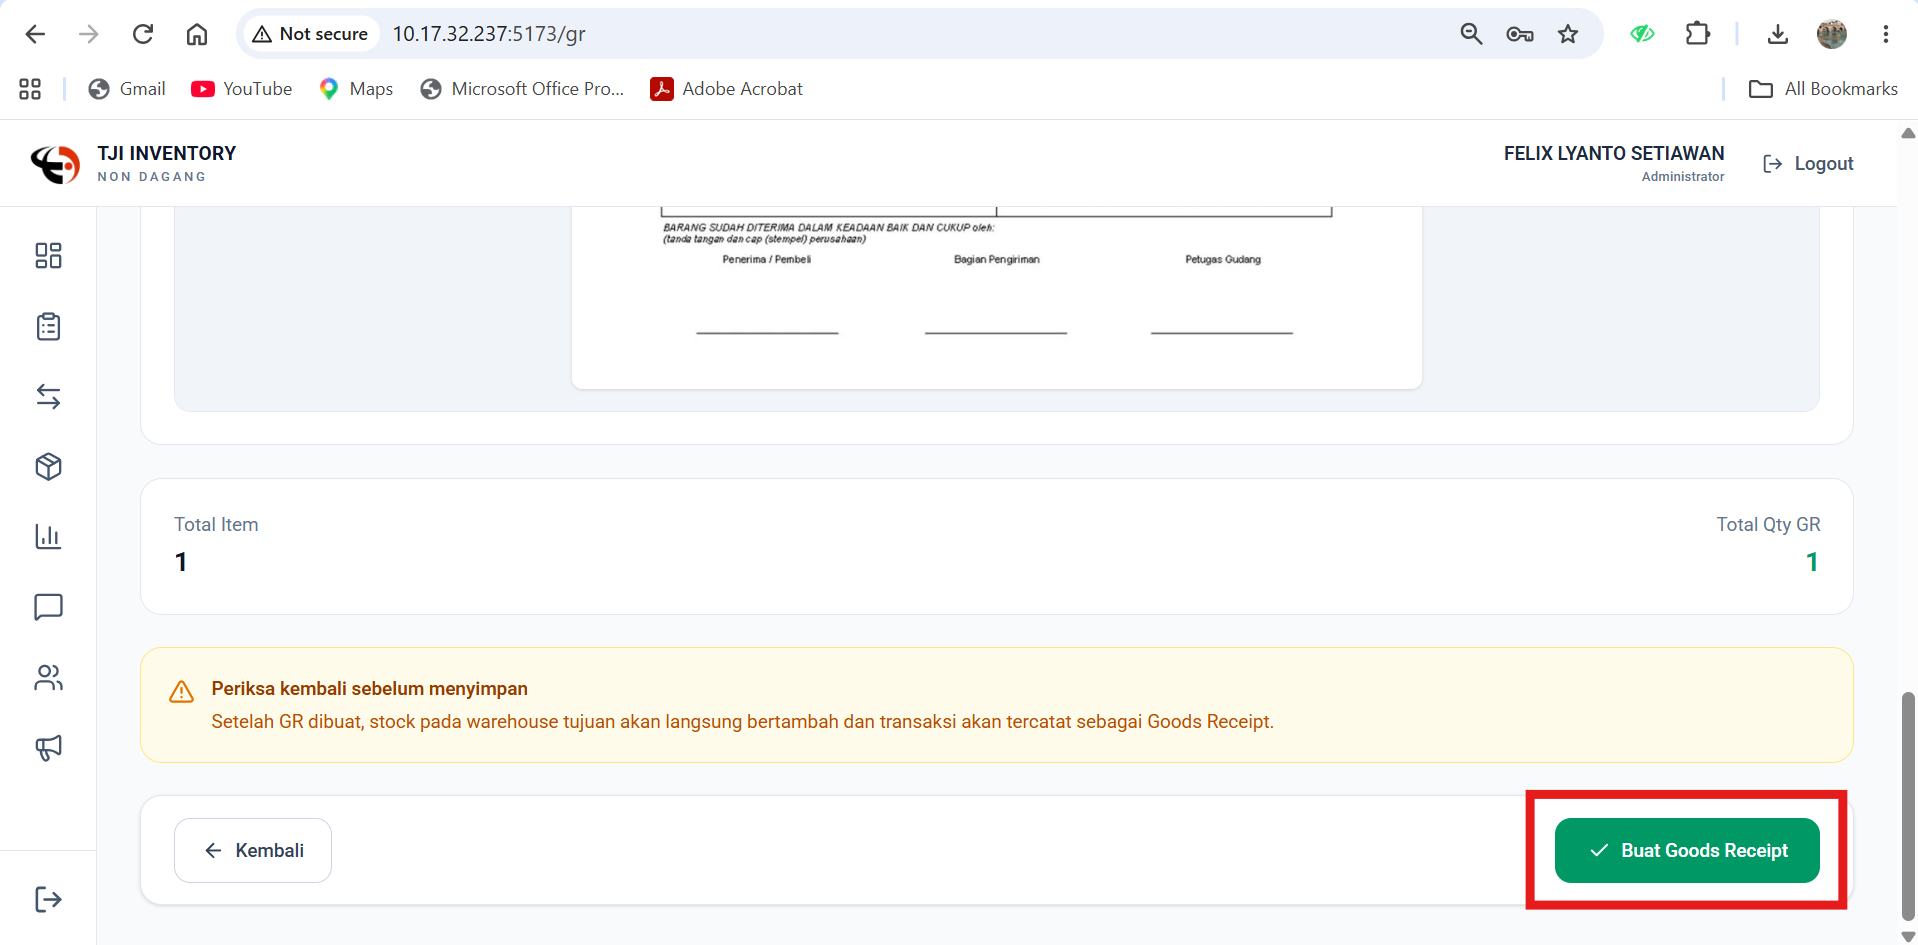
\includegraphics[
						width=0.95\linewidth,
						keepaspectratio
						]{images/GR/GR11.png}
					}
				};
				
			\end{tikzpicture}
			
		\end{center}
		
		\column{0.025\textwidth}
		
		\column{0.325\textwidth}
		
		\stepcounterdisplay{1}{11}
		\stepcounterdisplay{2}{11}
		\stepcounterdisplay{3}{11}
		\stepcounterdisplay{4}{11}
		\stepcounterdisplay{5}{11}
		\stepcounterdisplay{6}{11}
		\stepcounterdisplay{7}{11}
		\stepcounterdisplay{8}{11}
		\stepcounterdisplay{9}{11}
		\stepcounterdisplay{10}{11}
		\stepcounterdisplay{11}{11}
		
		\sectionlabel{Langkah}
		
		\vspace{0.08cm}
		
		\stepitem{1}{1}{
			Pilih \textbf{Transaction} $>$ \textbf{Goods Receipt}.
		}
		
		\vspace{\TutorialGap}
		
		\stepitem{2}{2}{
			Pilih \textbf{Destination Warehouse} sebagai
			lokasi tujuan penerimaan barang, sesuai kategori barang.
		}
		
		\vspace{\TutorialGap}
		
		\stepitem{3}{3}{
			Isi nama penerima barang
			pada kolom \textbf{Received By}.
		}
		
		\vspace{\TutorialGap}
		
		\stepitem{4}{4}{
			Isi kolom \textbf{Purpose}
			untuk mempermudah pengecekan.
		}
		
		\vspace{\TutorialGap}
		
		\stepitem{5}{5}{
			Masuk ke \textbf{Pilih Item}.
		}
		
		\vspace{\TutorialGap}
		
		\stepitem{6}{6}{
			Pilih \textbf{+ Tambah} sesuai dengan barang
			yang diterima. Dapat memilih lebih dari 1 item,
			namun harus dalam satu warehouse.
		}
		
		\vspace{\TutorialGap}
		
		\stepitem{7}{7}{
			Isi jumlah barang yang diterima serta
			isi \textbf{Remark} jika diperlukan.
		}
		
		\vspace{\TutorialGap}
		
		\stepitem{8}{8}{
			Periksa kembali detail data penerimaan barang,
			kemudian pilih \textbf{Lanjut Konfirmasi}.
		}
		
		\vspace{\TutorialGap}
		
		\stepitem{9}{9}{
			Siapkan dokumen Surat Jalan yang dari Supplier.
		}
		
		\vspace{\TutorialGap}
		
		\stepitem{10}{10}{
			Foto dokumen Surat Jalan (untuk Android) /
			Upload foto Surat Jalan (untuk Desktop).
		}
		
		\vspace{\TutorialGap}
		
		\stepitem{11}{11}{
			Periksa kembali seluruh data Goods Receipt,
			kemudian \textbf{Pilih Buat Goods Receipt}.
		}
		
	\end{columns}
	
\end{frame}

\begin{frame}{Attention}
	
	\vfill
	
	\begin{center}
		
		\begin{minipage}{0.90\textwidth}
			
			\warningbox{Perlu Diperhatikan}{
				\large
				\begin{itemize}
					\item Satu Transaksi Goods Receipt hanya dapat berisi barang dari
					\textbf{satu kategori}.
					\vspace{0.15cm}
					 Contoh penerimaan BAYGON 750ML (Cleaning) tidak bisa dijadikan satu transaksi dengan AMPLOP PAPERLINE 110 (ATK).
					\item Semua barang yang dapat dilakukan permintaan, pengeluaran dan penerimaan hanya barang yang teregistrasi di \textbf{Master Item}.
					
					\vspace{0.30cm}
					
					\item Pada perangkat \textbf{Android, iOS, dan Tablet},
					bukti foto dapat diunggah langsung menggunakan kamera
					perangkat.
					
					\vspace{0.15cm}
					
					Pada versi \textbf{Desktop}, bukti foto dapat diunggah
					dalam format \textbf{JPG, PNG, atau WEBP}.
				\end{itemize}
			}
			
		\end{minipage}
		
	\end{center}
	
	\vfill
	
\end{frame}


\begin{frame}{05 --- Master Item}
	
	\vspace{-0.25cm}
	
	\begin{columns}[T,totalwidth=\textwidth]
		
		\column{0.65\textwidth}
		
		\begin{center}
			
			\begin{tikzpicture}
				
				\node[
				inner sep=0,
				outer sep=0
				] (screen)
				{
					\only<1>{
						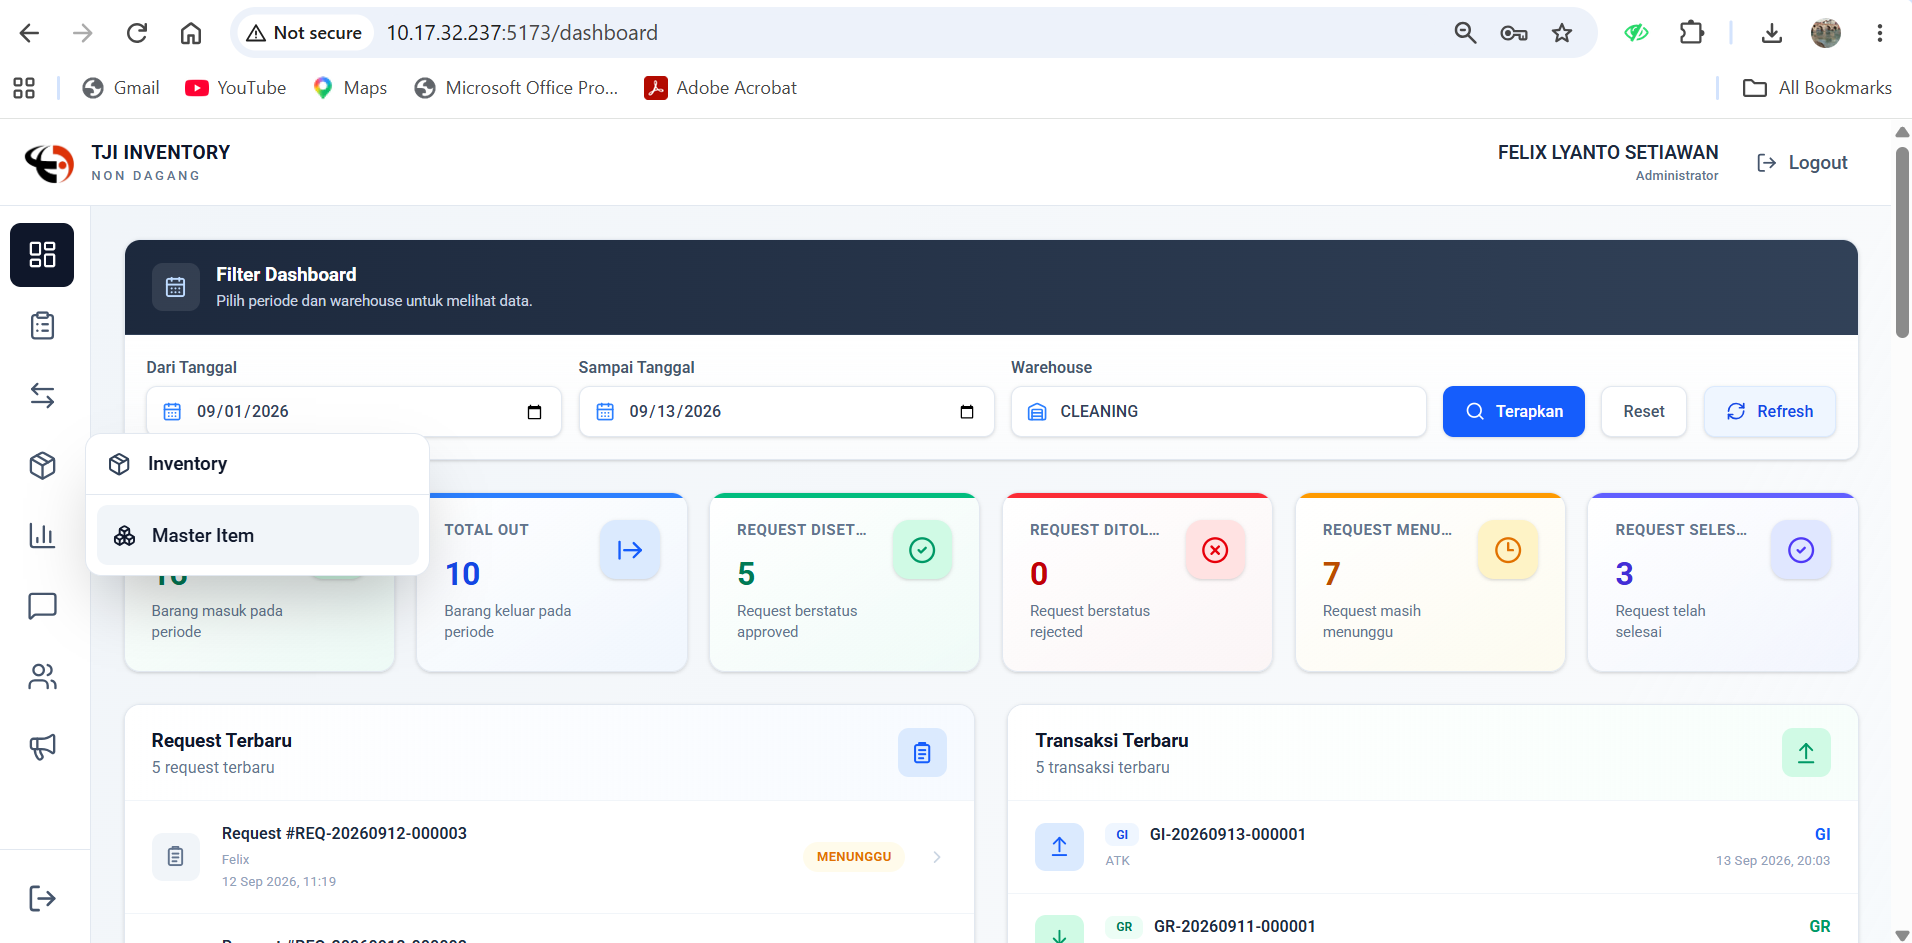
\includegraphics[
						width=0.95\linewidth,
						keepaspectratio
						]{images/Master Item/CreateItem1.png}
					}
					
					\only<2>{
						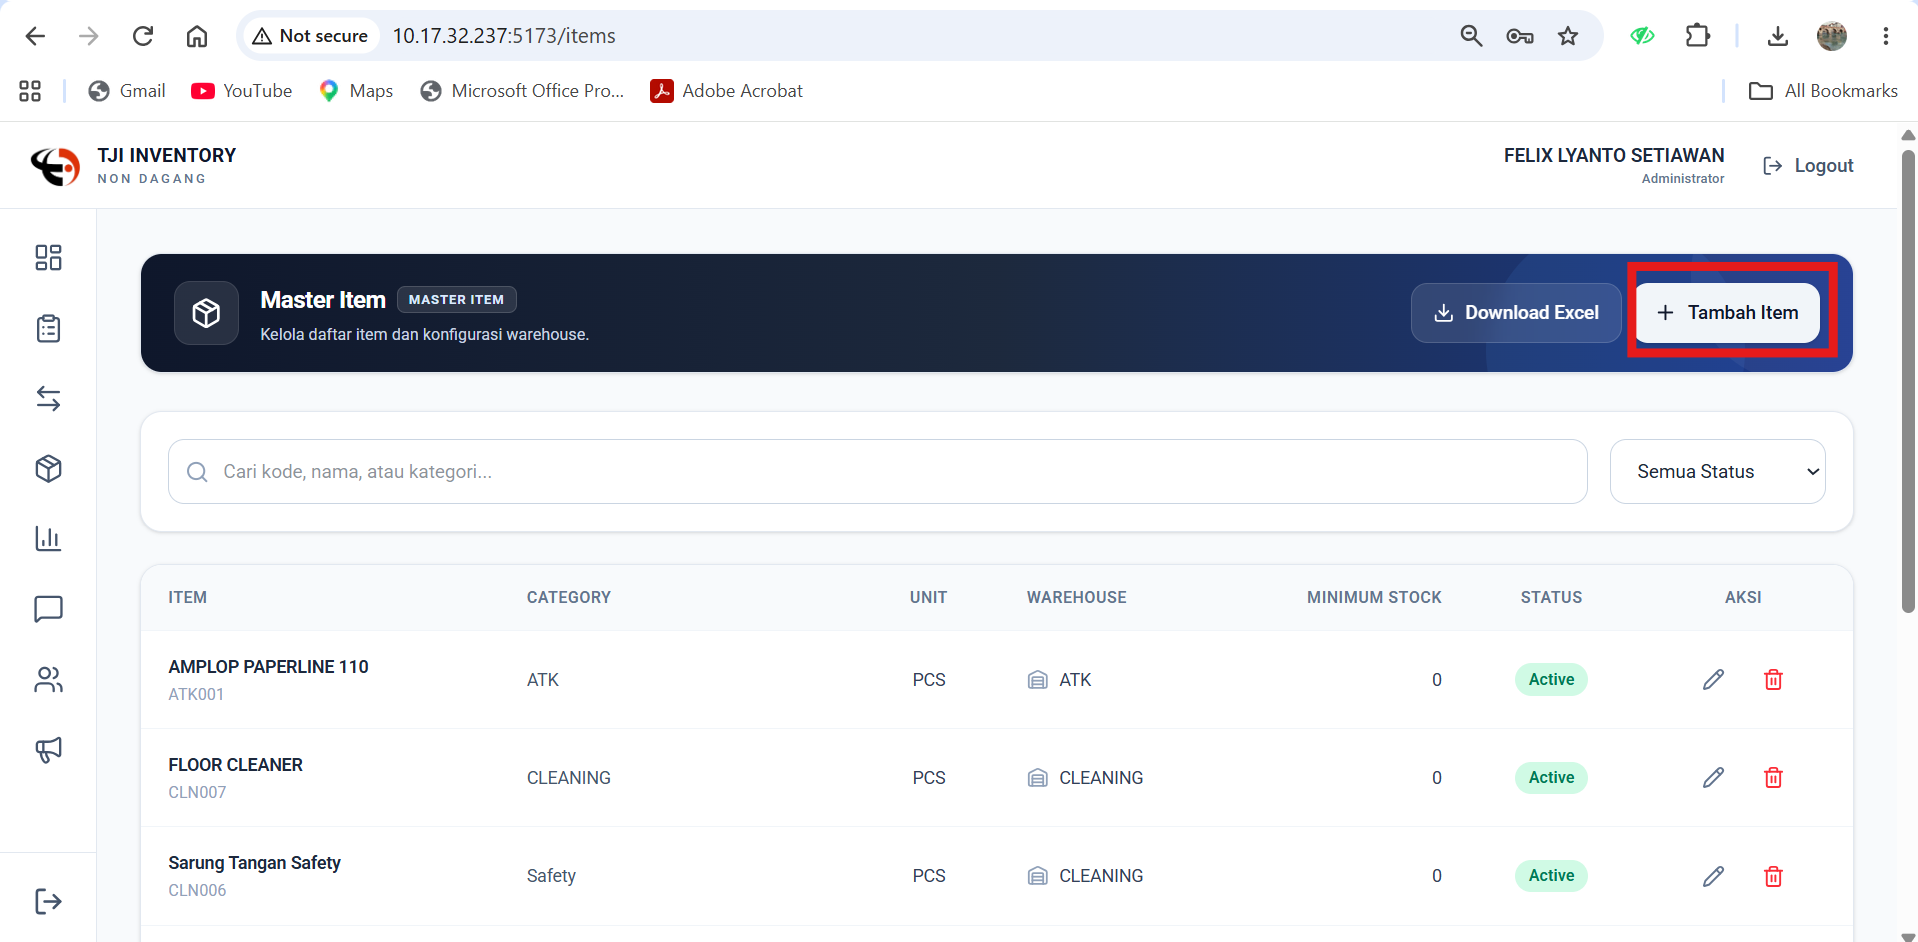
\includegraphics[
						width=0.95\linewidth,
						keepaspectratio
						]{images/Master Item/CreateItem2.png}
					}
					
					\only<3>{
						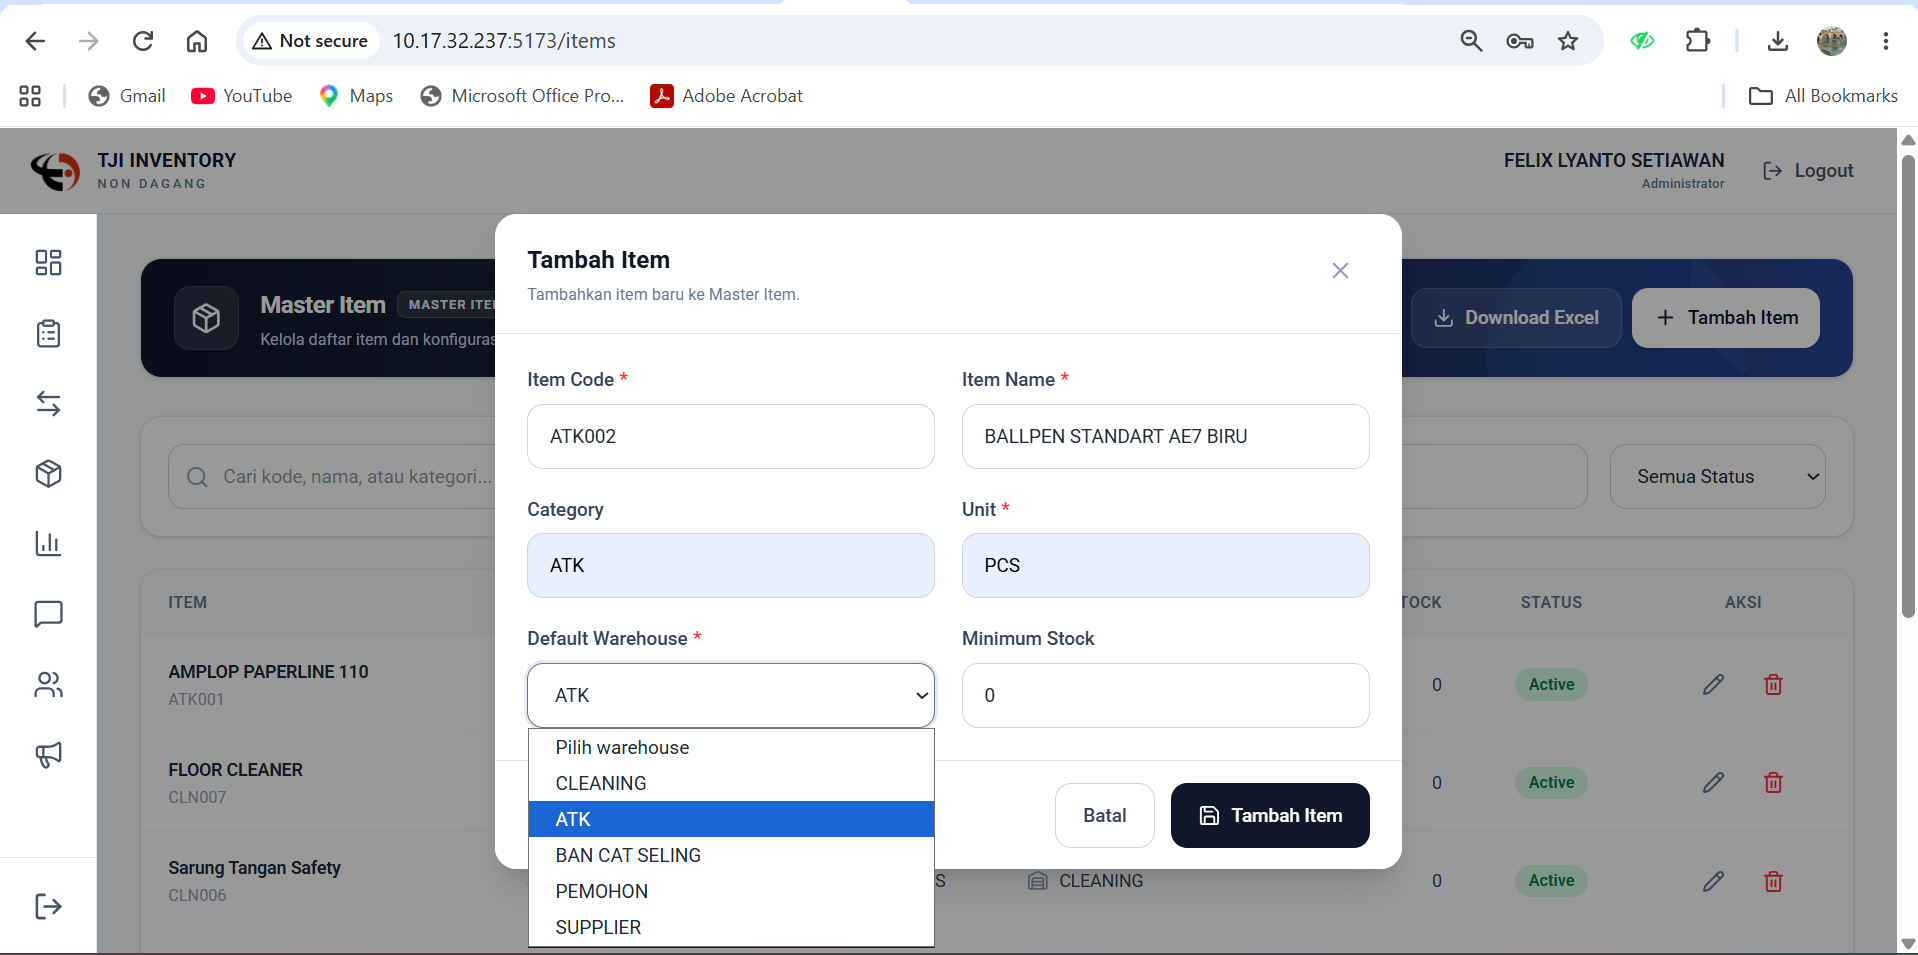
\includegraphics[
						width=0.95\linewidth,
						keepaspectratio
						]{images/Master Item/CreateItem3.png}
					}
					
					\only<4>{
						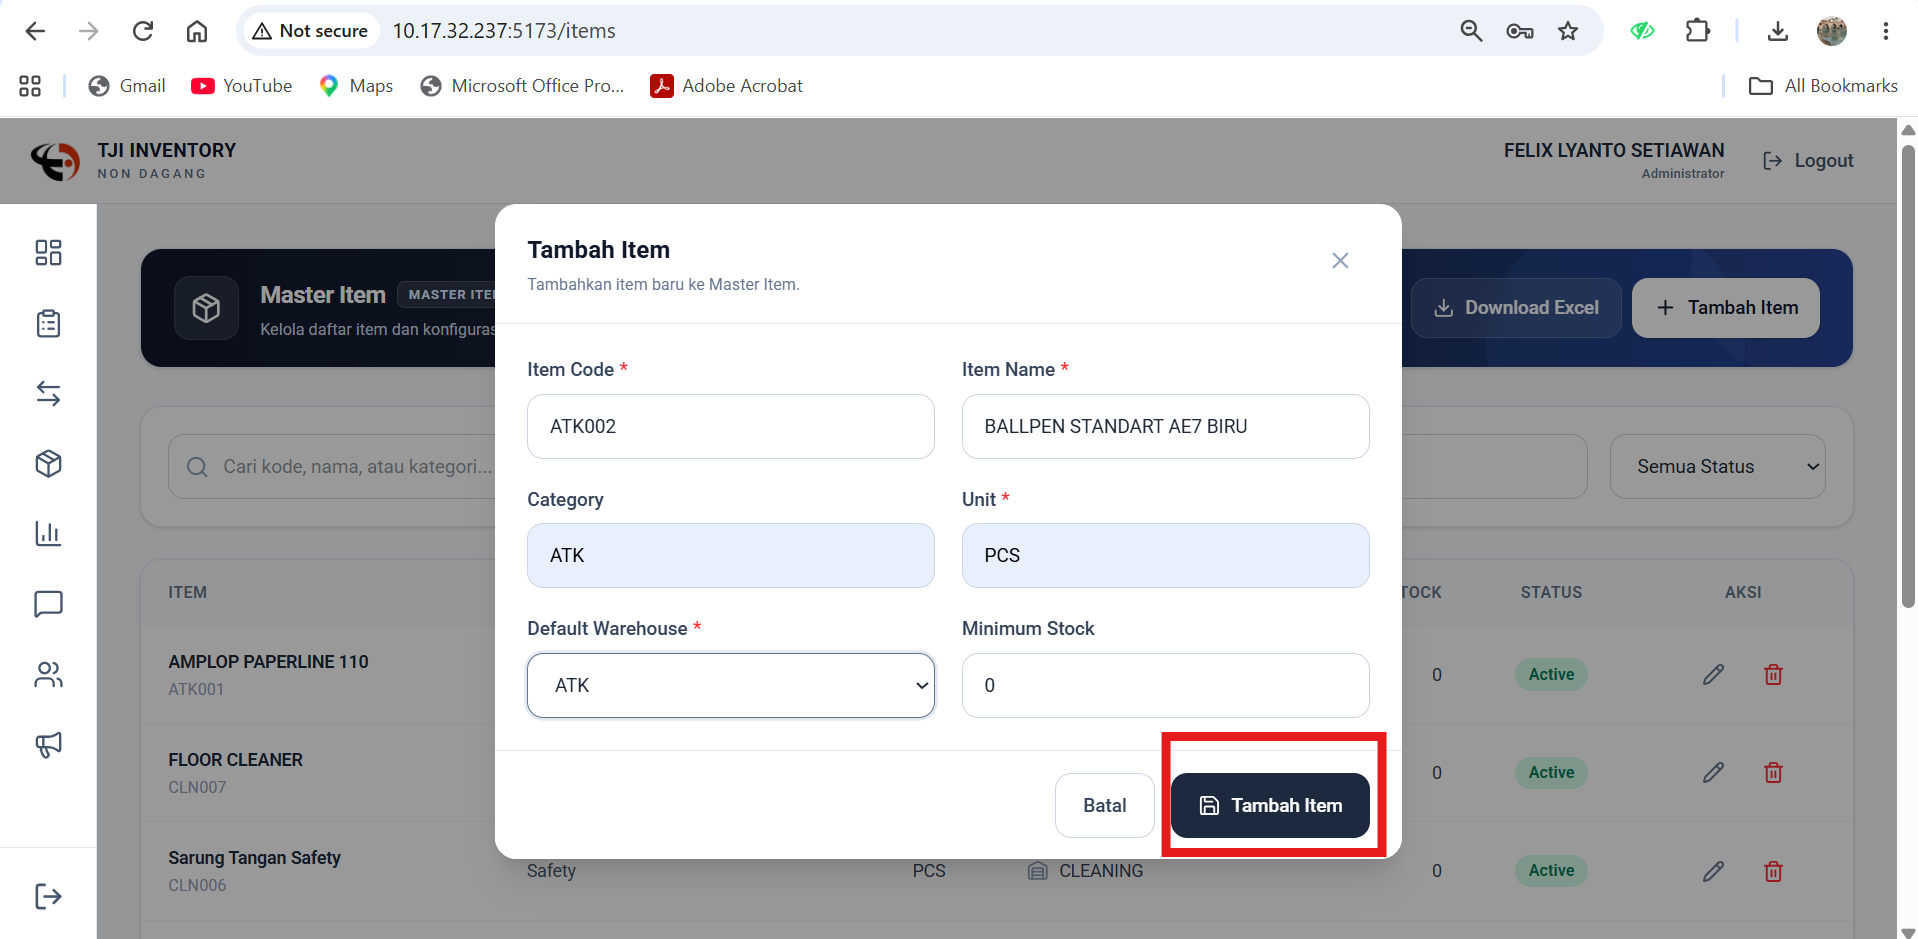
\includegraphics[
						width=0.95\linewidth,
						keepaspectratio
						]{images/Master Item/CreateItem4.png}
					}
					
					\only<5>{
						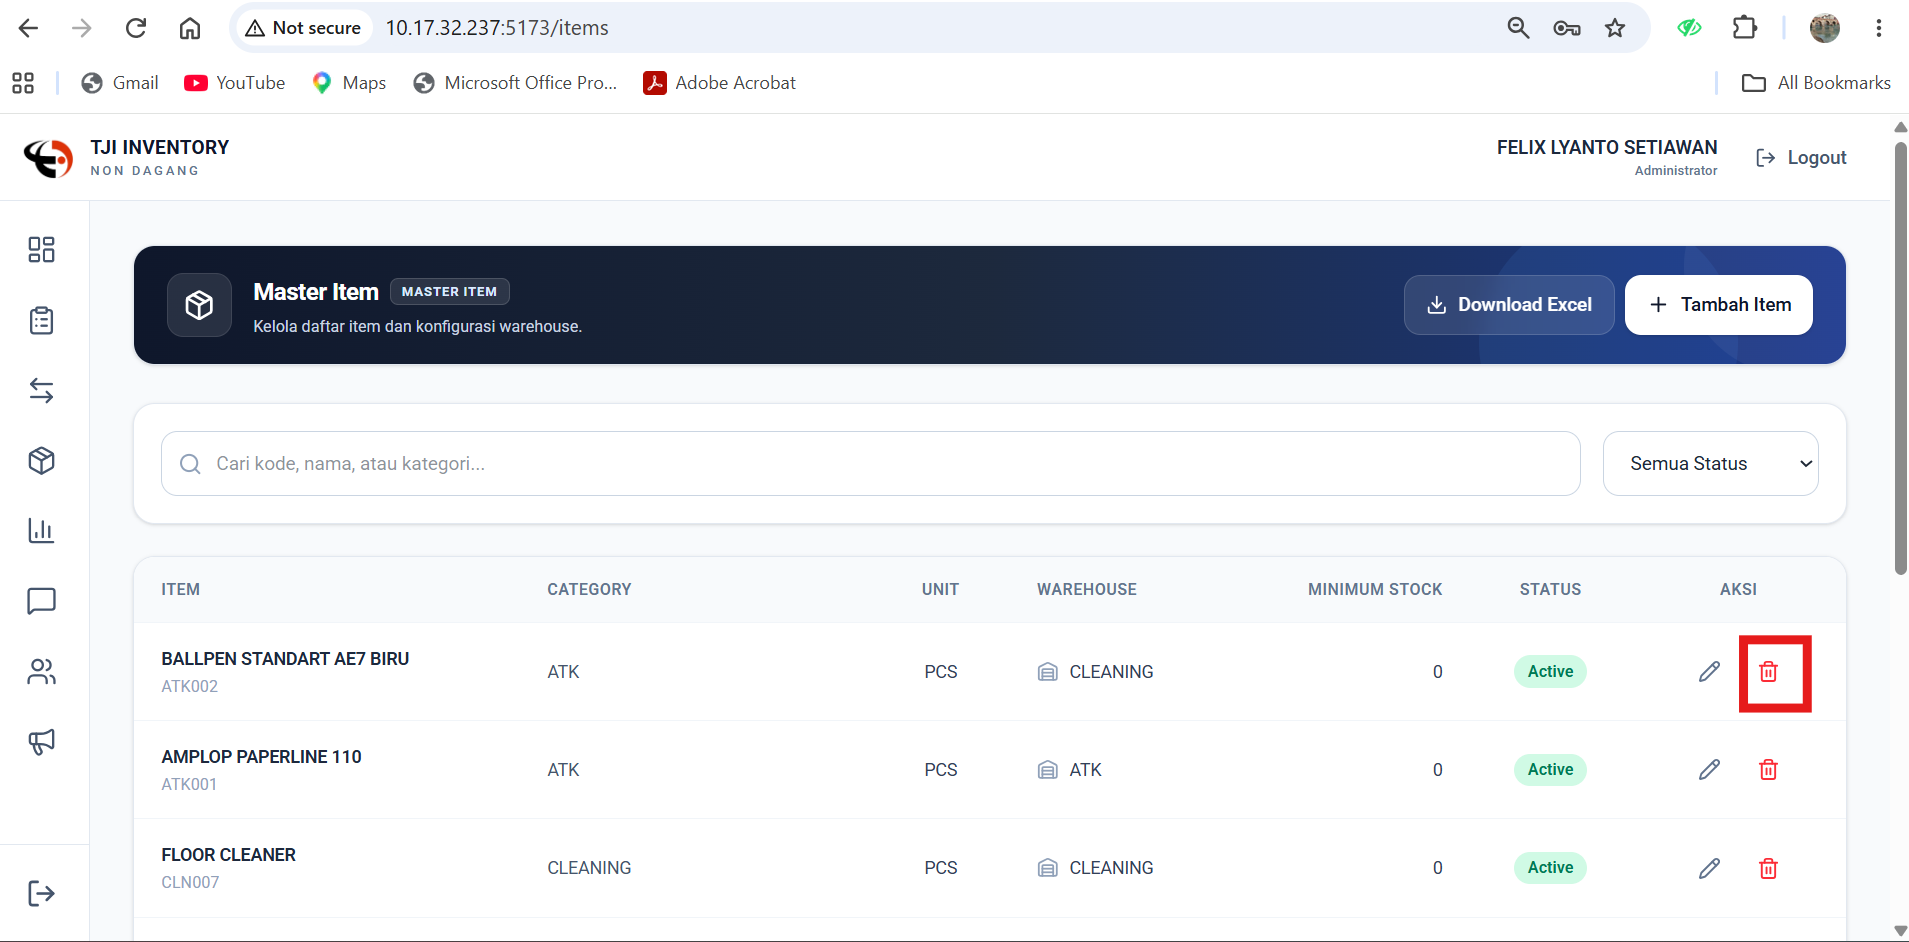
\includegraphics[
						width=0.95\linewidth,
						keepaspectratio
						]{images/Master Item/CreateItem5.png}
					}
					
					\only<6>{
						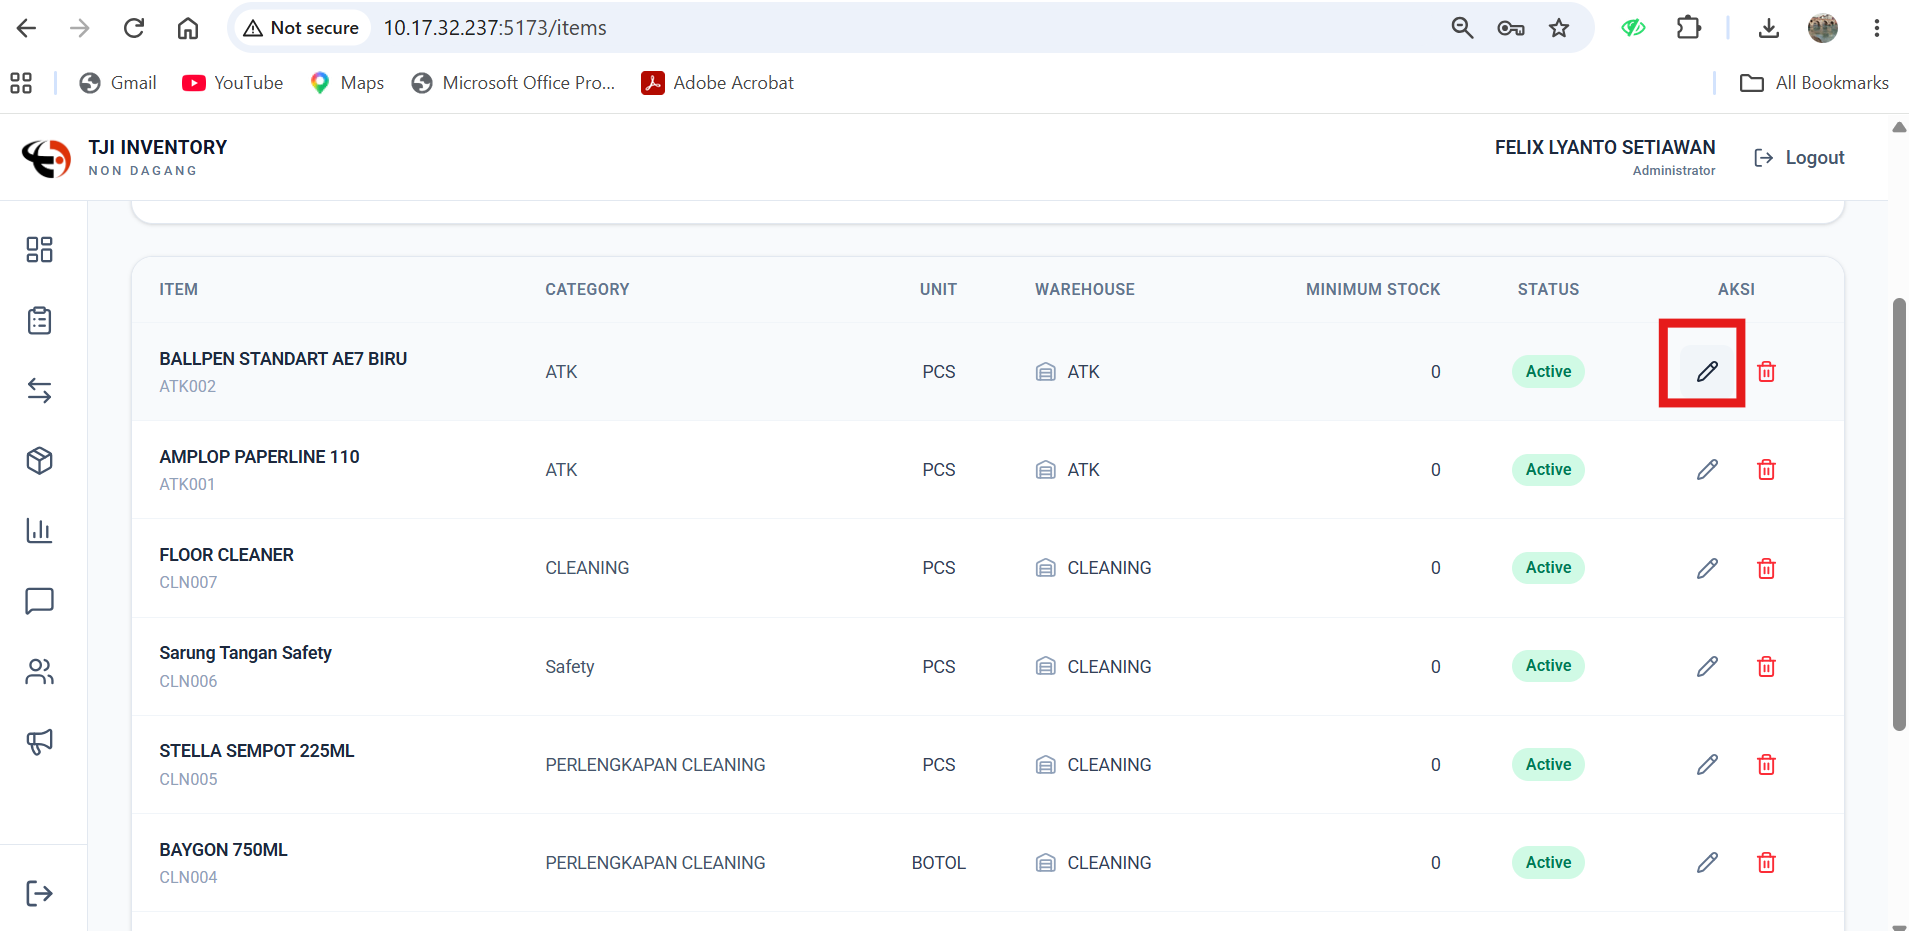
\includegraphics[
						width=0.95\linewidth,
						keepaspectratio
						]{images/Master Item/CreateItem6.png}
					}
					
					\only<7>{
						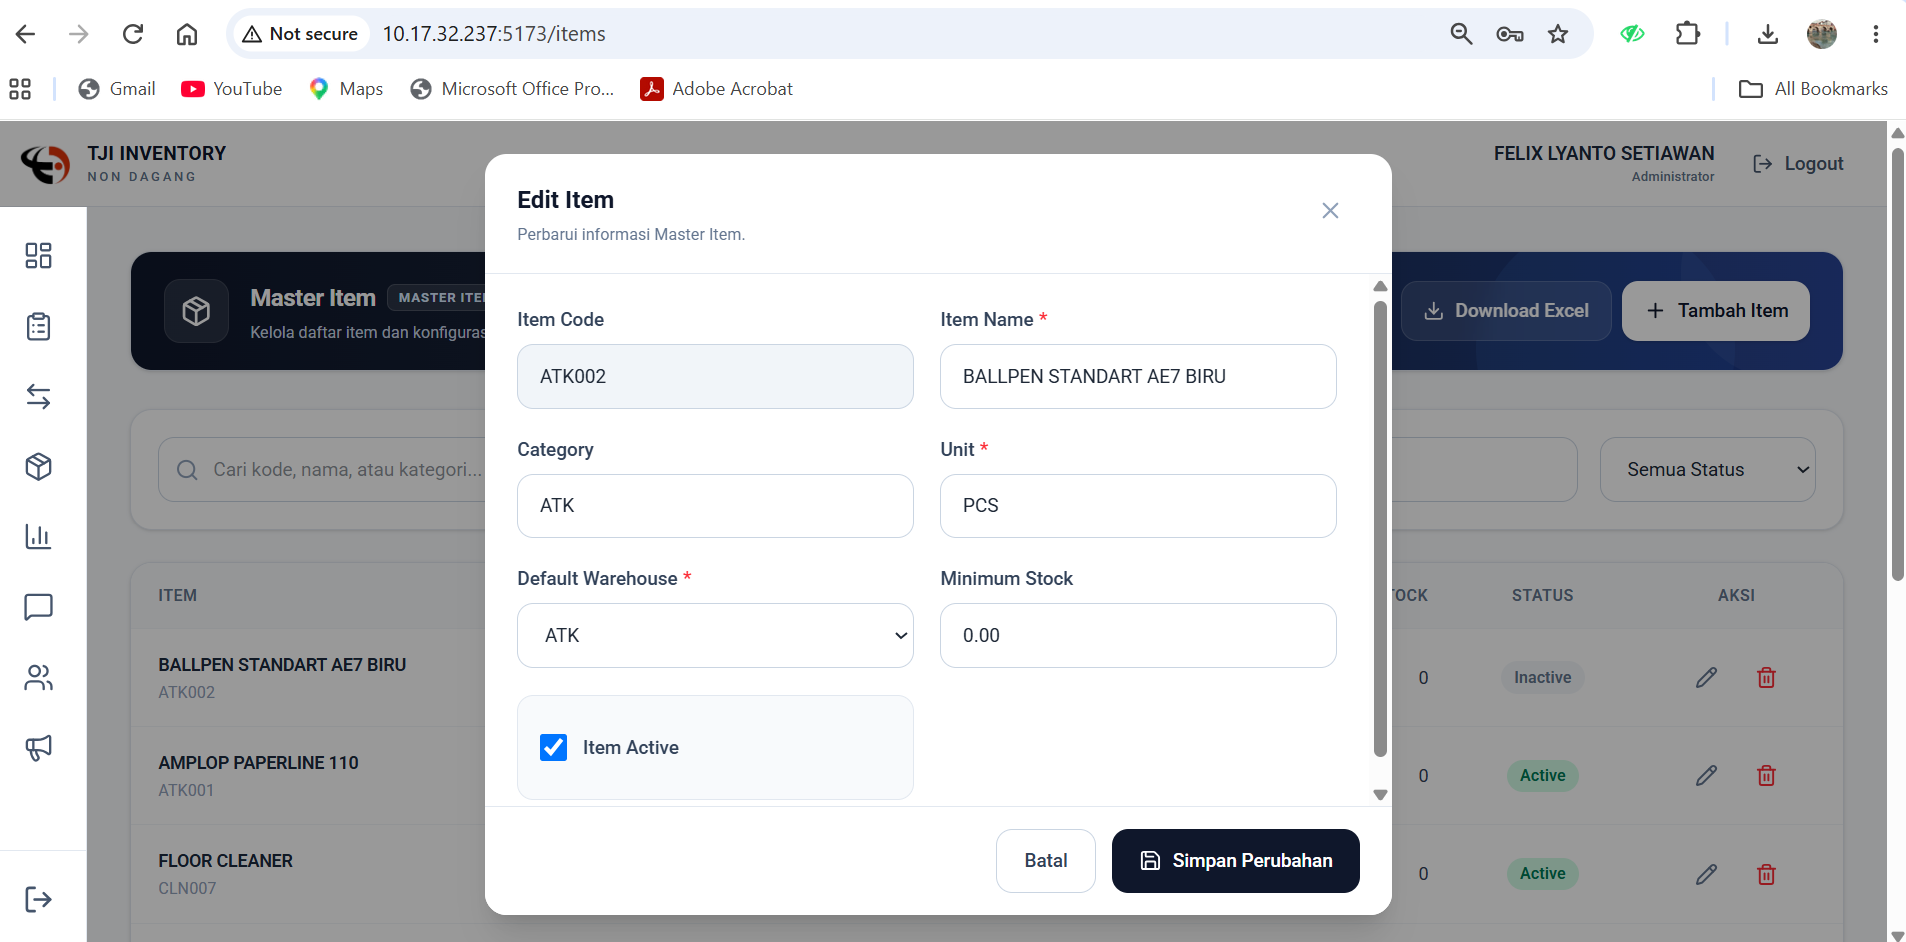
\includegraphics[
						width=0.95\linewidth,
						keepaspectratio
						]{images/Master Item/CreateItem7.png}
					}
					
					\only<8>{
						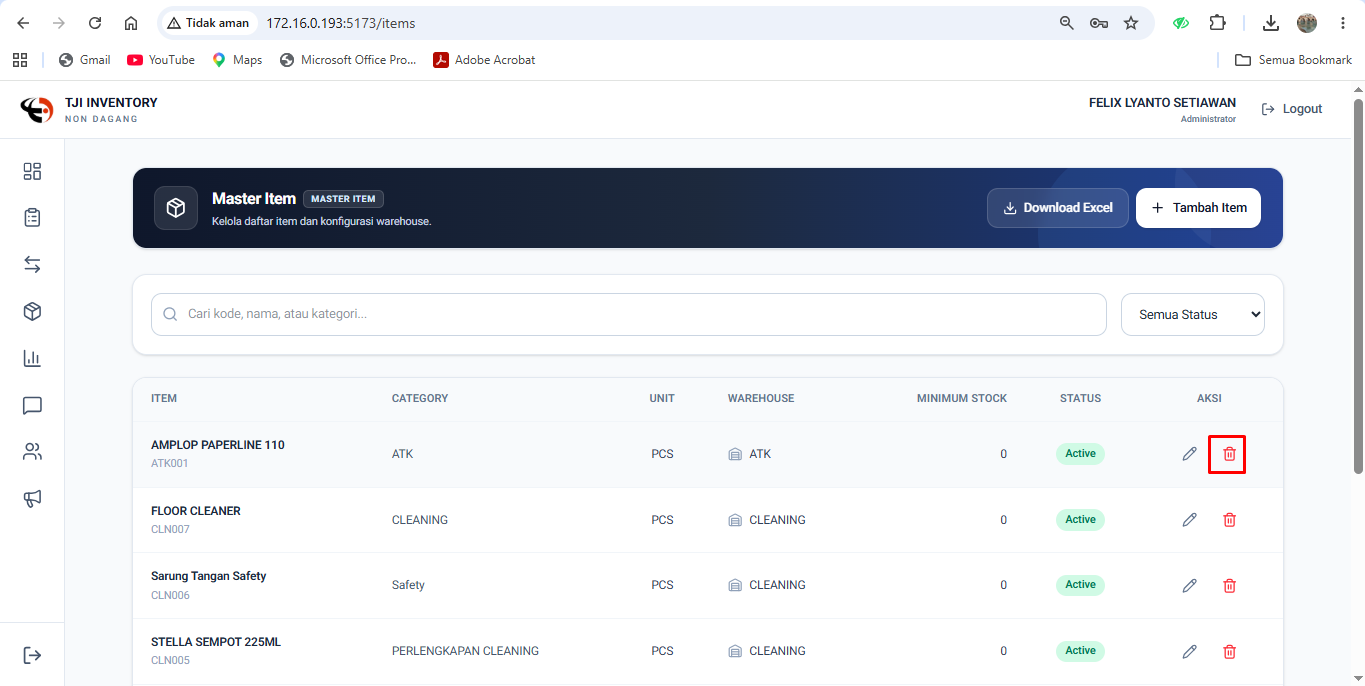
\includegraphics[
						width=0.95\linewidth,
						keepaspectratio
						]{images/Master Item/CreateItem8.png}
					}
				};
				
			\end{tikzpicture}
			
		\end{center}
		
		\column{0.025\textwidth}
		
		\column{0.325\textwidth}
		
		\stepcounterdisplay{1}{8}
		\stepcounterdisplay{2}{8}
		\stepcounterdisplay{3}{8}
		\stepcounterdisplay{4}{8}
		\stepcounterdisplay{5}{8}
		\stepcounterdisplay{6}{8}
		\stepcounterdisplay{7}{8}
		\stepcounterdisplay{8}{8}
		
		\sectionlabel{Langkah}
		
		\vspace{0.08cm}
		
		\stepitem{1}{1}{
			Pilih menu \textbf{Master Item}.
		}
		
		\vspace{\TutorialGap}
		
		\stepitem{2}{2}{
			Pilih \textbf{Tambah Item} untuk membuat
			item baru.
		}
		
		\vspace{\TutorialGap}
		
		\stepitem{3}{3}{
			Isikan informasi item sesuai dengan
			data barang yang akan dibuat.
		}
		
		\vspace{\TutorialGap}
		
		\stepitem{4}{4}{
			Apabila data item sudah lengkap dan benar \textbf{Pilih Tambah Item}
		}
		
		\vspace{\TutorialGap}
		
		\stepitem{5}{5}{
			Periksa kembali seluruh informasi item
			didalam list berikut sudah benar.
		}
		
		\vspace{\TutorialGap}
		
		\stepitem{6}{6}{
			Jika ada perbaikan ikon Pensil.
		}
		
		\vspace{\TutorialGap}
		
		\stepitem{7}{7}{
			Perbaiki informasi item yang belum tepat $>$ Pilih \textbf{Simpan Perubahan}
		}
		
		\vspace{\TutorialGap}
		
		\stepitem{8}{8}{
			Jika ingin menghapus item pilih ikon Tong Sampah.
		}

		
	\end{columns}
	
\end{frame}









%

% =========================================================
% REPORT
% =========================================================

\begin{frame}{06 --- Reports}
	
	\vfill
	
	\begin{center}
		
		\sectionlabel{Jenis-Jenis Report}
		
		\vspace{0.45cm}
		
		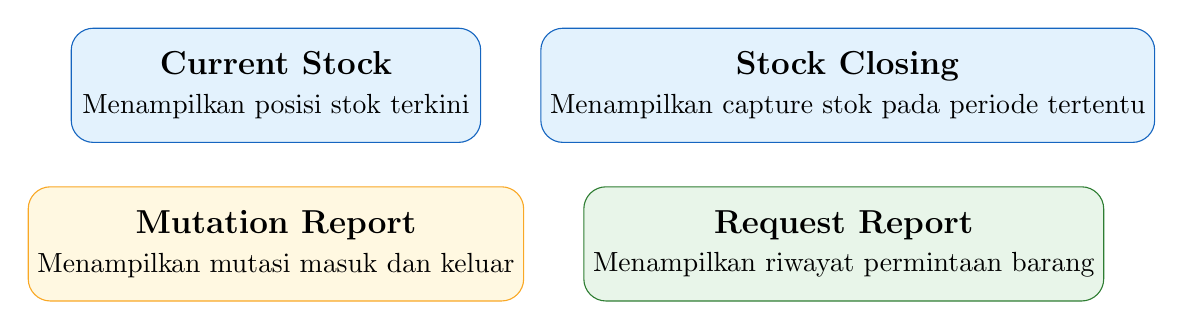
\begin{tikzpicture}[
			node distance=0.55cm and 0.75cm
			]
			
			% Current Stock
			\node[
			draw=Primary,
			fill=Secondary,
			rounded corners=8pt,
			minimum width=5.2cm,
			minimum height=1.45cm,
			align=center,
			font=\large
			]
			(current)
			{\textbf{Current Stock}\\
				\normalsize Menampilkan posisi stok terkini};
			
			% Stock Closing
			\node[
			draw=Primary,
			fill=Secondary,
			rounded corners=8pt,
			minimum width=5.2cm,
			minimum height=1.45cm,
			align=center,
			font=\large,
			right=of current
			]
			(closing)
			{\textbf{Stock Closing}\\
				\normalsize Menampilkan capture stok pada periode tertentu};
			
			% Mutation Report
			\node[
			draw=Warning,
			fill=WarningLight,
			rounded corners=8pt,
			minimum width=5.2cm,
			minimum height=1.45cm,
			align=center,
			font=\large,
			below=of current
			]
			(mutation)
			{\textbf{Mutation Report}\\
				\normalsize Menampilkan mutasi masuk dan keluar};
			
			% Request Report
			\node[
			draw=Success,
			fill=SuccessLight,
			rounded corners=8pt,
			minimum width=5.2cm,
			minimum height=1.45cm,
			align=center,
			font=\large,
			right=of mutation
			]
			(request)
			{\textbf{Request Report}\\
				\normalsize Menampilkan riwayat permintaan barang};
			
		\end{tikzpicture}
		
		\vspace{0.55cm}
		
		\infobox{Tujuan Report}{
			Report digunakan untuk memantau kondisi stok, pergerakan barang, serta riwayat permintaan secara terstruktur dan terdokumentasi, sehingga mempermudah seluruh pihak dalam melakukan monitoring, analisis, dan audit.

		}
		
	\end{center}
	
	\vfill
	
\end{frame}


\begin{frame}{06.1 --- Current Stock}
	
	\vspace{-0.15cm}
	
	\begin{columns}[T,totalwidth=\textwidth]
		
		% =========================
		% GAMBAR
		% =========================
		\column{0.62\textwidth}
		
		\begin{center}
			\begin{tikzpicture}
				\node[
				draw=LightGray,
				fill=white,
				rounded corners=8pt,
				inner sep=0.12cm
				] {
					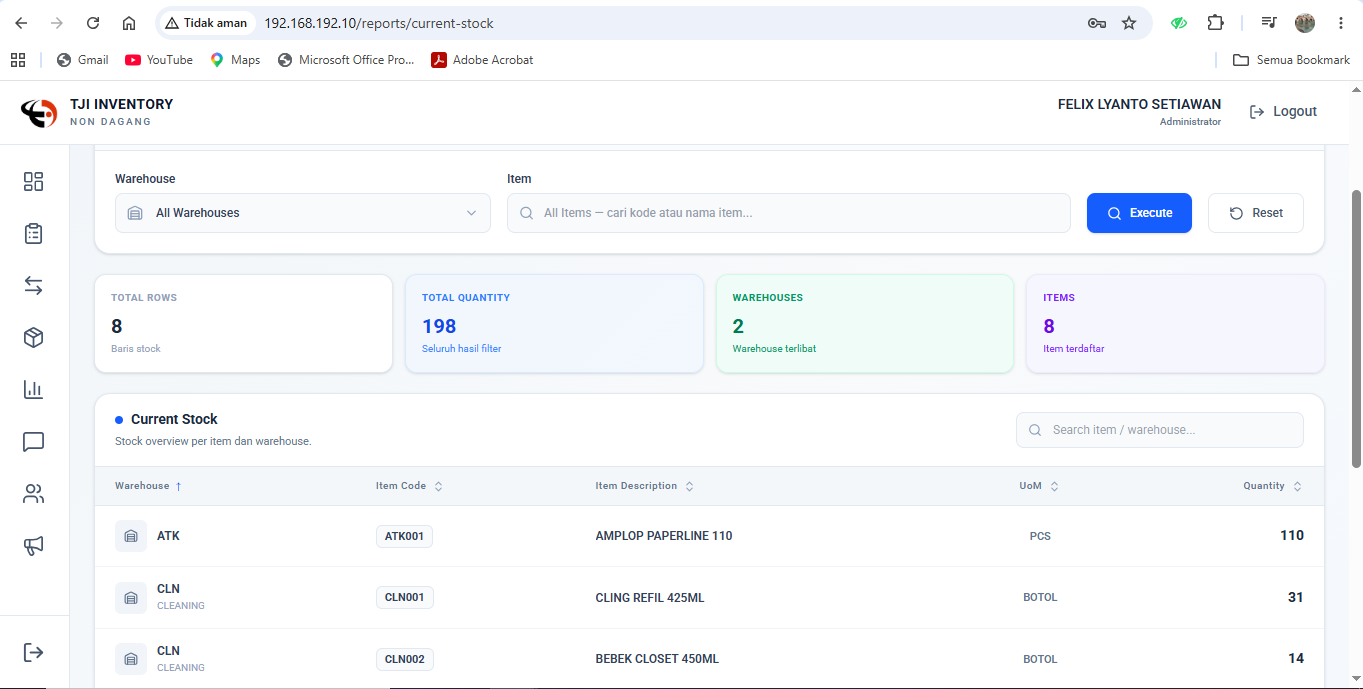
\includegraphics[
					width=0.96\linewidth,
					keepaspectratio
					]{images/Reports/CurrentStock.png}
				};
			\end{tikzpicture}
		\end{center}
		
		
		% =========================
		% KETERANGAN
		% =========================
		\column{0.04\textwidth}
		
		
		\column{0.34\textwidth}
		
		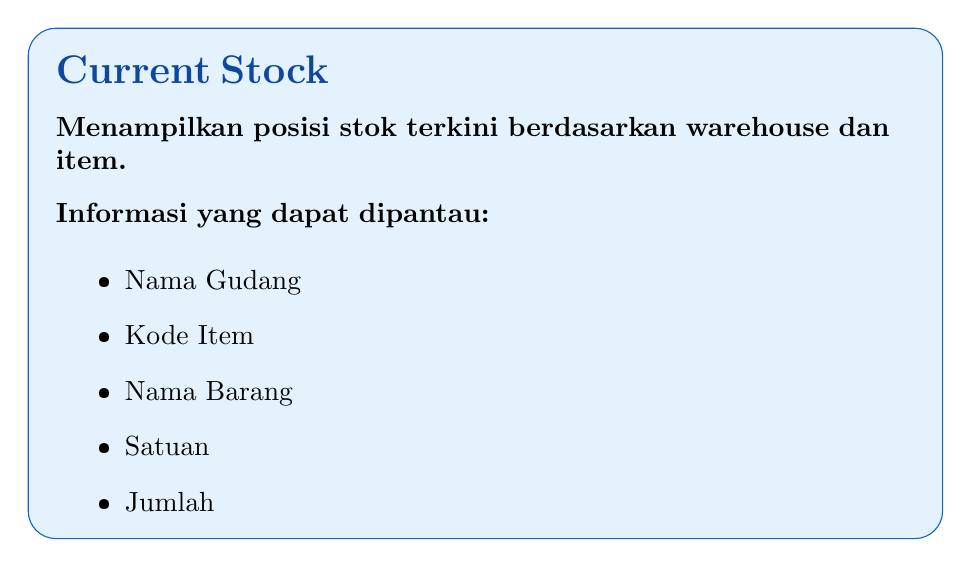
\begin{tikzpicture}
			\node[
			draw=Primary,
			fill=Secondary,
			rounded corners=10pt,
			inner sep=0.35cm,
			text width=0.90\linewidth,
			align=left
			] {
				{\Large\textbf{\textcolor{PrimaryDark}{Current Stock}}}
				
				\vspace{0.25cm}
				
				\normalsize
				\textbf{Menampilkan posisi stok terkini
				berdasarkan warehouse dan item.}
				
				\vspace{0.25cm}
				
				\textbf{Informasi yang dapat dipantau:}
				
				\vspace{0.08cm}
				
				\begin{itemize}
					\item Nama Gudang
					\item Kode Item
					\item Nama Barang
					\item Satuan
					\item Jumlah
				\end{itemize}
			};
		\end{tikzpicture}
		
	\end{columns}
	
\end{frame}


\begin{frame}{06.2 --- Stock Closing}
	
	\vspace{-0.15cm}
	
	\begin{columns}[T,totalwidth=\textwidth]
		
		% =========================
		% GAMBAR
		% =========================
		\column{0.62\textwidth}
		
		\begin{center}
			\begin{tikzpicture}
				\node[
				draw=LightGray,
				fill=white,
				rounded corners=8pt,
				inner sep=0.12cm
				] {
					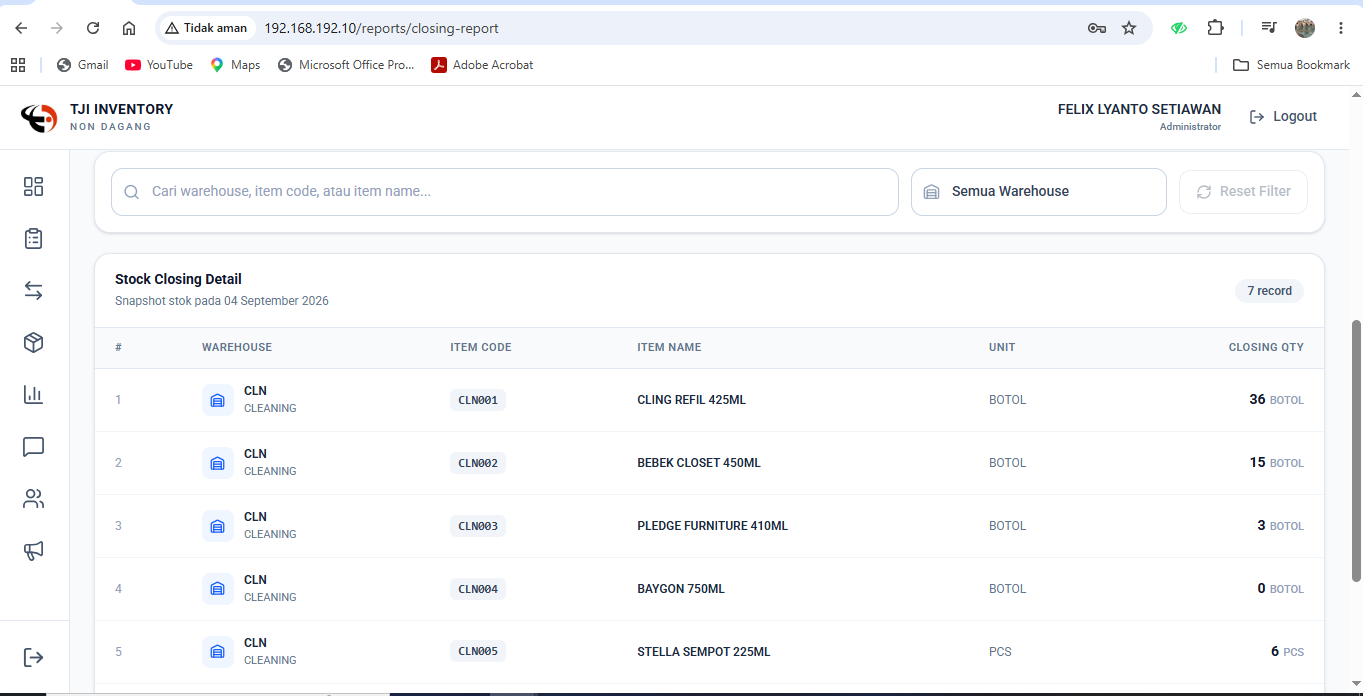
\includegraphics[
					width=0.96\linewidth,
					keepaspectratio
					]{images/Reports/StockClosing.png}
				};
			\end{tikzpicture}
		\end{center}
		
		
		% =========================
		% JARAK
		% =========================
		\column{0.04\textwidth}
		
		
		% =========================
		% KETERANGAN
		% =========================
		\column{0.34\textwidth}
		
		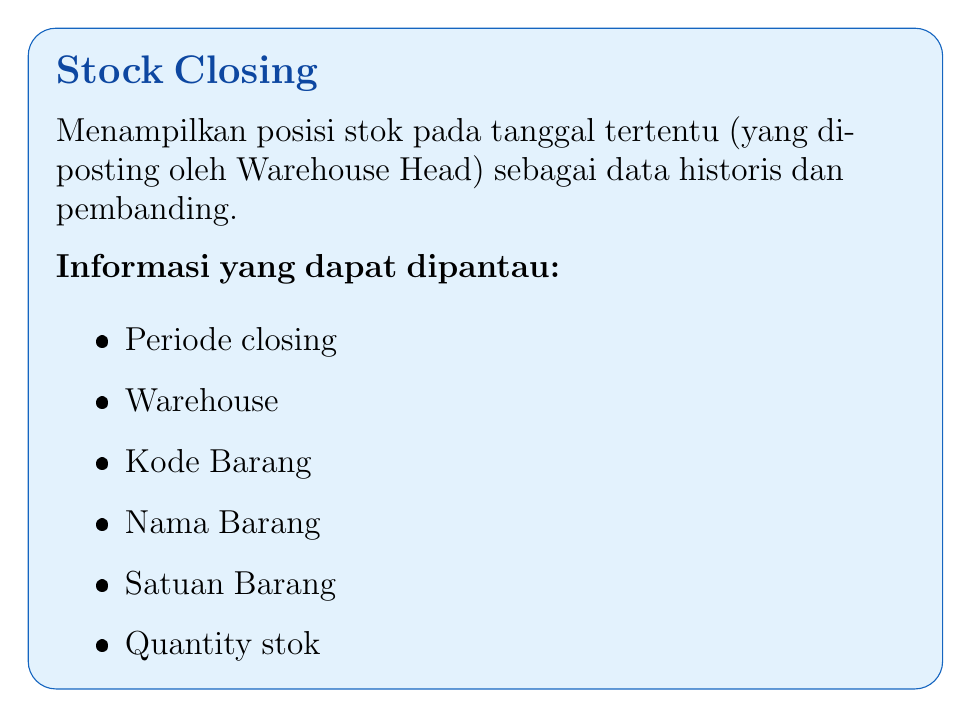
\begin{tikzpicture}
			\node[
			draw=Primary,
			fill=Secondary,
			rounded corners=10pt,
			inner sep=0.35cm,
			text width=0.90\linewidth,
			align=left
			] {
				{\Large\textbf{\textcolor{PrimaryDark}{Stock Closing}}}
				
				\vspace{0.25cm}
				
				\large
				Menampilkan posisi stok pada
				tanggal tertentu (yang diposting oleh Warehouse Head) sebagai data
				historis dan pembanding.
				
				\vspace{0.25cm}
				
				\large\textbf{Informasi yang dapat dipantau:}
				
				\vspace{0.08cm}
				
				\large
				\begin{itemize}
					\item Periode closing
					\item Warehouse
					\item Kode Barang
					\item Nama Barang
					\item Satuan Barang
					\item Quantity stok
				\end{itemize}
			};
		\end{tikzpicture}
		
	\end{columns}
	
\end{frame}


\begin{frame}{06.3 --- Mutation Report}
	
	\vspace{-0.15cm}
	
	\begin{columns}[T,totalwidth=\textwidth]
		
		% =========================
		% GAMBAR
		% =========================
		\column{0.62\textwidth}
		
		\begin{center}
			\begin{tikzpicture}
				\node[
				draw=LightGray,
				fill=white,
				rounded corners=8pt,
				inner sep=0.12cm
				] {
					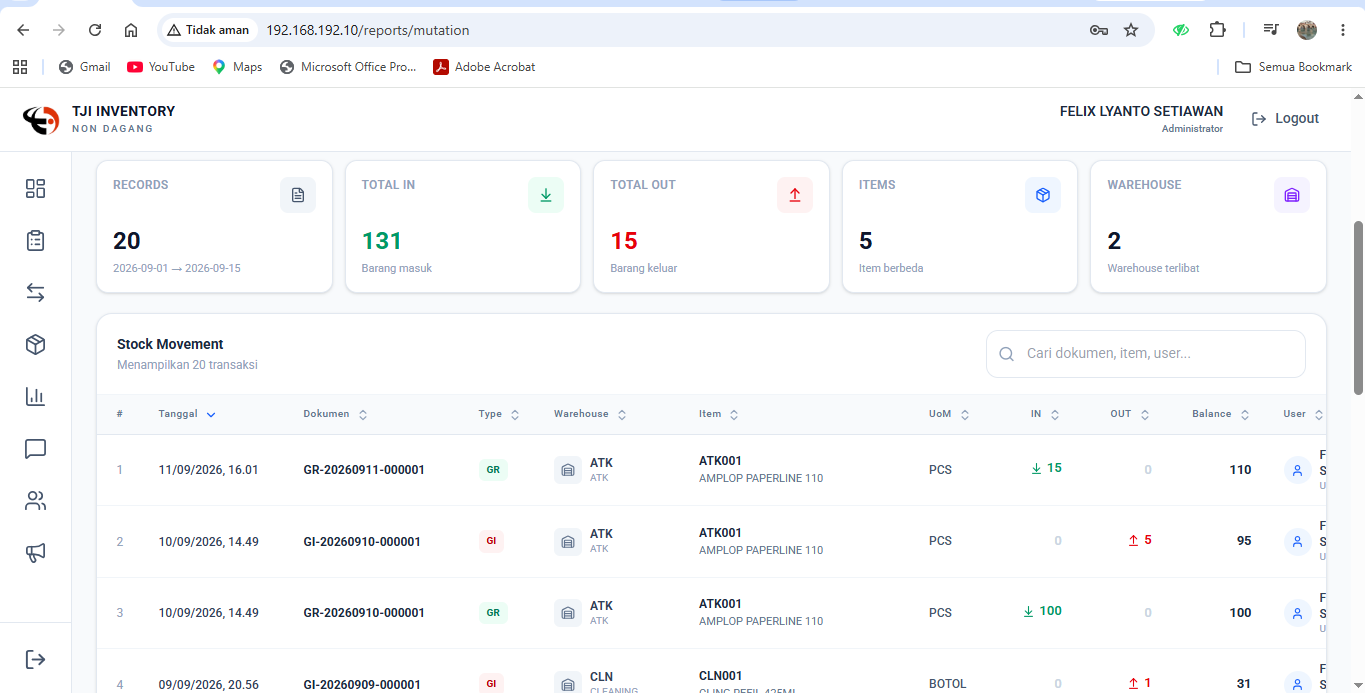
\includegraphics[
					width=0.96\linewidth,
					keepaspectratio
					]{images/Reports/MutationReport.png}
				};
			\end{tikzpicture}
		\end{center}
		
		
		% =========================
		% JARAK
		% =========================
		\column{0.04\textwidth}
		
		
		% =========================
		% KETERANGAN
		% =========================
		\column{0.34\textwidth}
		
		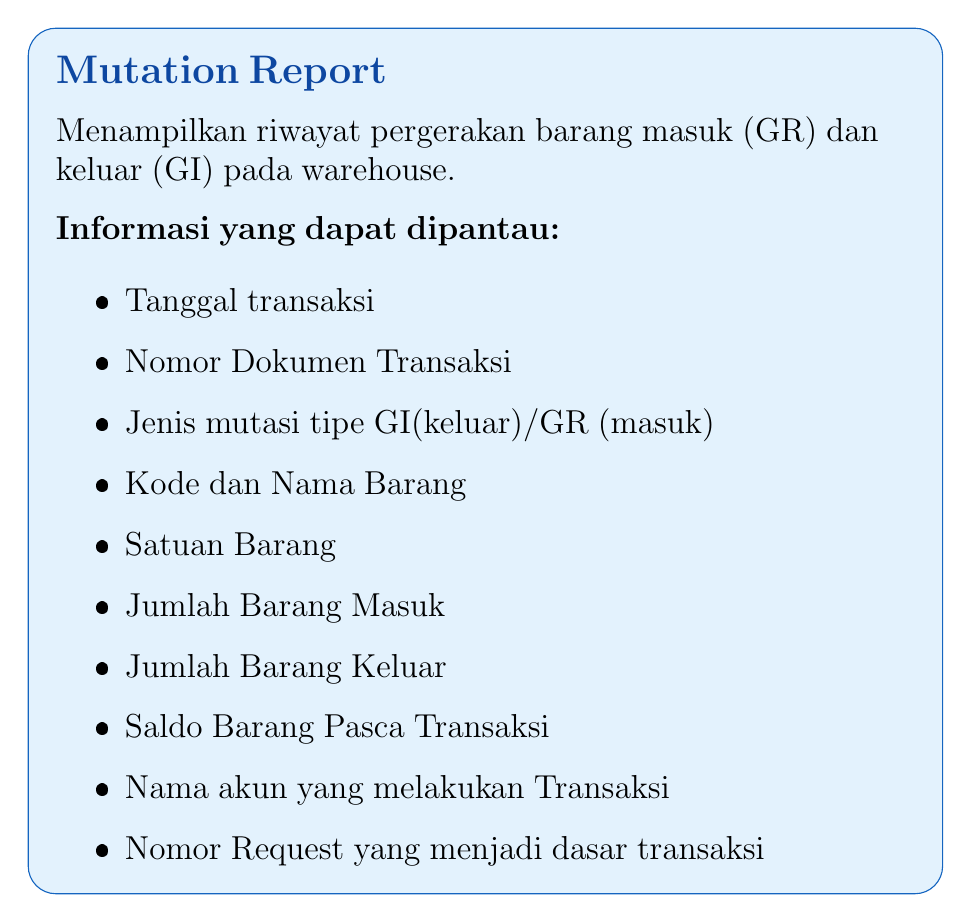
\begin{tikzpicture}
			\node[
			draw=Primary,
			fill=Secondary,
			rounded corners=10pt,
			inner sep=0.35cm,
			text width=0.90\linewidth,
			align=left
			] {
				{\Large\textbf{\textcolor{PrimaryDark}{Mutation Report}}}
				
				\vspace{0.25cm}
				
				\large
				Menampilkan riwayat pergerakan
				barang masuk (GR) dan keluar (GI)
				pada warehouse.
				
				\vspace{0.25cm}
				
				\large\textbf{Informasi yang dapat dipantau:}
				
				\vspace{0.08cm}
				
				\large
				\begin{itemize}
					\item Tanggal transaksi
					\item Nomor Dokumen Transaksi
					\item Jenis mutasi tipe GI(keluar)/GR (masuk)
					\item Kode dan Nama Barang
					\item Satuan Barang
					\item Jumlah Barang Masuk
					\item Jumlah Barang Keluar
					\item Saldo Barang Pasca Transaksi
					\item Nama akun yang melakukan Transaksi
					\item Nomor Request yang menjadi dasar transaksi
				\end{itemize}
			};
		\end{tikzpicture}
		
	\end{columns}
	
\end{frame}

\begin{frame}{06.4 --- Histori Request}
	
	\vspace{-0.15cm}
	
	\begin{columns}[T,totalwidth=\textwidth]
		
		% =========================
		% GAMBAR
		% =========================
		\column{0.62\textwidth}
		
		\begin{center}
			\begin{tikzpicture}
				\node[
				draw=LightGray,
				fill=white,
				rounded corners=8pt,
				inner sep=0.12cm
				] {
					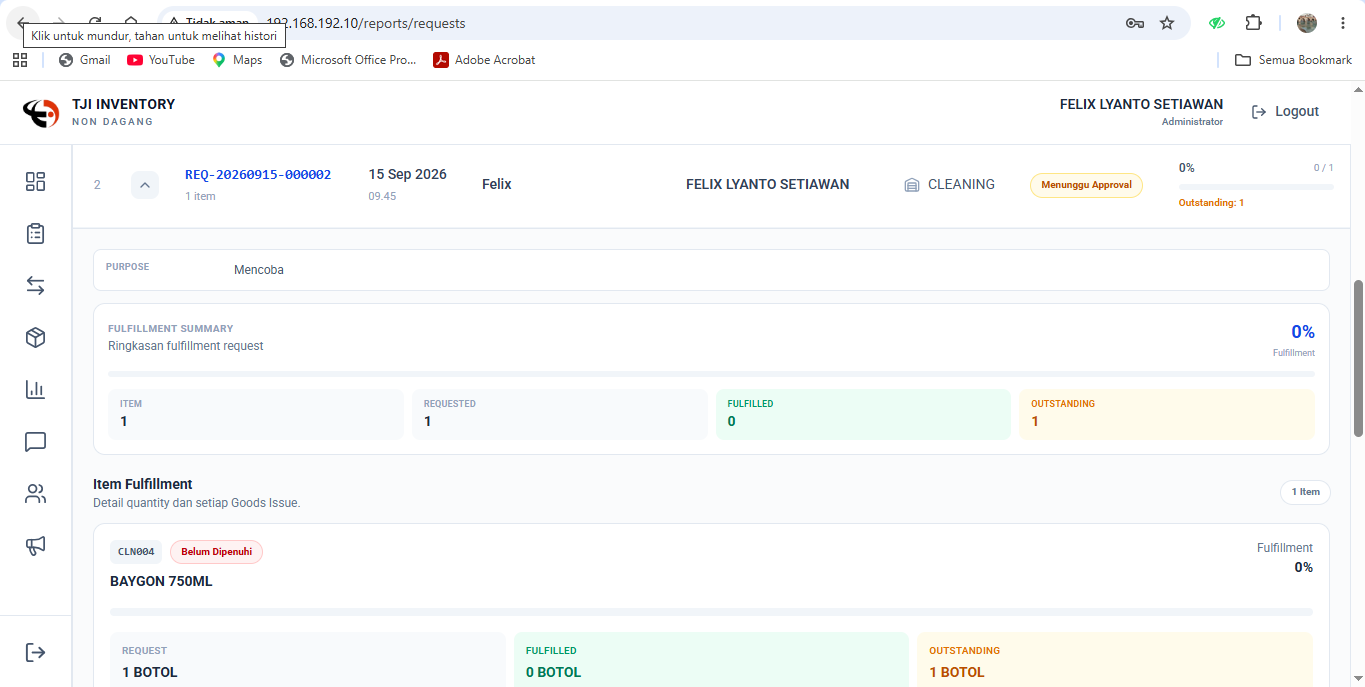
\includegraphics[
					width=0.96\linewidth,
					keepaspectratio
					]{images/Reports/RequestReport.png}
				};
			\end{tikzpicture}
		\end{center}
		
		
		% =========================
		% JARAK
		% =========================
		\column{0.04\textwidth}
		
		
		% =========================
		% KETERANGAN
		% =========================
		\column{0.34\textwidth}
		
		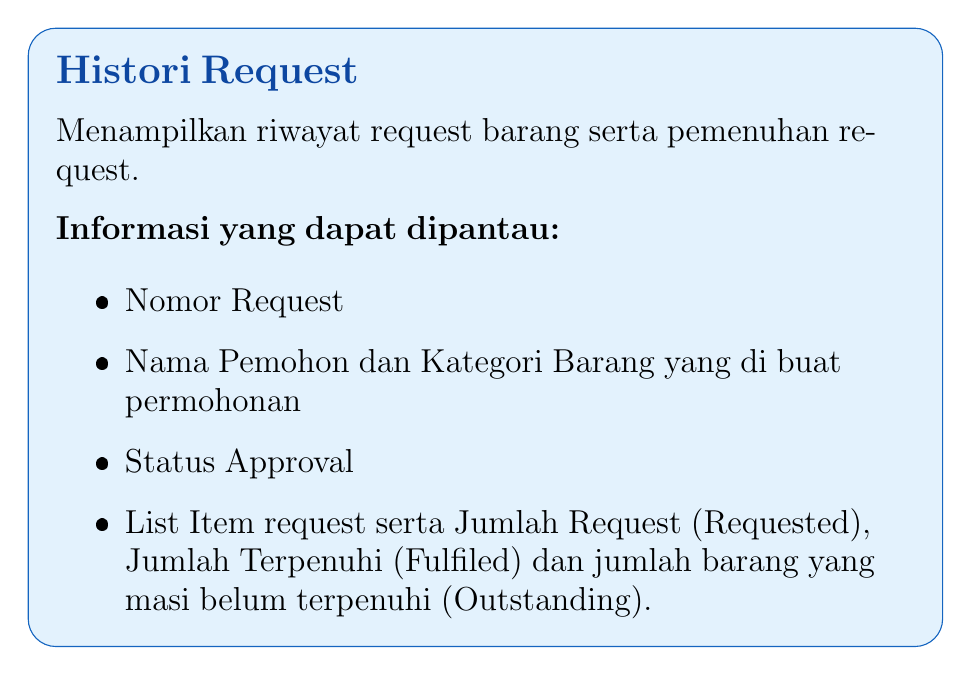
\begin{tikzpicture}
			\node[
			draw=Primary,
			fill=Secondary,
			rounded corners=10pt,
			inner sep=0.35cm,
			text width=0.90\linewidth,
			align=left
			] {
				{\Large\textbf{\textcolor{PrimaryDark}{Histori Request}}}
				
				\vspace{0.25cm}
				
				\large
				Menampilkan riwayat request barang
				serta pemenuhan request.
				
				\vspace{0.25cm}
				
				\large\textbf{Informasi yang dapat dipantau:}
				
				\vspace{0.08cm}
				
				\large
				\begin{itemize}
					\item Nomor Request
					\item Nama Pemohon dan Kategori Barang yang di buat permohonan
					\item Status Approval
					\item List Item request serta Jumlah Request (Requested), Jumlah Terpenuhi (Fulfiled) dan jumlah barang yang masi belum terpenuhi (Outstanding).
				\end{itemize}
			};
		\end{tikzpicture}
		
	\end{columns}
	
\end{frame}

\begin{frame}{07 --- Discussion}
	
	\vspace{-0.15cm}
	
	\begin{columns}[T,totalwidth=\textwidth]
		
		% =========================
		% GAMBAR
		% =========================
		\column{0.62\textwidth}
		
		\begin{center}
			\begin{tikzpicture}
				\node[
				draw=LightGray,
				fill=white,
				rounded corners=8pt,
				inner sep=0.12cm
				] {
					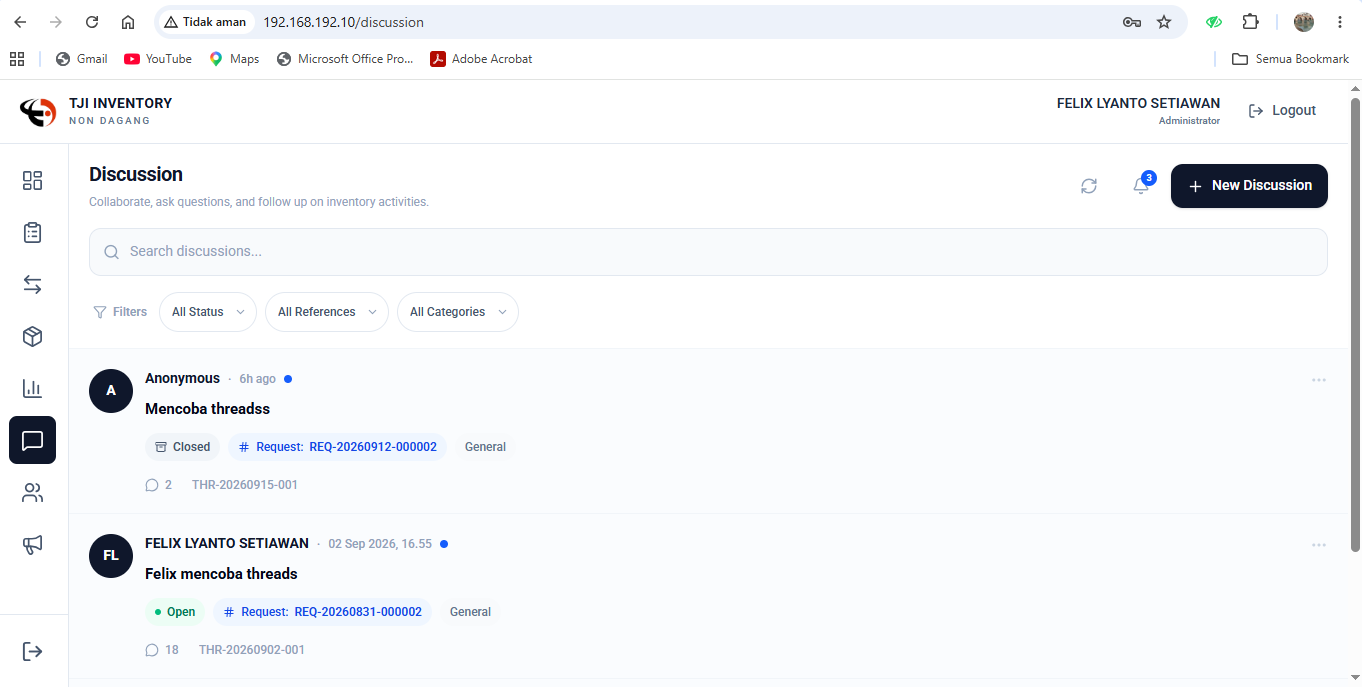
\includegraphics[
					width=0.96\linewidth,
					keepaspectratio
					]{images/Discussion/Discussion1.png}
				};
			\end{tikzpicture}
		\end{center}
		
		
		% =========================
		% JARAK
		% =========================
		\column{0.04\textwidth}
		
		
		% =========================
		% KETERANGAN
		% =========================
		\column{0.34\textwidth}
		
		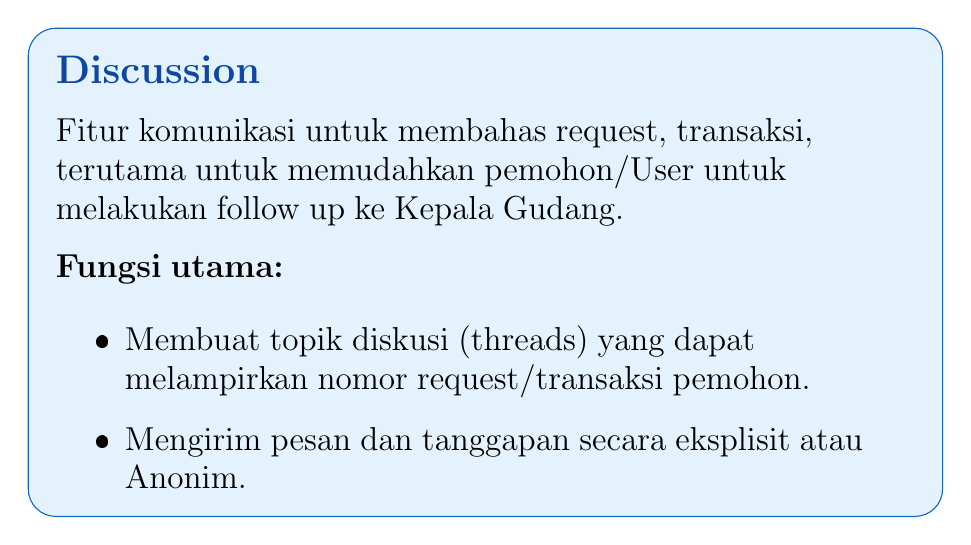
\begin{tikzpicture}
			\node[
			draw=Primary,
			fill=Secondary,
			rounded corners=10pt,
			inner sep=0.35cm,
			text width=0.90\linewidth,
			align=left
			] {
				{\Large\textbf{\textcolor{PrimaryDark}{Discussion}}}
				
				\vspace{0.25cm}
				
				\large
				Fitur komunikasi  untuk membahas
				request, transaksi, terutama untuk memudahkan pemohon/User untuk melakukan follow up ke Kepala Gudang.
				
				\vspace{0.25cm}
				
				\large\textbf{Fungsi utama:}
				
				\vspace{0.08cm}
				
				\large
				\begin{itemize}
					\item Membuat topik diskusi (threads) yang dapat melampirkan nomor request/transaksi pemohon.
					\item Mengirim pesan dan tanggapan secara eksplisit atau Anonim.
				\end{itemize}
			};
		\end{tikzpicture}
		
	\end{columns}
	
\end{frame}



\begin{frame}{07 --- Discussion}
	
	\vspace{-0.25cm}
	
	\begin{columns}[T,totalwidth=\textwidth]
		
		\column{0.65\textwidth}
		
		\begin{center}
			
			\begin{tikzpicture}
				
				\node[
				inner sep=0,
				outer sep=0
				] (screen)
				{
					\only<1>{
						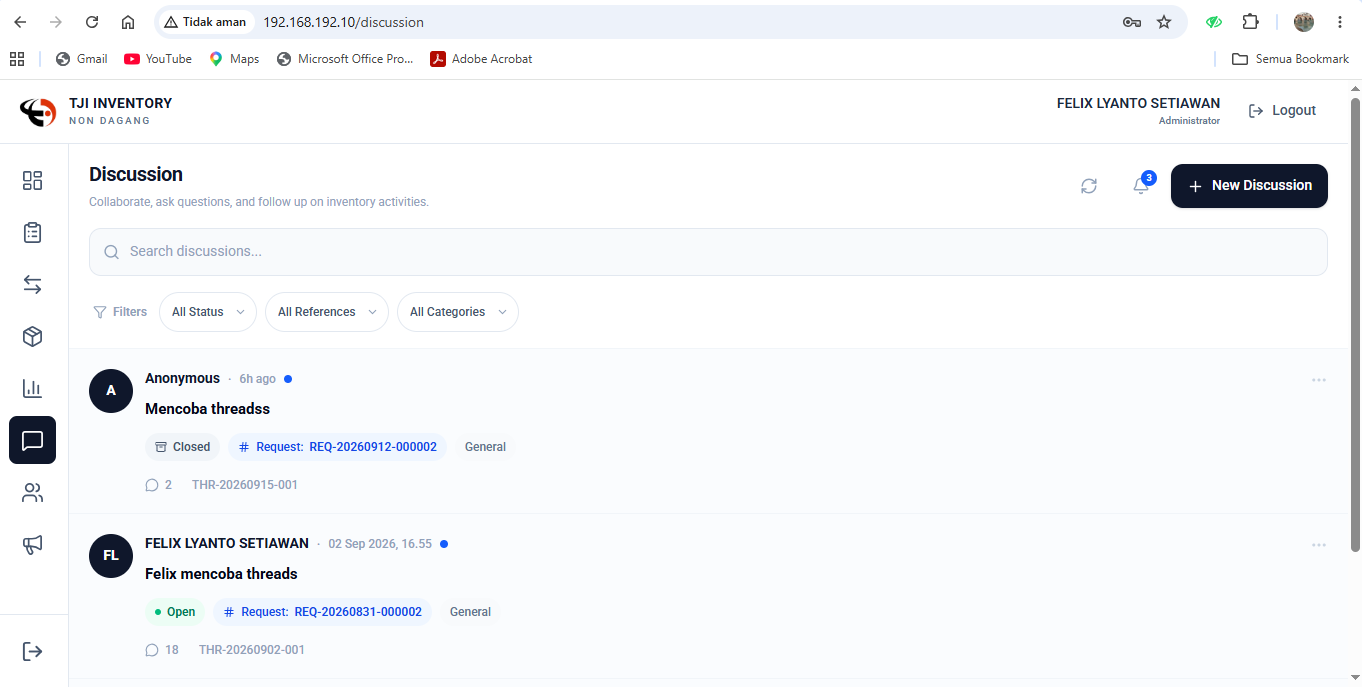
\includegraphics[
						width=0.95\linewidth,
						keepaspectratio
						]{images/Discussion/Discussion1.png}
					}
					
					\only<2>{
						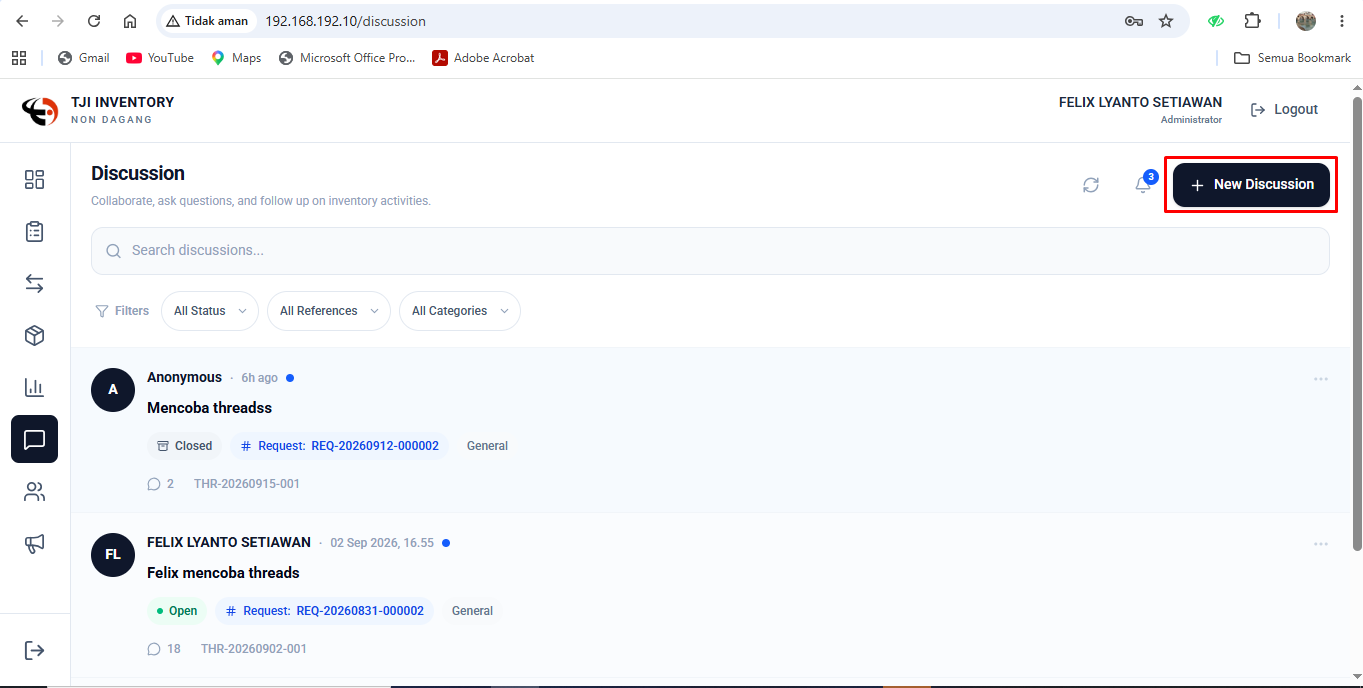
\includegraphics[
						width=0.95\linewidth,
						keepaspectratio
						]{images/Discussion/Discussion2.png}
					}
					
					\only<3>{
						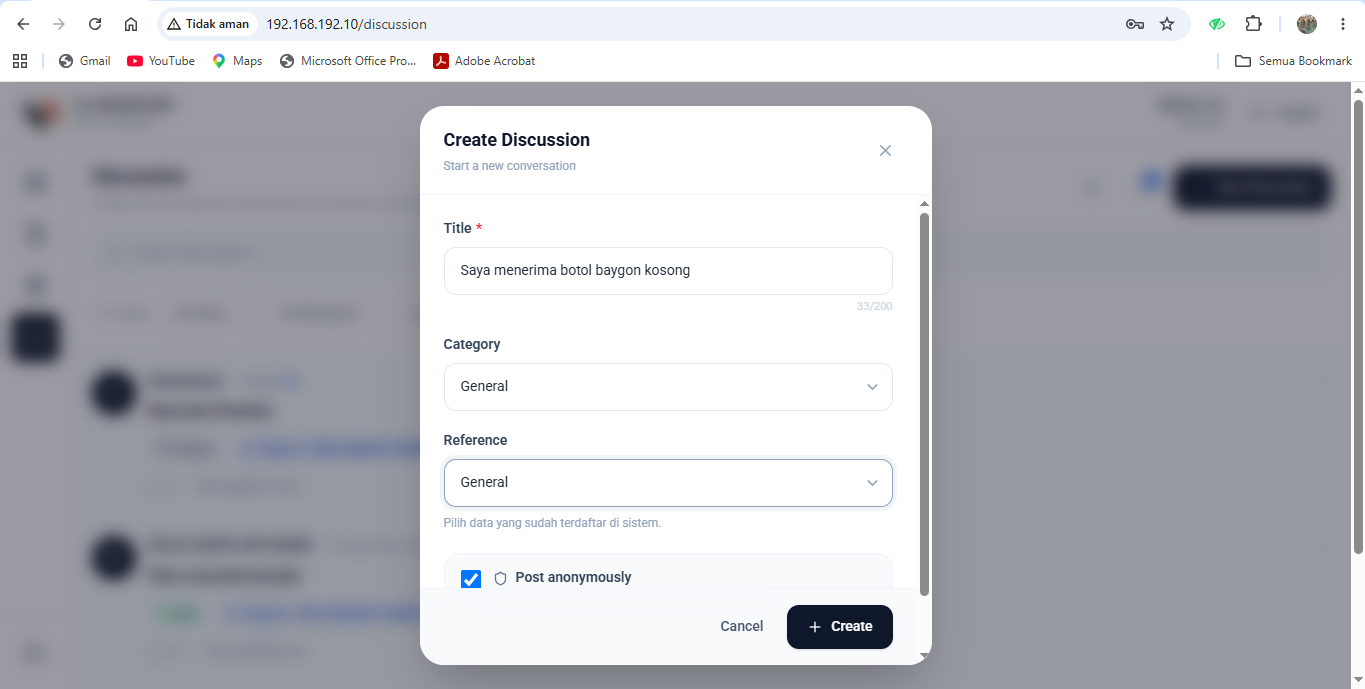
\includegraphics[
						width=0.95\linewidth,
						keepaspectratio
						]{images/Discussion/Discussion3.png}
					}
					
					\only<4>{
						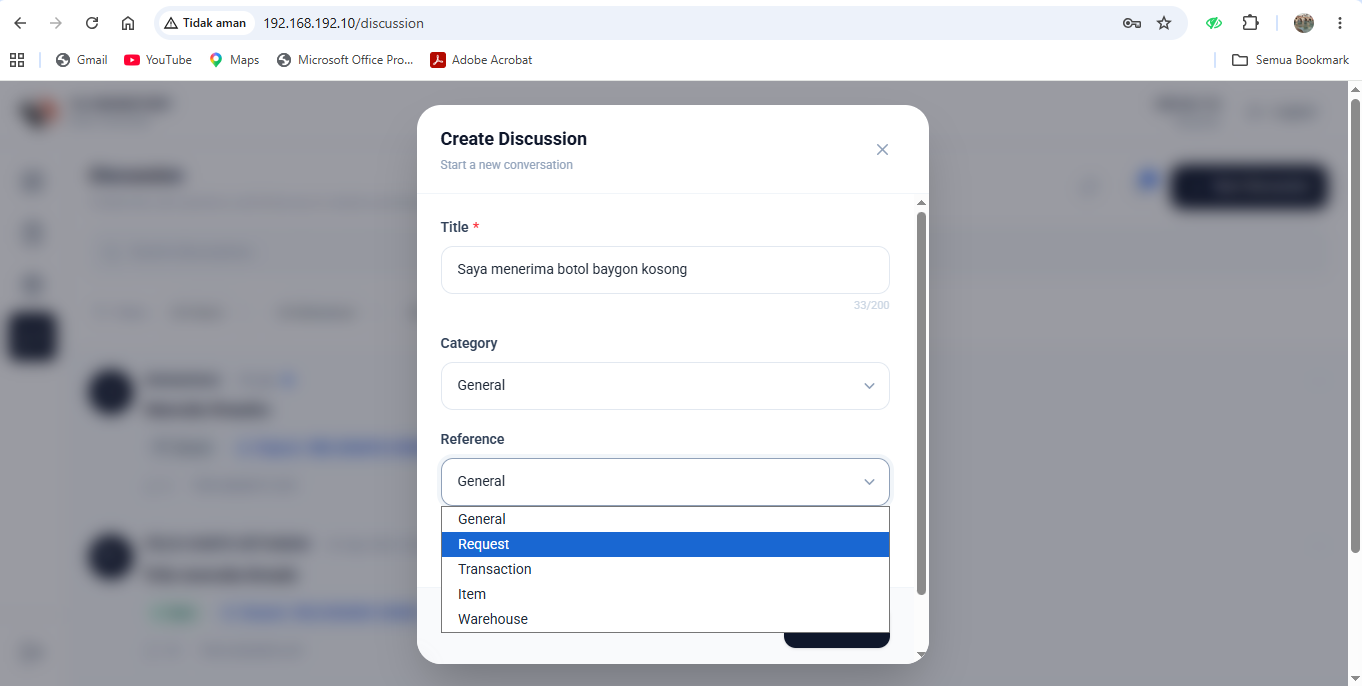
\includegraphics[
						width=0.95\linewidth,
						keepaspectratio
						]{images/Discussion/Discussion4.png}
					}
					
					\only<5>{
						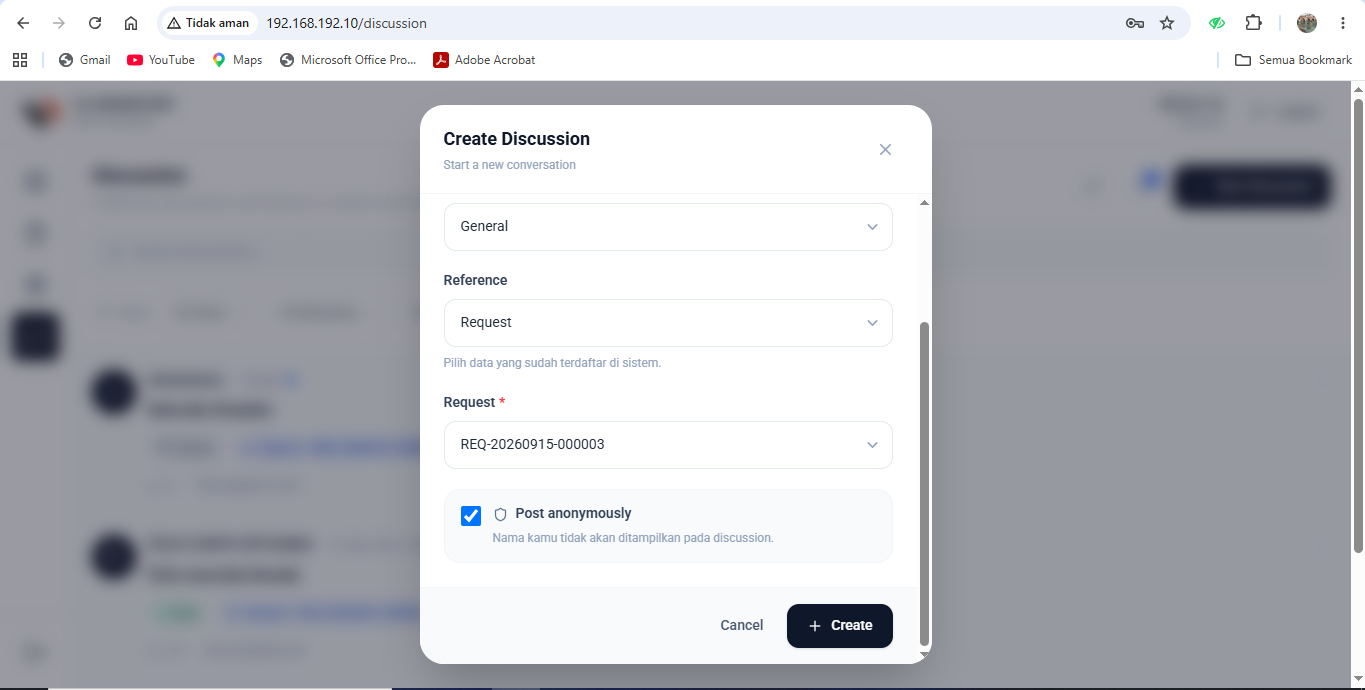
\includegraphics[
						width=0.95\linewidth,
						keepaspectratio
						]{images/Discussion/Discussion5.png}
					}
					
					\only<6>{
						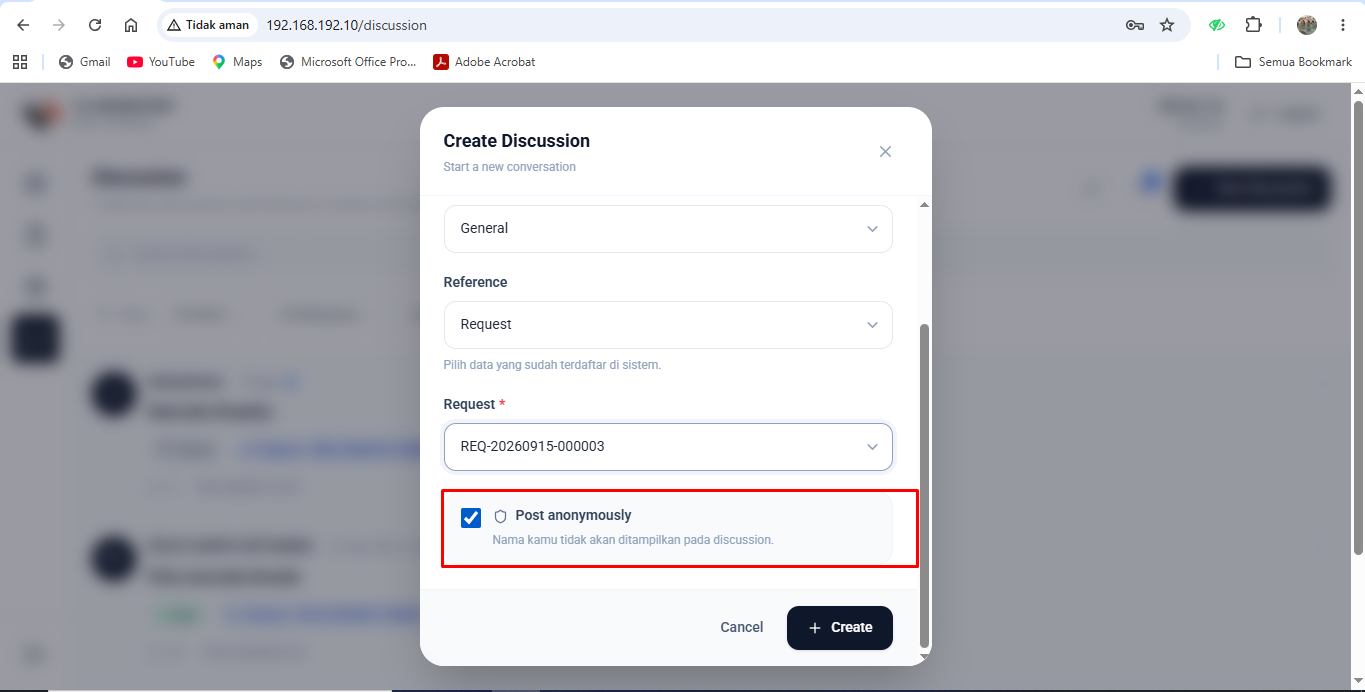
\includegraphics[
						width=0.95\linewidth,
						keepaspectratio
						]{images/Discussion/Discussion6.png}
					}
				};
				
			\end{tikzpicture}
			
		\end{center}
		
		\column{0.025\textwidth}
		
		\column{0.325\textwidth}
		
		\stepcounterdisplay{1}{6}
		\stepcounterdisplay{2}{6}
		\stepcounterdisplay{3}{6}
		\stepcounterdisplay{4}{6}
		\stepcounterdisplay{5}{6}
		\stepcounterdisplay{6}{6}
		
		\sectionlabel{Langkah}
		
		\vspace{0.08cm}
		
		\stepitem{1}{1}{
			Pilih menu \textbf{Discussion}.
		}
		
		\vspace{\TutorialGap}
		
		\stepitem{2}{2}{
			Pilih \textbf{+ New Discussion}.
		}
		
		\vspace{\TutorialGap}
		
		\stepitem{3}{3}{
			Tuliskan keluhan anda di kolom (Title \textcolor{red}{*}).
		}
		
		\vspace{\TutorialGap}
		
		\stepitem{4}{4}{
			Reference digunakan untuk menentukan objek yang menjadi acuan dalam Discussion.\\
				General — untuk pembahasan umum.\\
				Request — untuk pembahasan terkait Request barang.\\
				Transaction — untuk pembahasan terkait transaksi barang.\\
				Item — untuk pembahasan terkait item atau barang tertentu.\\
				Warehouse - untuk pembahasan terkait gudang.\\
		}
		
		\vspace{\TutorialGap}
		
		\stepitem{5}{5}{
			Lampirkan \textbf{Nomor Request/Transaksi} atau \textbf{Nama Item/Gudang} sebagai tagar agar pembahasan lebih mudah dipahami dan ditelusuri.
		}
		
		\vspace{\TutorialGap}
		
		\stepitem{6}{6}{
			Aktifkan \textbf{Post Anonymously} jika Anda ingin
			mengirim Discussion tanpa menampilkan nama Anda. Namun jika tidak diperlukan matikan fitur ini.
		}
		
	\end{columns}
	
\end{frame}
\begin{frame}{07 --- Discussion}
	
	\vspace{-0.25cm}
	
	\begin{columns}[T,totalwidth=\textwidth]
		
		\column{0.65\textwidth}
		
		\begin{center}
			
			\begin{tikzpicture}
				
				\node[
				inner sep=0,
				outer sep=0
				] (screen)
				{
					\only<1>{
						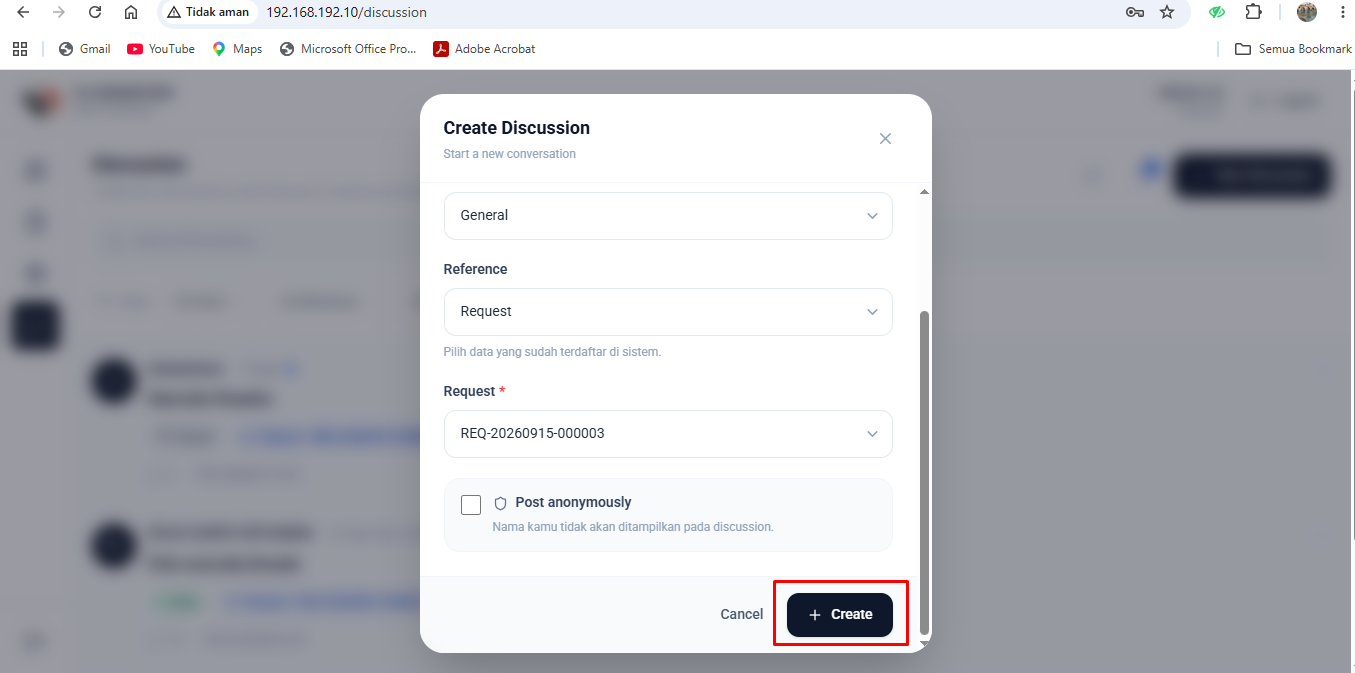
\includegraphics[
						width=0.95\linewidth,
						keepaspectratio
						]{images/Discussion/Discussion7.png}
					}
					
					\only<2>{
						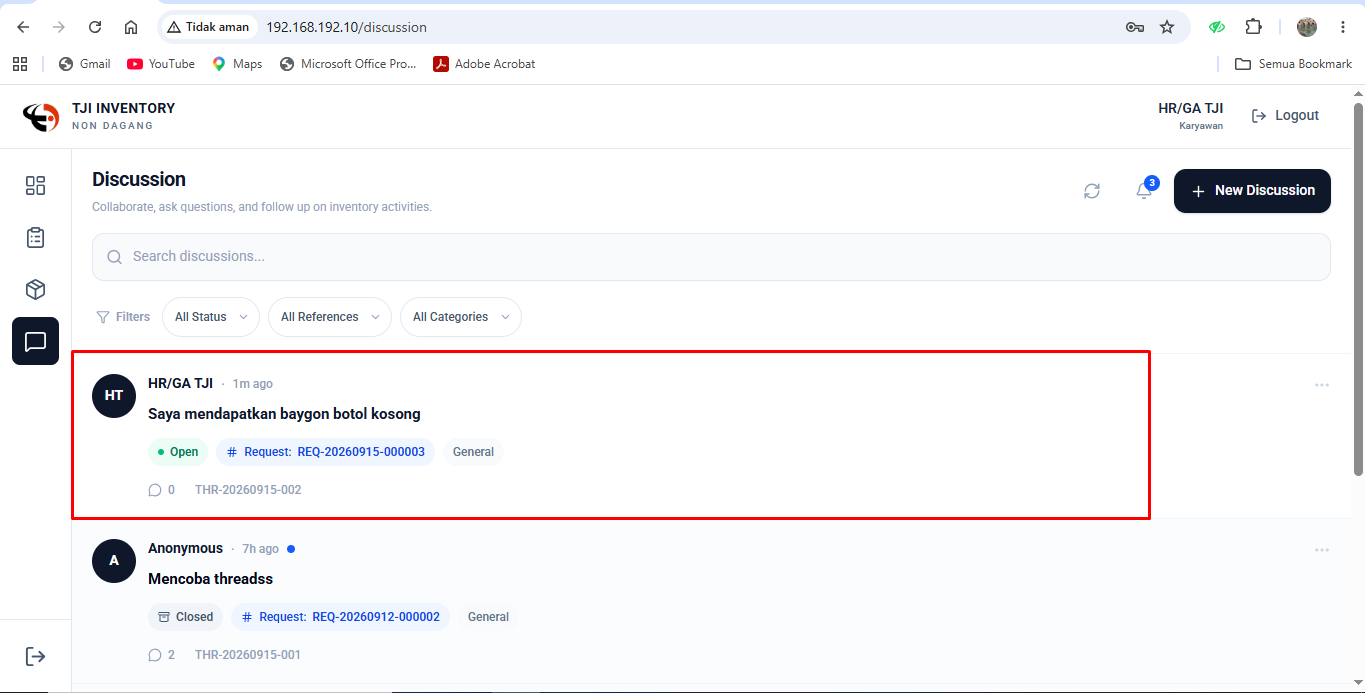
\includegraphics[
						width=0.95\linewidth,
						keepaspectratio
						]{images/Discussion/Discussion8.png}
					}
					
					\only<3>{
						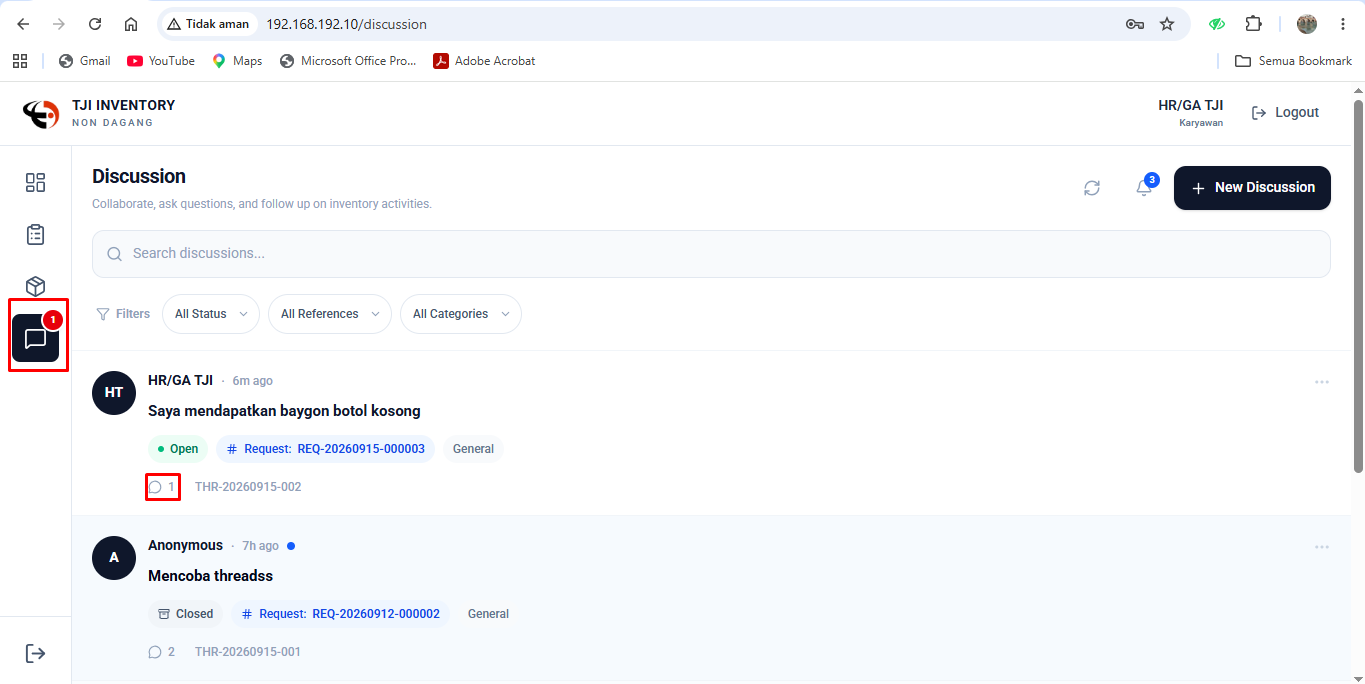
\includegraphics[
						width=0.95\linewidth,
						keepaspectratio
						]{images/Discussion/Discussion9.png}
					}
					
					\only<4>{
						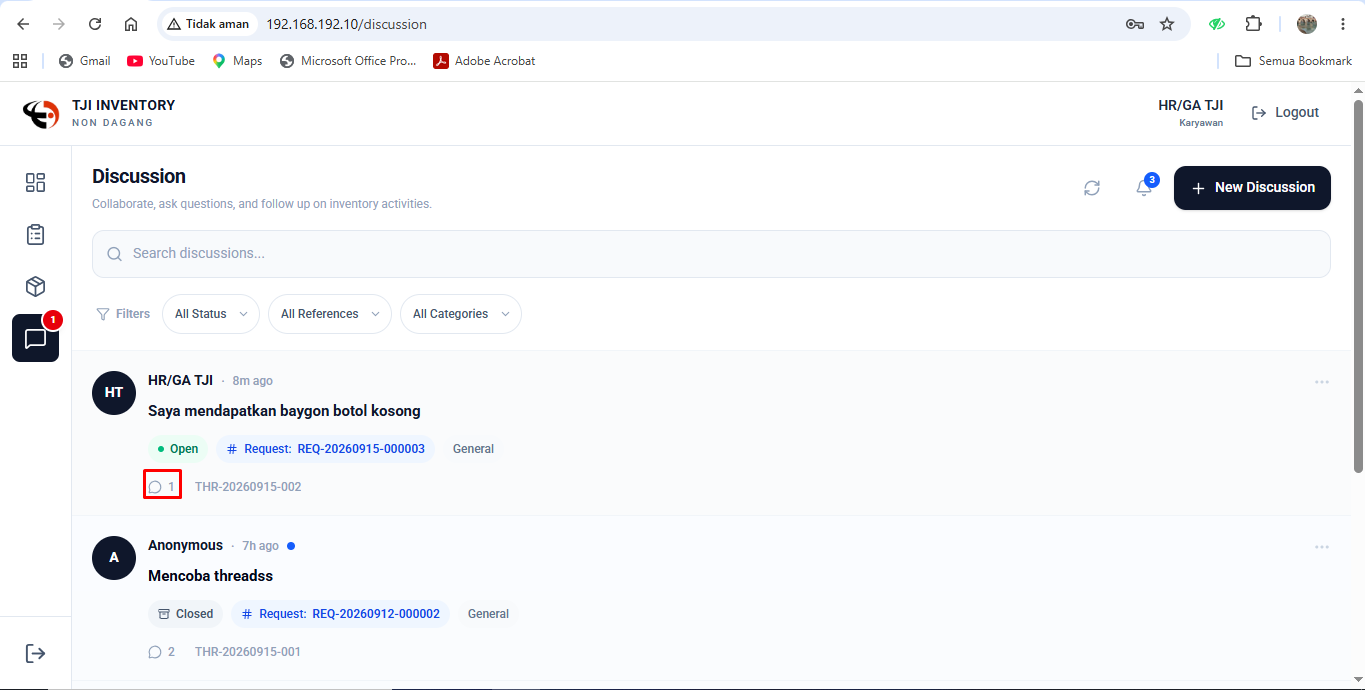
\includegraphics[
						width=0.95\linewidth,
						keepaspectratio
						]{images/Discussion/Discussion10.png}
					}
					
					\only<5>{
						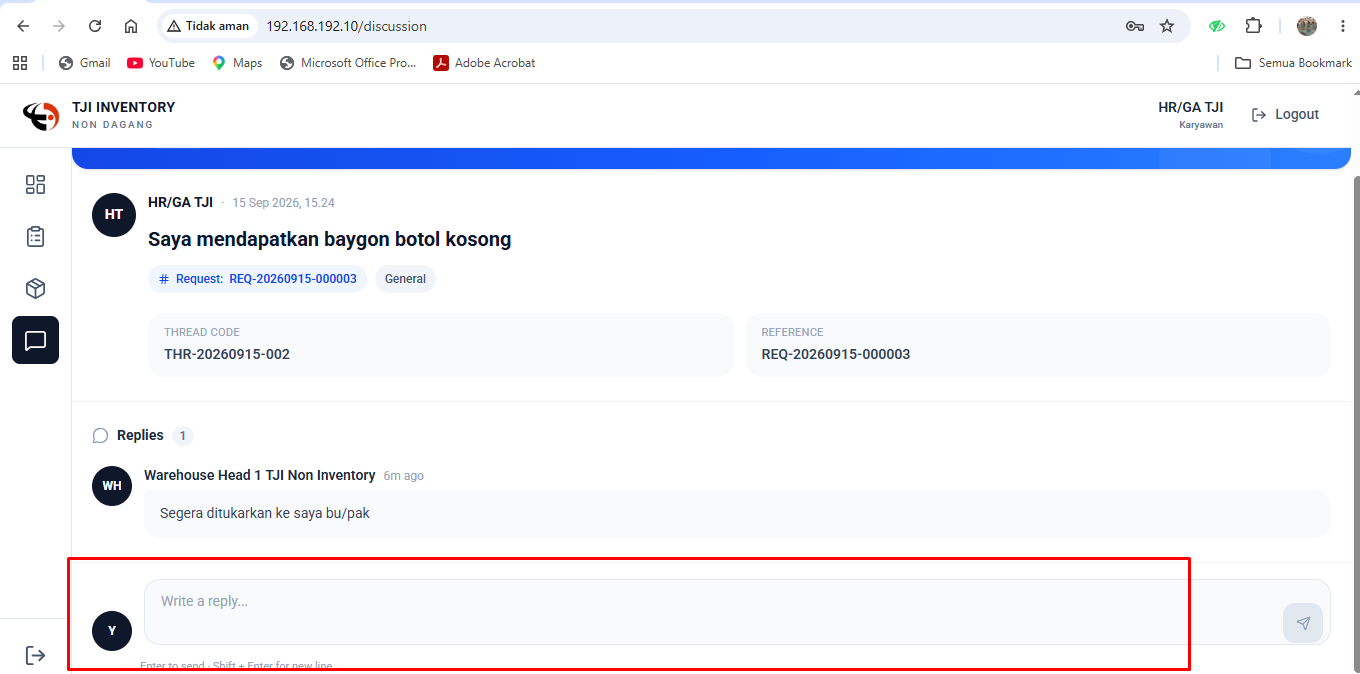
\includegraphics[
						width=0.95\linewidth,
						keepaspectratio
						]{images/Discussion/Discussion11.png}
					}
					
					\only<6>{
						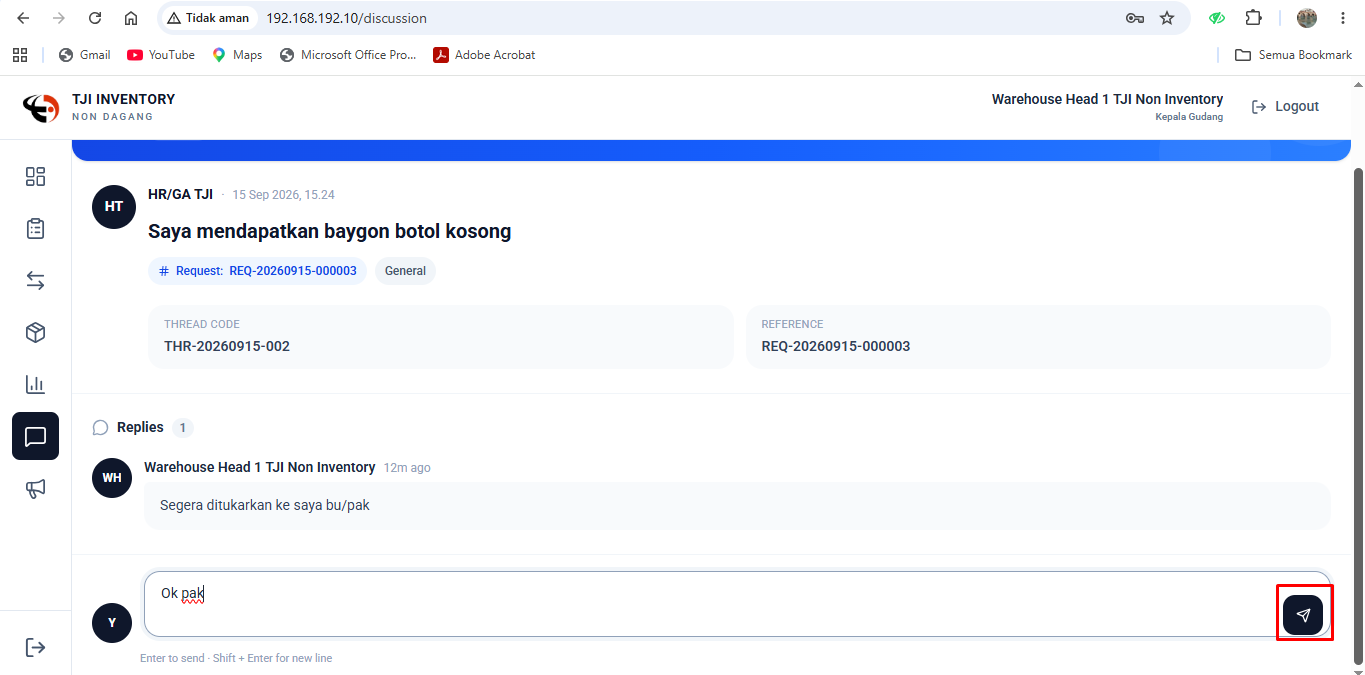
\includegraphics[
						width=0.95\linewidth,
						keepaspectratio
						]{images/Discussion/Discussion12.png}
					}
					
					\only<7>{
						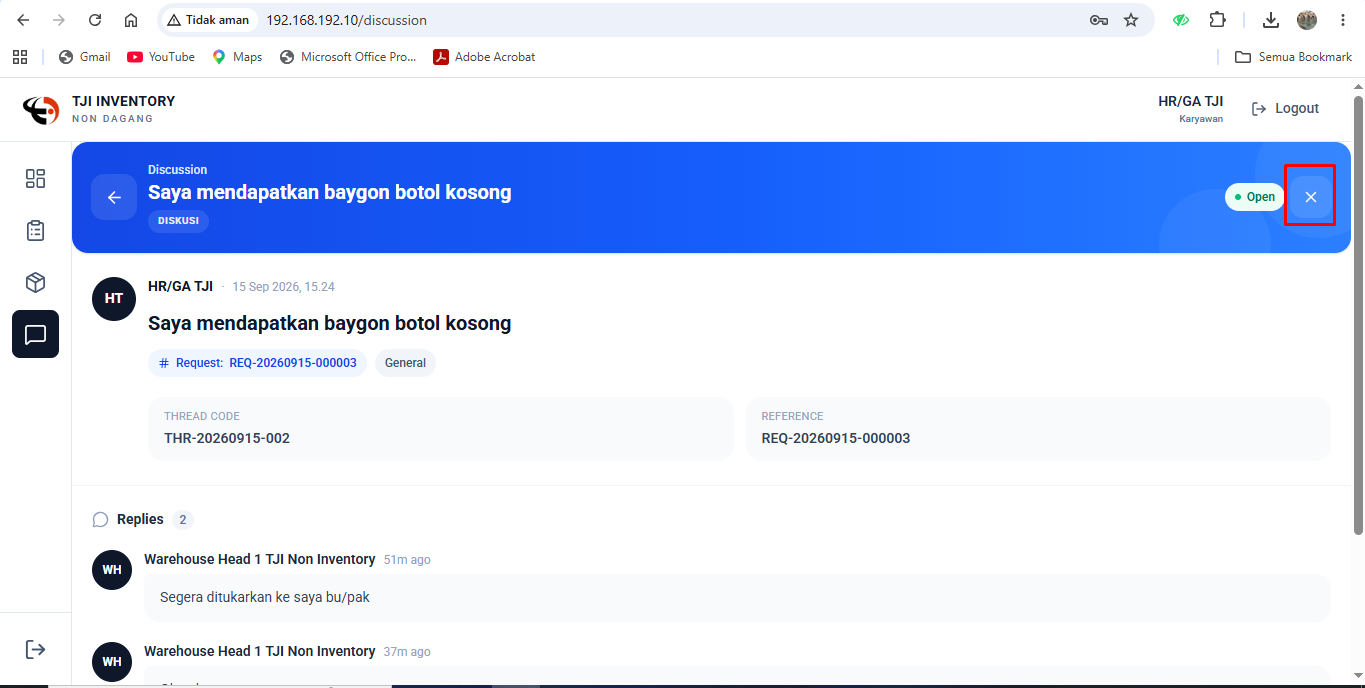
\includegraphics[
						width=0.95\linewidth,
						keepaspectratio
						]{images/Discussion/Discussion13.png}
					}
				};
				
			\end{tikzpicture}
			
		\end{center}
		
		\column{0.025\textwidth}
		
		\column{0.325\textwidth}
		
		\stepcounterdisplay{1}{7}
		\stepcounterdisplay{2}{7}
		\stepcounterdisplay{3}{7}
		\stepcounterdisplay{4}{7}
		\stepcounterdisplay{5}{7}
		\stepcounterdisplay{6}{7}
		\stepcounterdisplay{7}{7}
		
		\sectionlabel{Langkah}
		
		\vspace{0.08cm}
		
		\stepitem{1}{1}{
			Pilih \textbf{+ Create} untuk
			membuat Discussion.
		}
		
		\vspace{\TutorialGap}
		
		\stepitem{2}{2}{
			Pastikan Discussion berhasil dibuat
			dan tampil pada daftar Discussion.
		}
		
		\vspace{\TutorialGap}
		
		\stepitem{3}{3}{
			Jika terdapat balasan pada Discussion,
			akan muncul indikator berwarna merah.
		}
		
		\vspace{\TutorialGap}
		
		\stepitem{4}{4}{
			Pilih ikon dialog untuk melihat
			pesan atau tanggapan.
		}
		
		\vspace{\TutorialGap}
		
		\stepitem{5}{5}{
			Baca pesan tanggapan, kemudian
			tuliskan balasan pada kolom yang tersedia.
		}
		
		\vspace{\TutorialGap}
		
		\stepitem{6}{6}{
			Pilih ikon \textbf{Pesawat} untuk
			mengirim balasan.
		}
		
		\vspace{\TutorialGap}
		
		\stepitem{7}{7}{
			Jika pembahasan sudah selesai, pilih ikon \textbf{(X)} untuk menutup ruang Discussion.
		}
		
	\end{columns}
	
\end{frame}

% =========================================================
% CLOSING
% =========================================================


{
	\setbeamertemplate{footline}{}
	
	\begin{frame}
		
		\centering
		
		\vspace{1.15cm}
		
		{\fontsize{38}{44}\selectfont
			\textbf{\color{Primary}THANK YOU}
		}
		
		\vspace{0.55cm}
		
		{\fontsize{22}{27}\selectfont
			TJI Inventory Non Dagang
		}
		
		\vspace{0.85cm}
		
		\begin{center}
			
			\begin{tikzpicture}
				
				\node[
				draw=Primary,
				line width=1pt,
				fill=Secondary,
				rounded corners=6pt,
				inner xsep=18pt,
				inner ysep=12pt,
				text width=0.65\textwidth,
				align=center
				]{
					
					{\fontsize{18}{22}\selectfont
						\textbf{\color{Primary}Terima Kasih Atas Perhatian Anda}}
					
					\\[5pt]
					
					{\fontsize{15.5}{20}\selectfont
						Hubungi administrator aplikasi apabila mengalami
						kendala dalam penggunaan sistem.
					}
					
				};
				
			\end{tikzpicture}
			
		\end{center}
		
		\vfill
		
		{\fontsize{14}{18}\selectfont
			PT Timur Jaya Indo Steel -- 2026
		}
		
		\vspace{0.45cm}
		
	\end{frame}
	
}



\end{document}

